Figs.\ref{fig:hijing_data_mc_particle_ratios}, \ref{fig:epos_data_mc_particle_ratios} and \ref{fig:ampt_data_mc_particle_ratios} show the data to MC ratios used as particle reweighting factors for the three MC generators used in the \detdeta analysis: \hijing, \epos and \ampt.
To construct these ratios truth particle spectra from MC generators was compared to particle spectra from PHENIX and STAR~\cite{phenix_particle_spectra,star_lambda_spectra}.

\begin{figure}
    \centering
    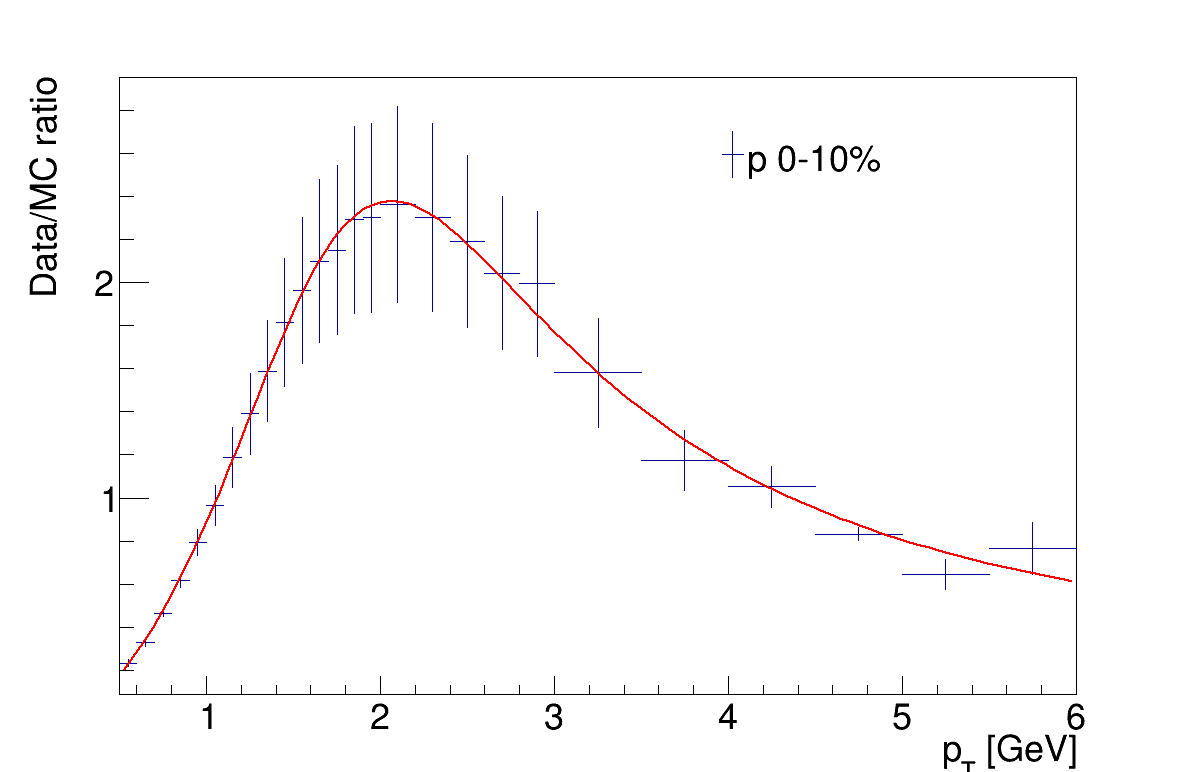
\includegraphics[width=0.24\linewidth]{detdeta/Figures/particle_reweighting_ratios/HIJING_p_0.png}
    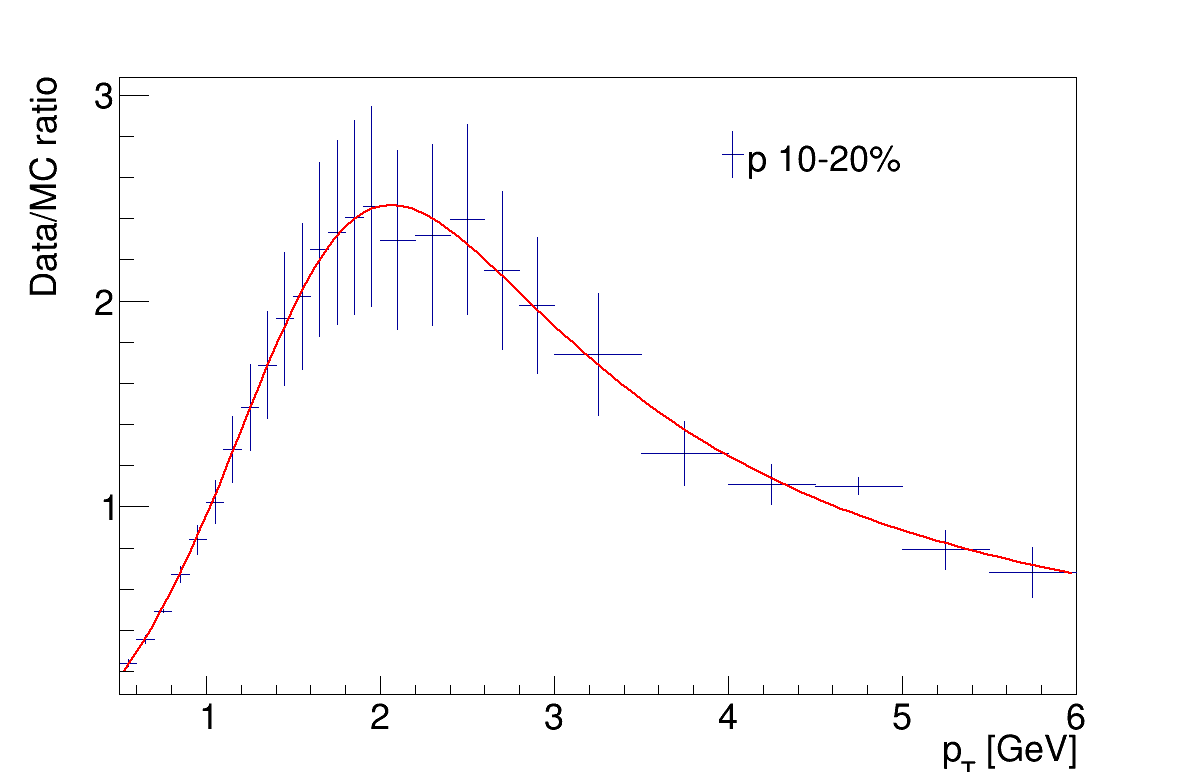
\includegraphics[width=0.24\linewidth]{detdeta/Figures/particle_reweighting_ratios/HIJING_p_1.png}
    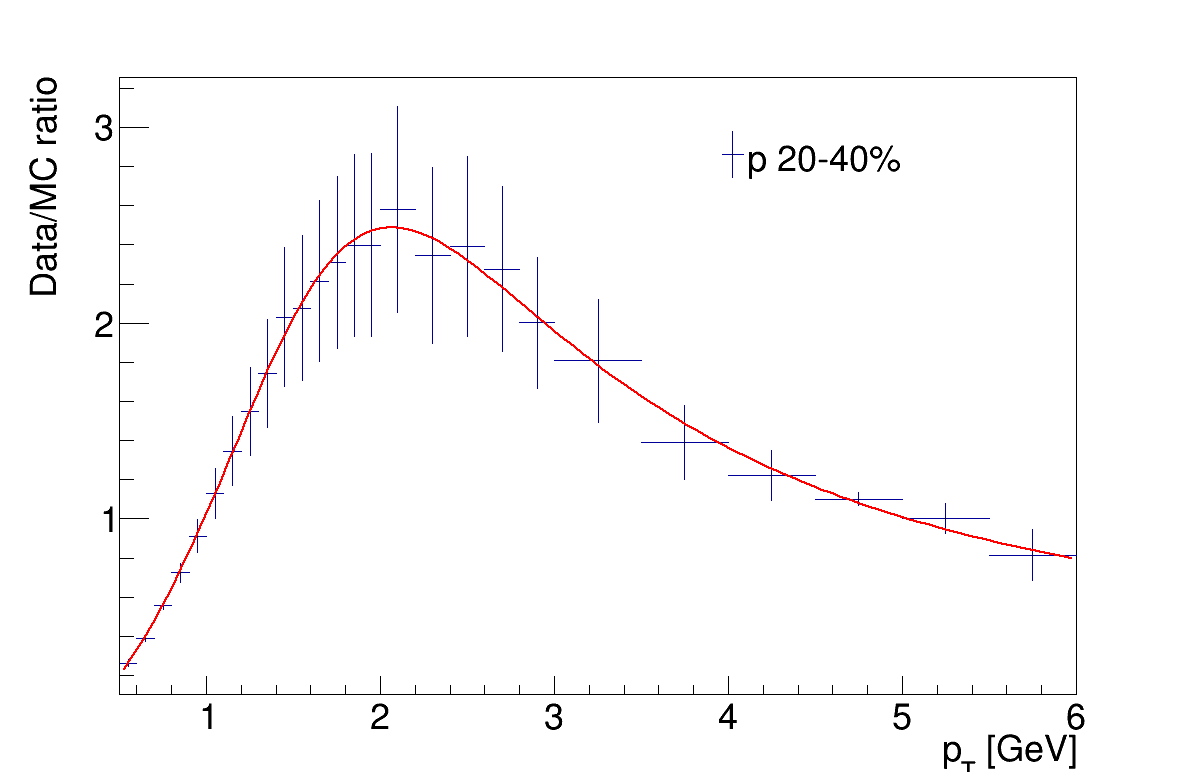
\includegraphics[width=0.24\linewidth]{detdeta/Figures/particle_reweighting_ratios/HIJING_p_2.png}
    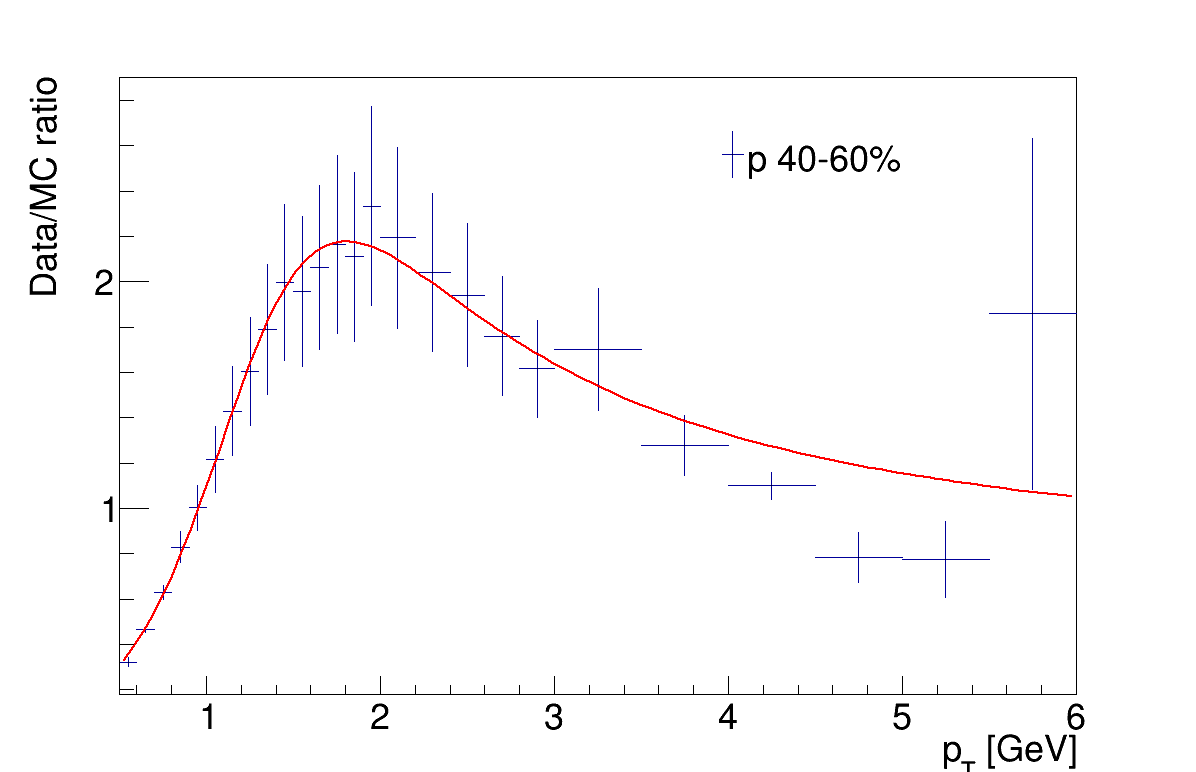
\includegraphics[width=0.24\linewidth]{detdeta/Figures/particle_reweighting_ratios/HIJING_p_3.png}
    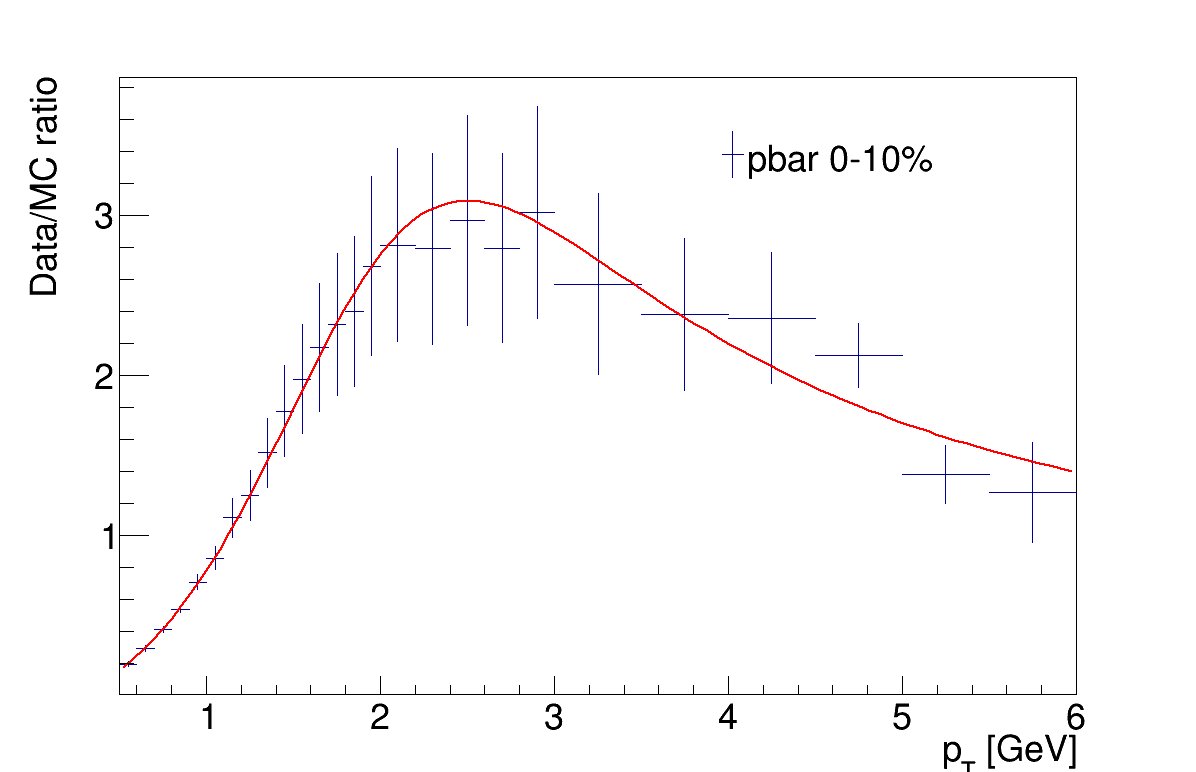
\includegraphics[width=0.24\linewidth]{detdeta/Figures/particle_reweighting_ratios/HIJING_pbar_0.png}
    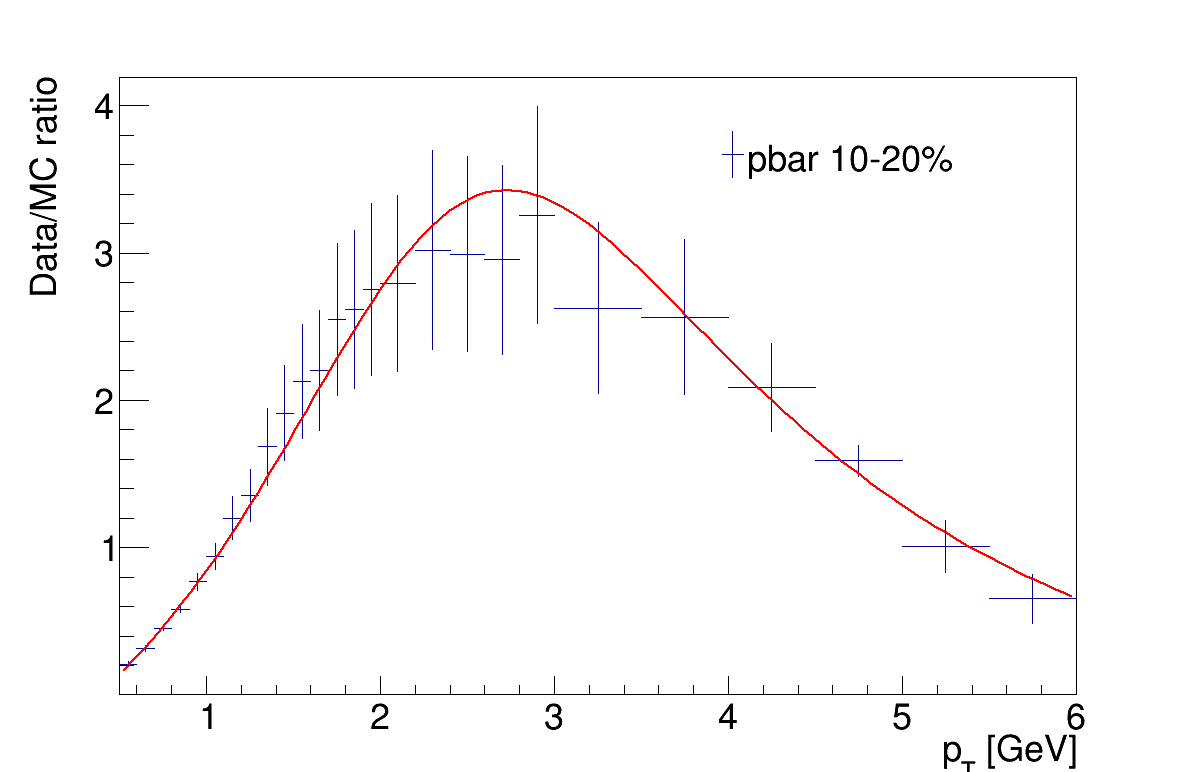
\includegraphics[width=0.24\linewidth]{detdeta/Figures/particle_reweighting_ratios/HIJING_pbar_1.png}
    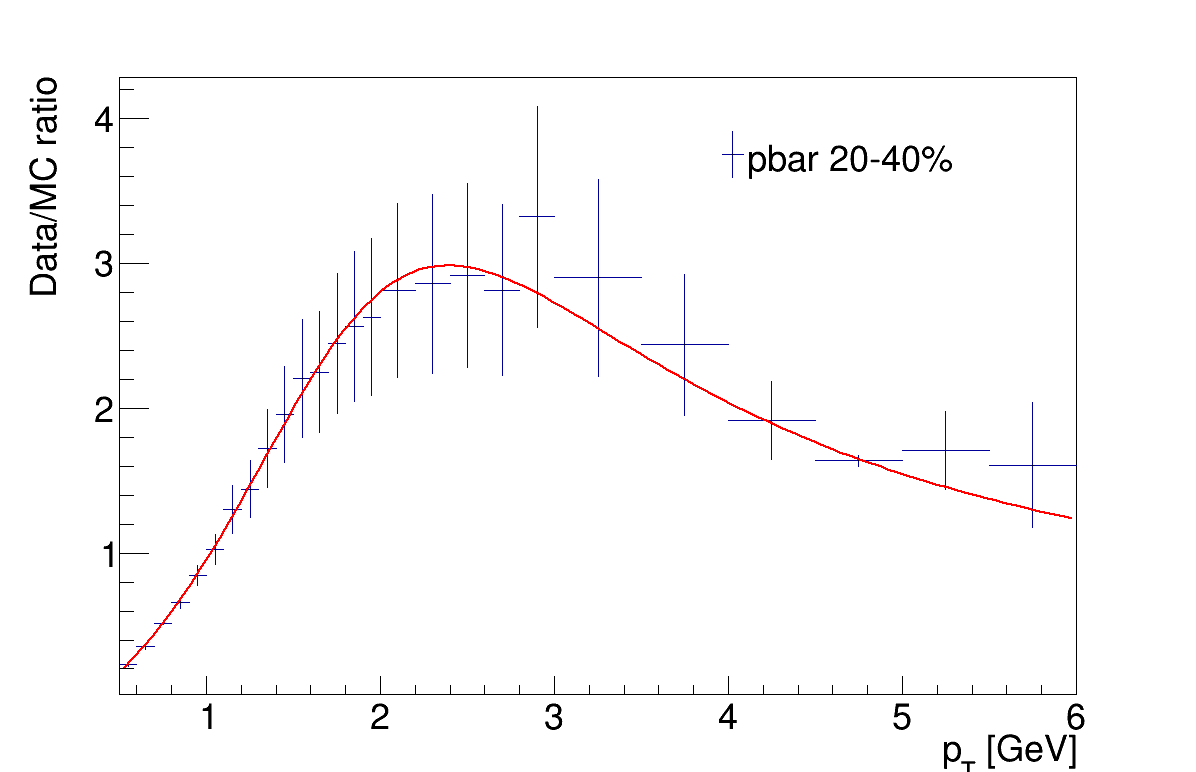
\includegraphics[width=0.24\linewidth]{detdeta/Figures/particle_reweighting_ratios/HIJING_pbar_2.png}
    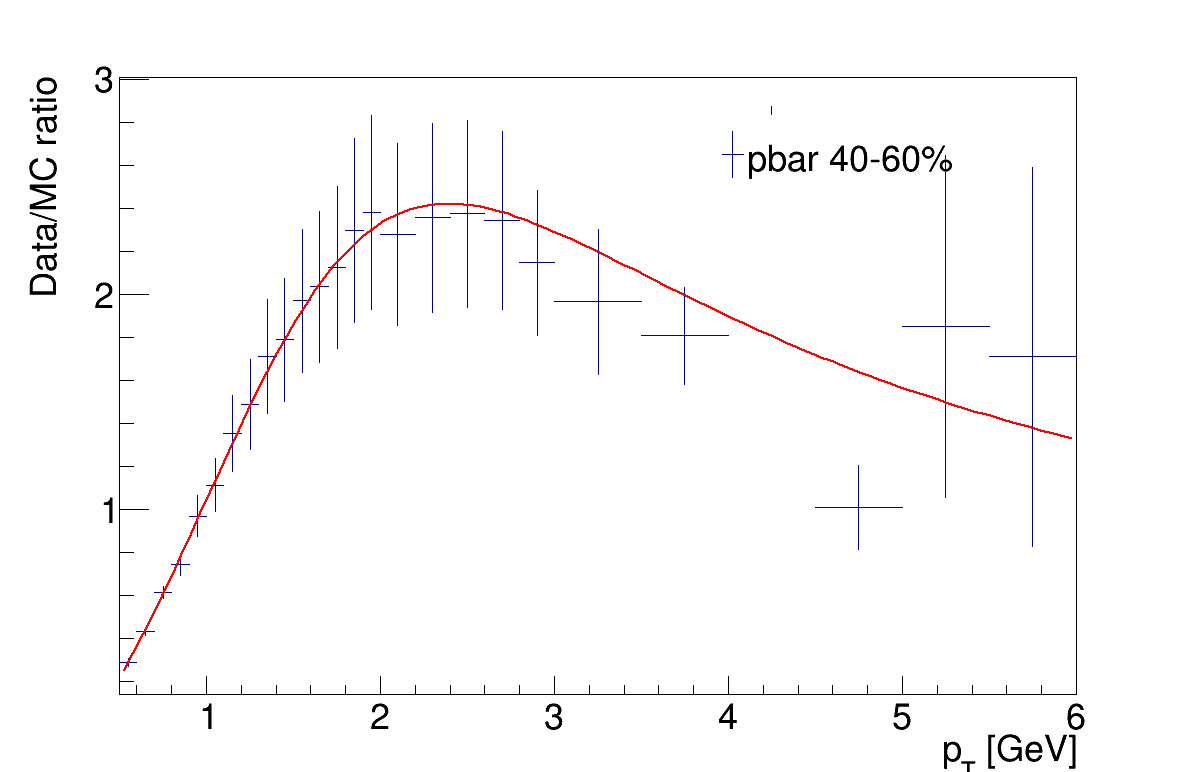
\includegraphics[width=0.24\linewidth]{detdeta/Figures/particle_reweighting_ratios/HIJING_pbar_3.png}
    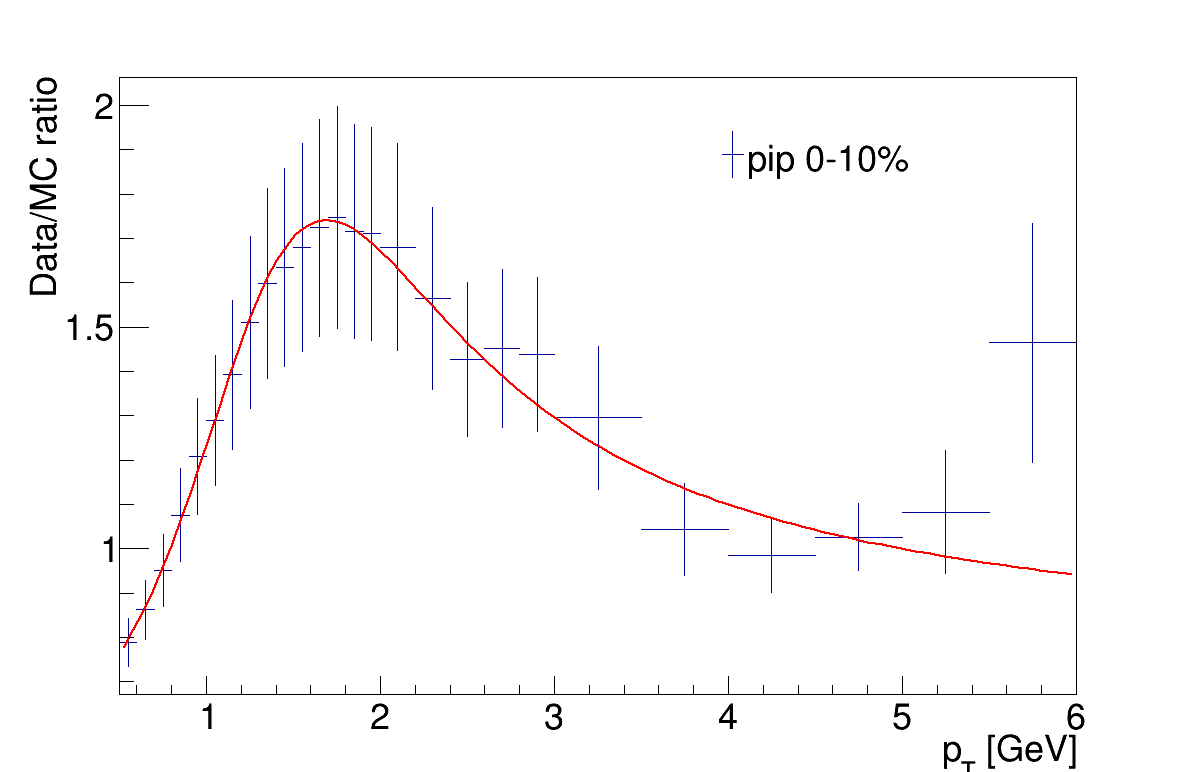
\includegraphics[width=0.24\linewidth]{detdeta/Figures/particle_reweighting_ratios/HIJING_pip_0.png}
    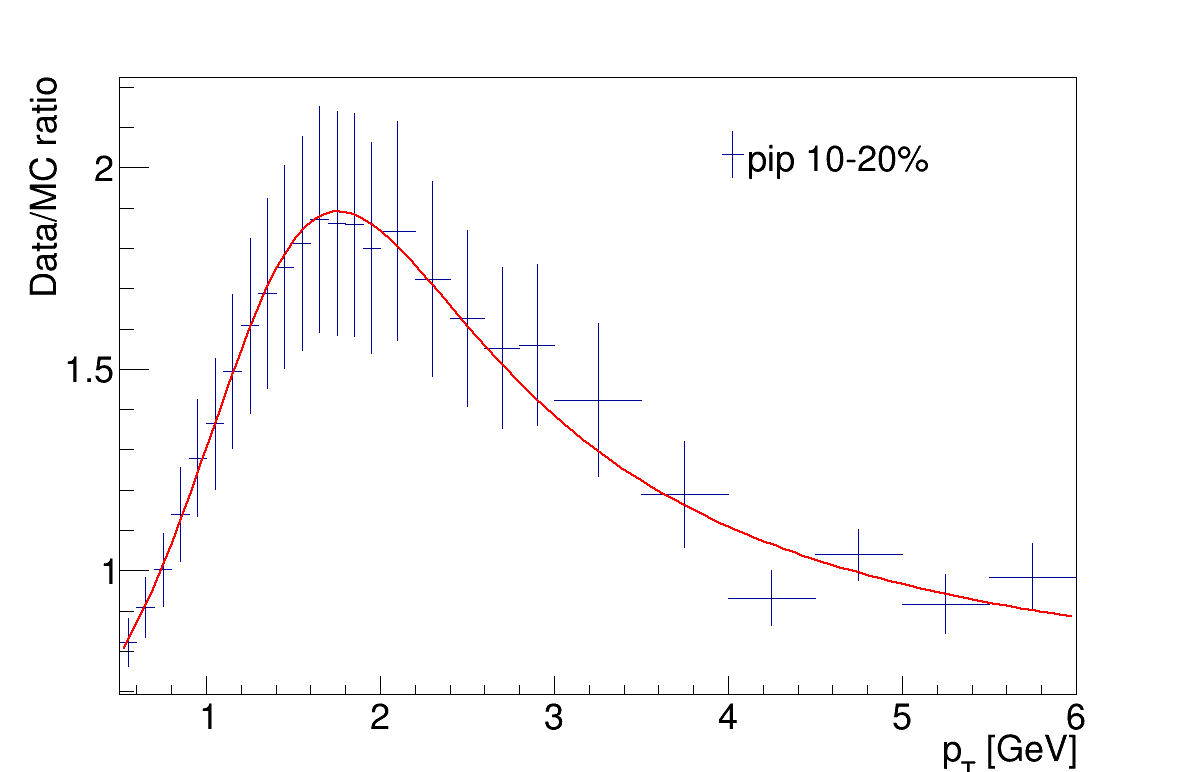
\includegraphics[width=0.24\linewidth]{detdeta/Figures/particle_reweighting_ratios/HIJING_pip_1.png}
    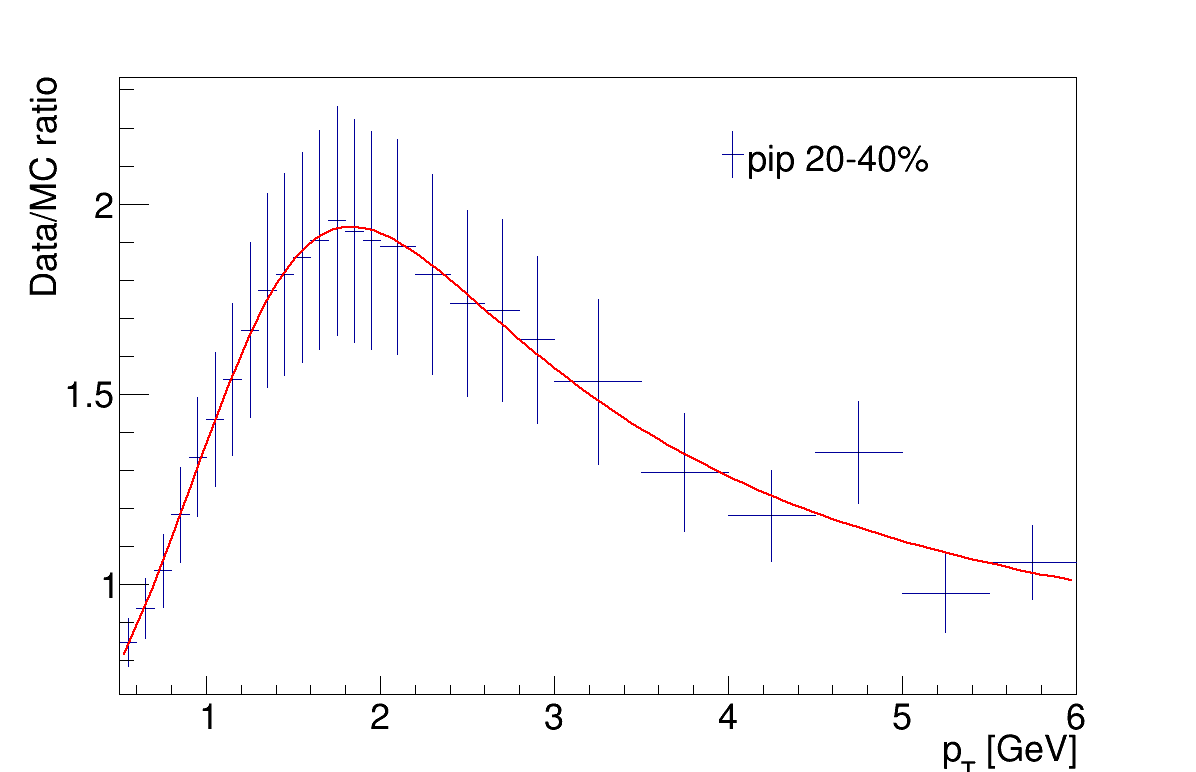
\includegraphics[width=0.24\linewidth]{detdeta/Figures/particle_reweighting_ratios/HIJING_pip_2.png}
    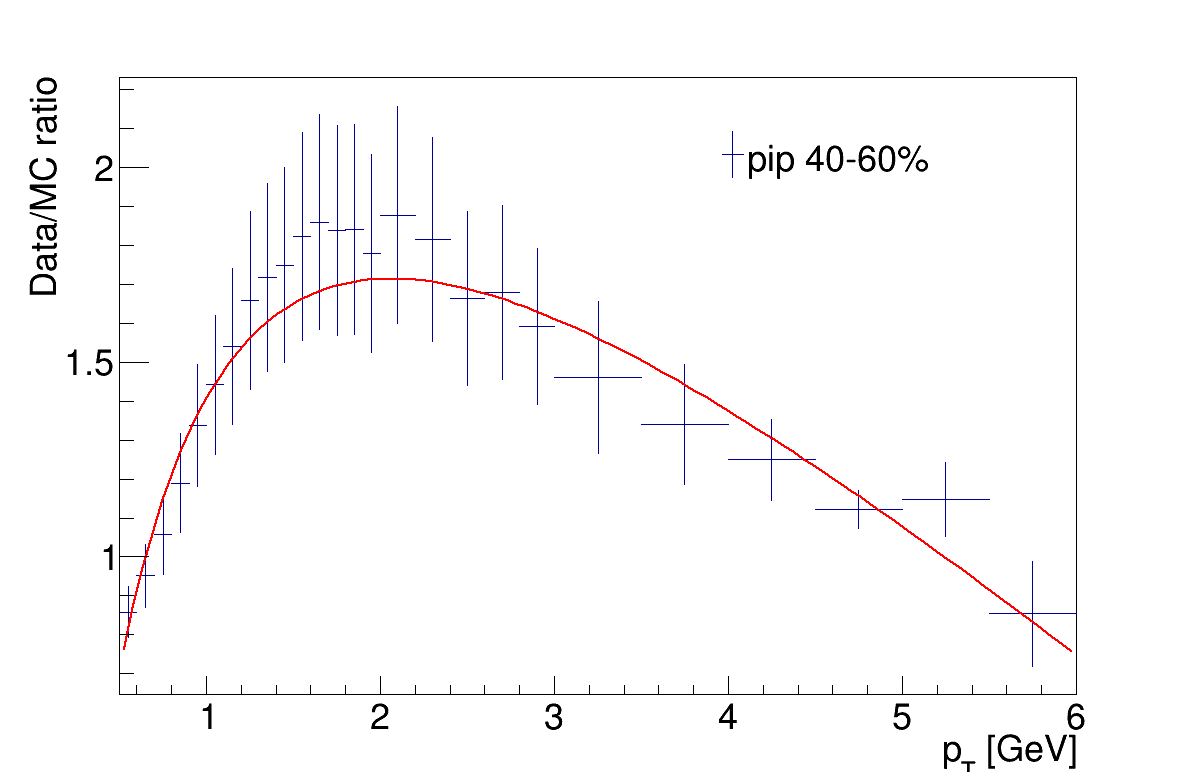
\includegraphics[width=0.24\linewidth]{detdeta/Figures/particle_reweighting_ratios/HIJING_pip_3.png}
    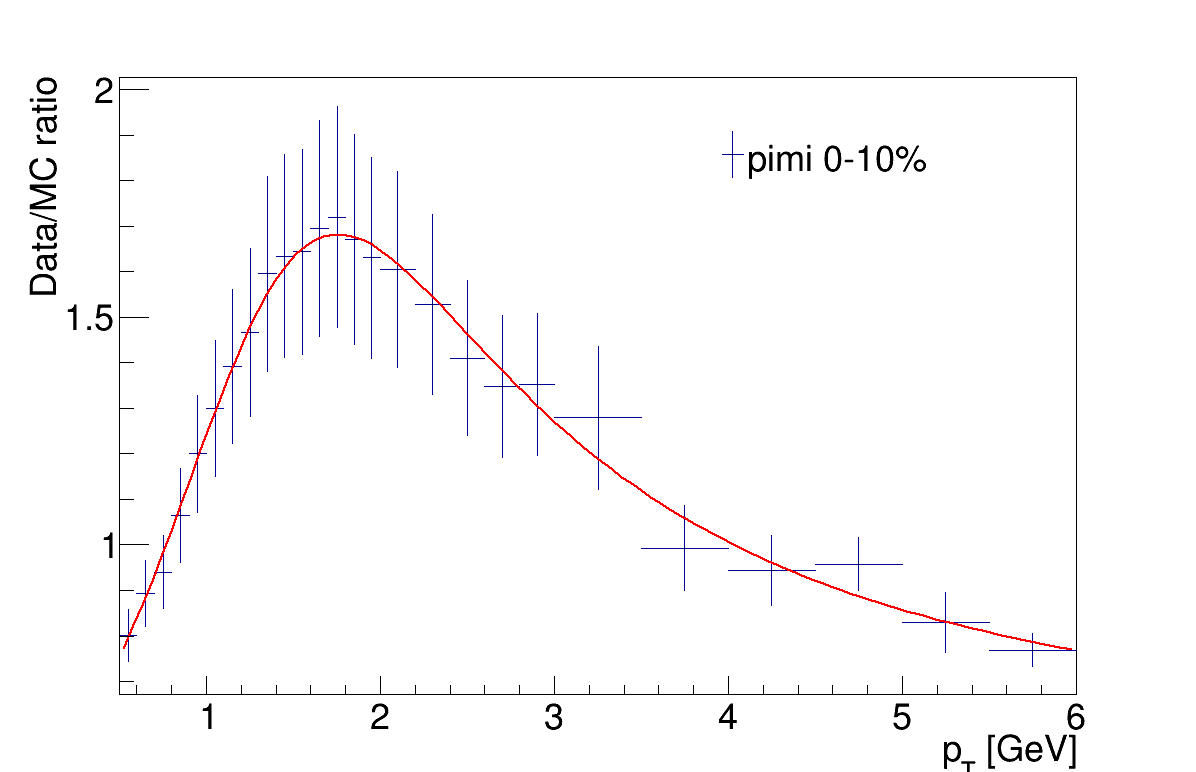
\includegraphics[width=0.24\linewidth]{detdeta/Figures/particle_reweighting_ratios/HIJING_pimi_0.png}
    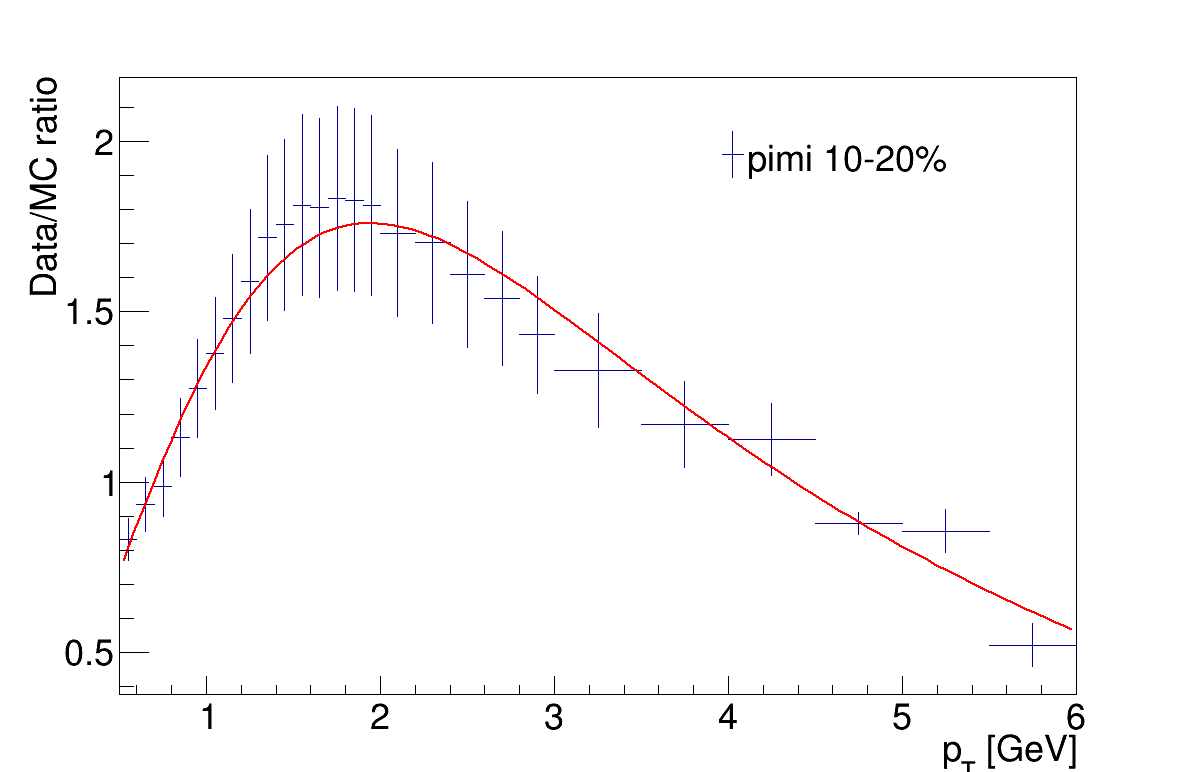
\includegraphics[width=0.24\linewidth]{detdeta/Figures/particle_reweighting_ratios/HIJING_pimi_1.png}
    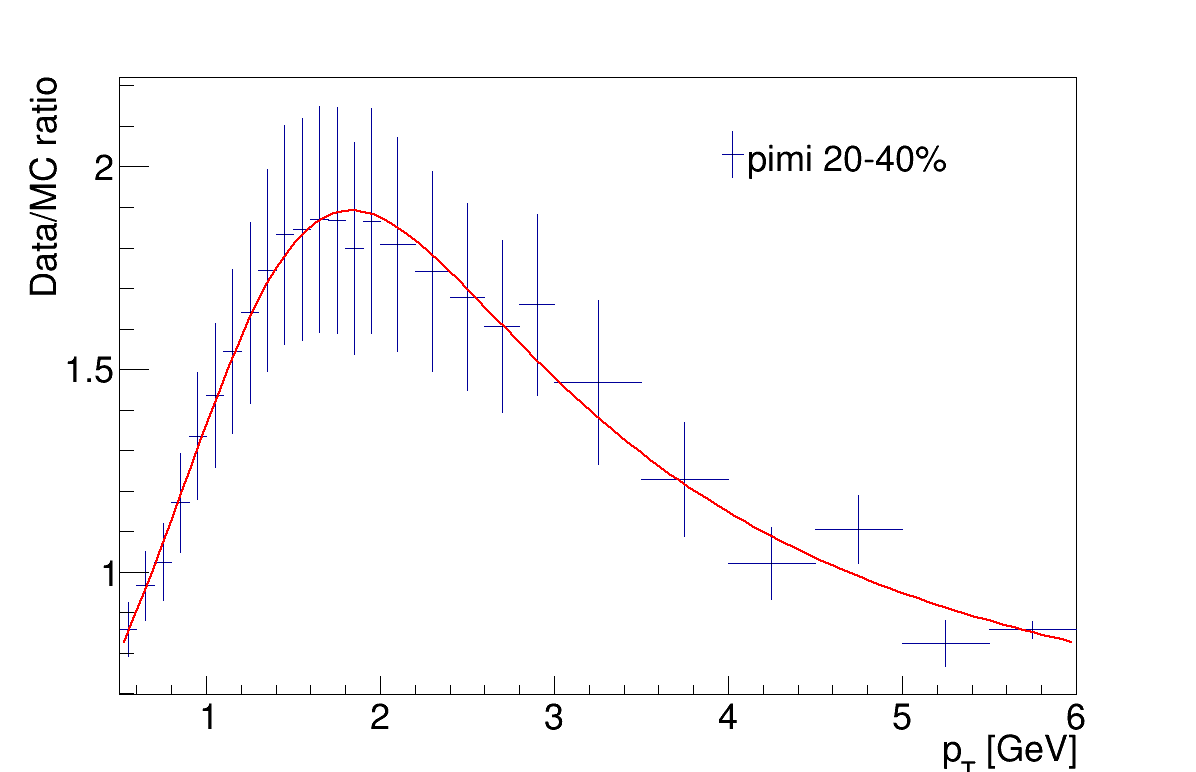
\includegraphics[width=0.24\linewidth]{detdeta/Figures/particle_reweighting_ratios/HIJING_pimi_2.png}
    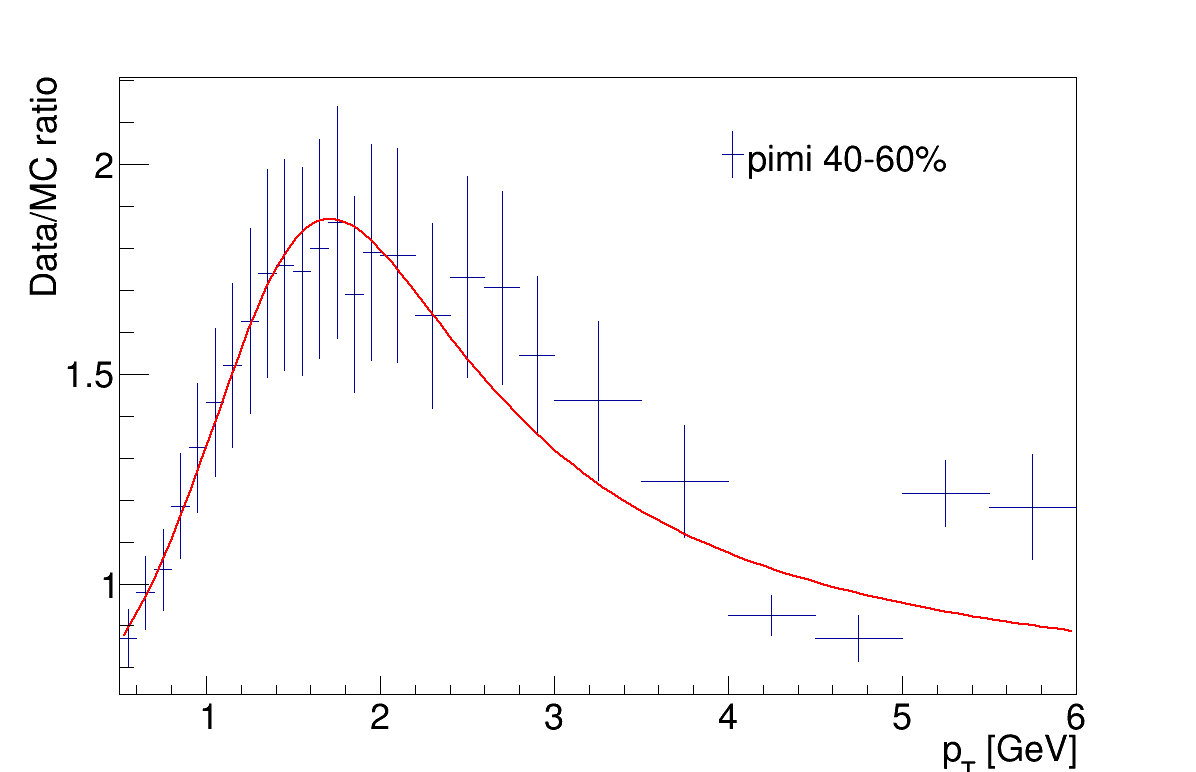
\includegraphics[width=0.24\linewidth]{detdeta/Figures/particle_reweighting_ratios/HIJING_pimi_3.png}
    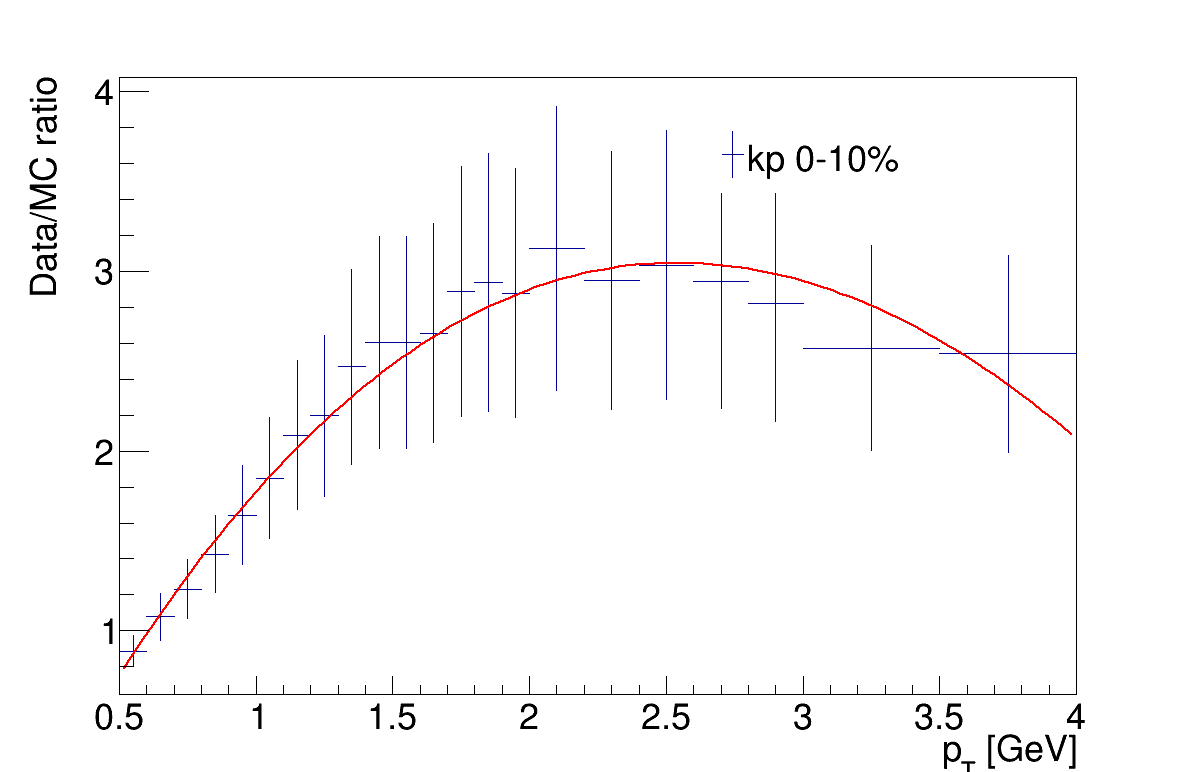
\includegraphics[width=0.24\linewidth]{detdeta/Figures/particle_reweighting_ratios/HIJING_kp_0.png}
    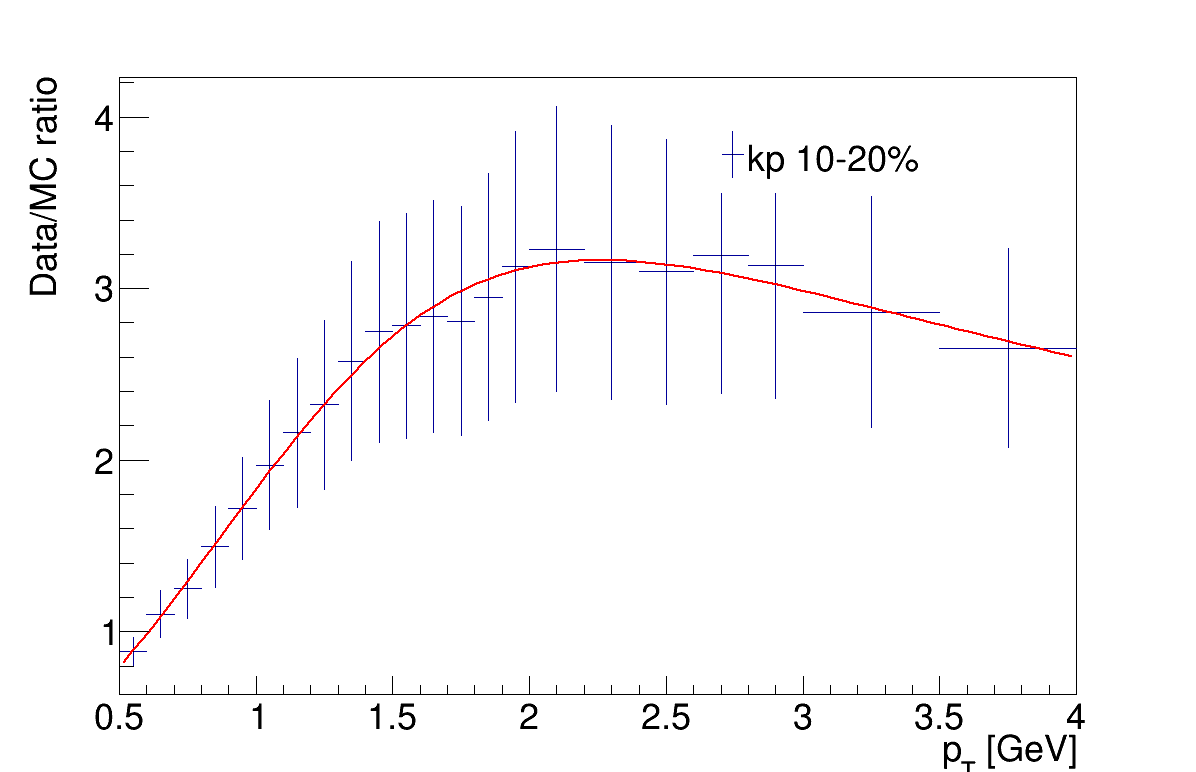
\includegraphics[width=0.24\linewidth]{detdeta/Figures/particle_reweighting_ratios/HIJING_kp_1.png}
    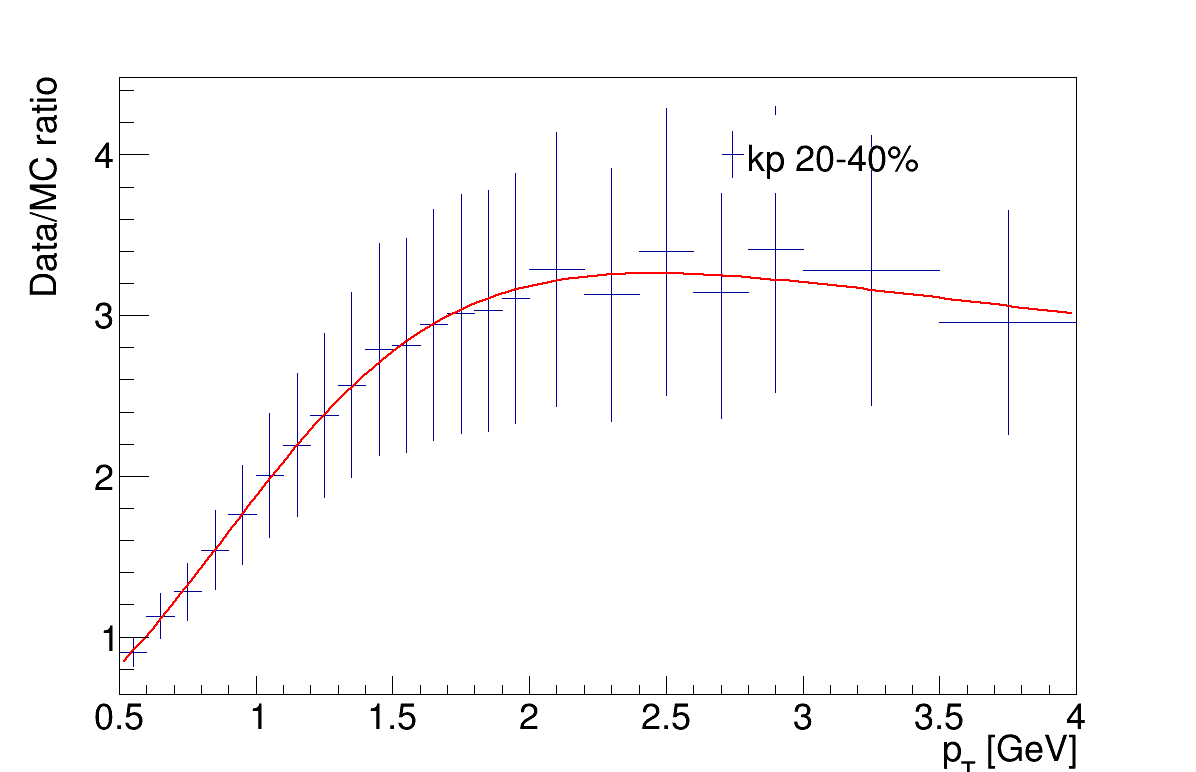
\includegraphics[width=0.24\linewidth]{detdeta/Figures/particle_reweighting_ratios/HIJING_kp_2.png}
    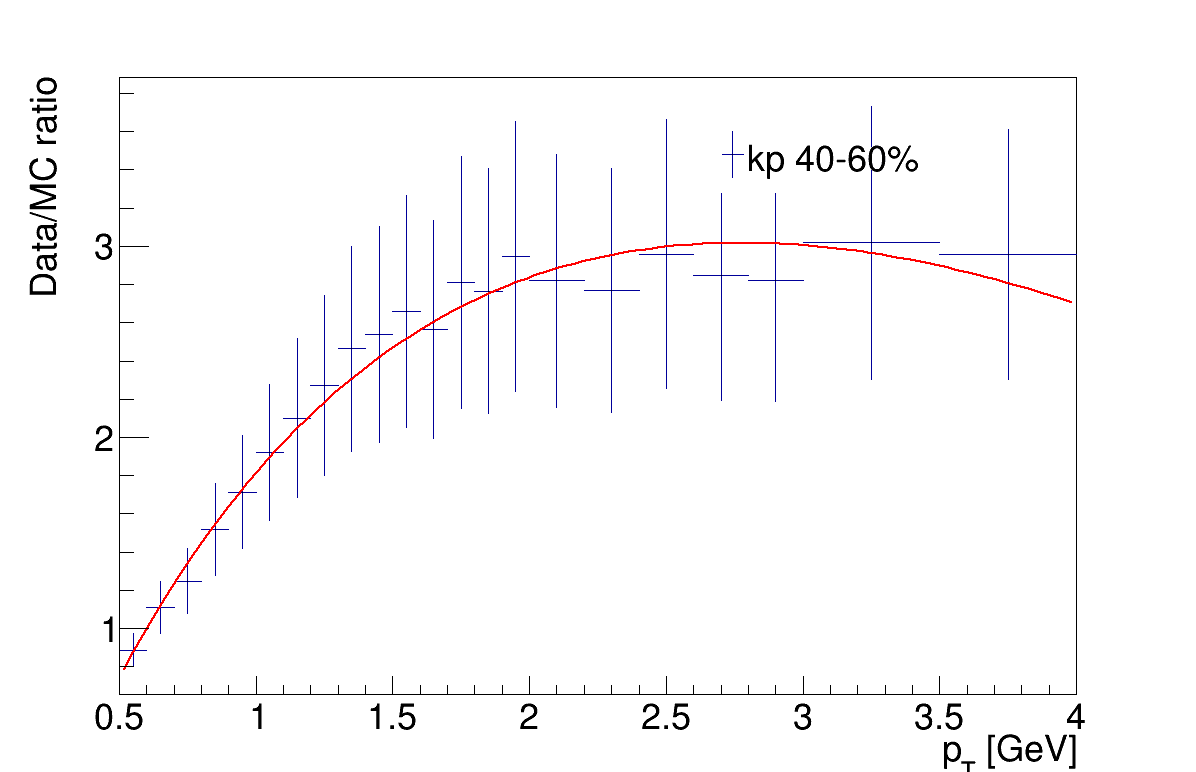
\includegraphics[width=0.24\linewidth]{detdeta/Figures/particle_reweighting_ratios/HIJING_kp_3.png}
    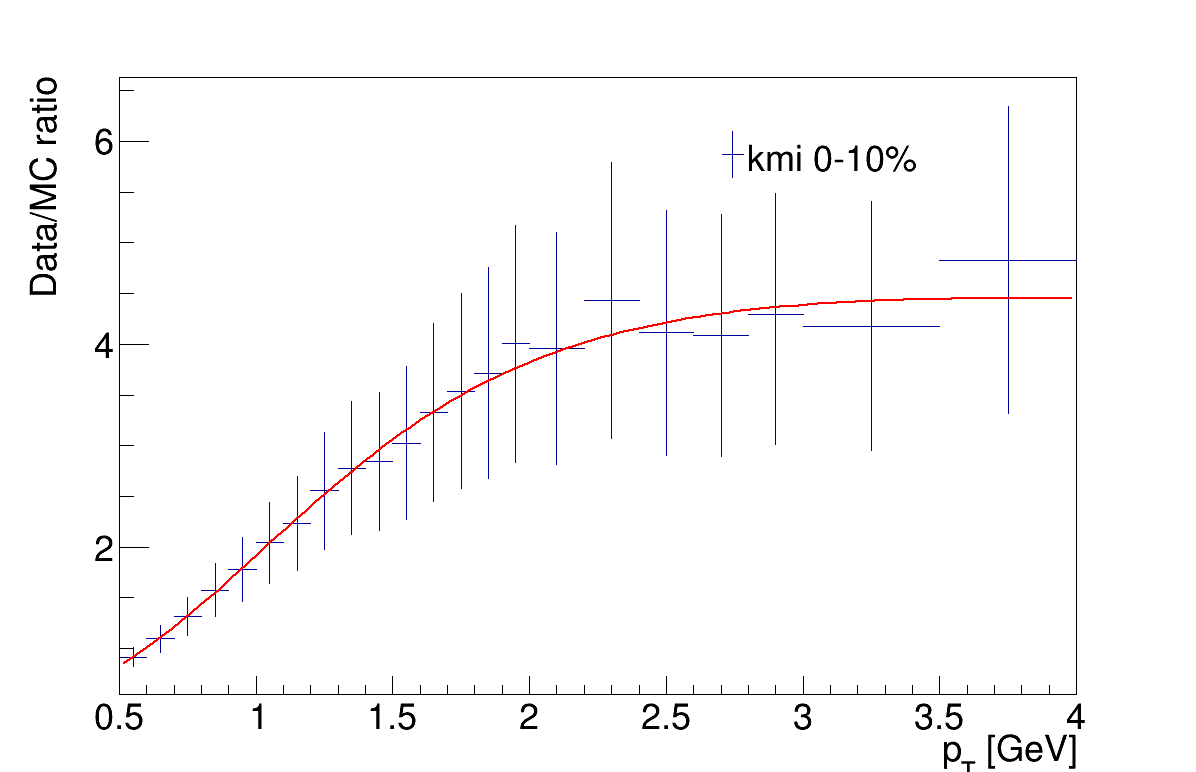
\includegraphics[width=0.24\linewidth]{detdeta/Figures/particle_reweighting_ratios/HIJING_kmi_0.png}
    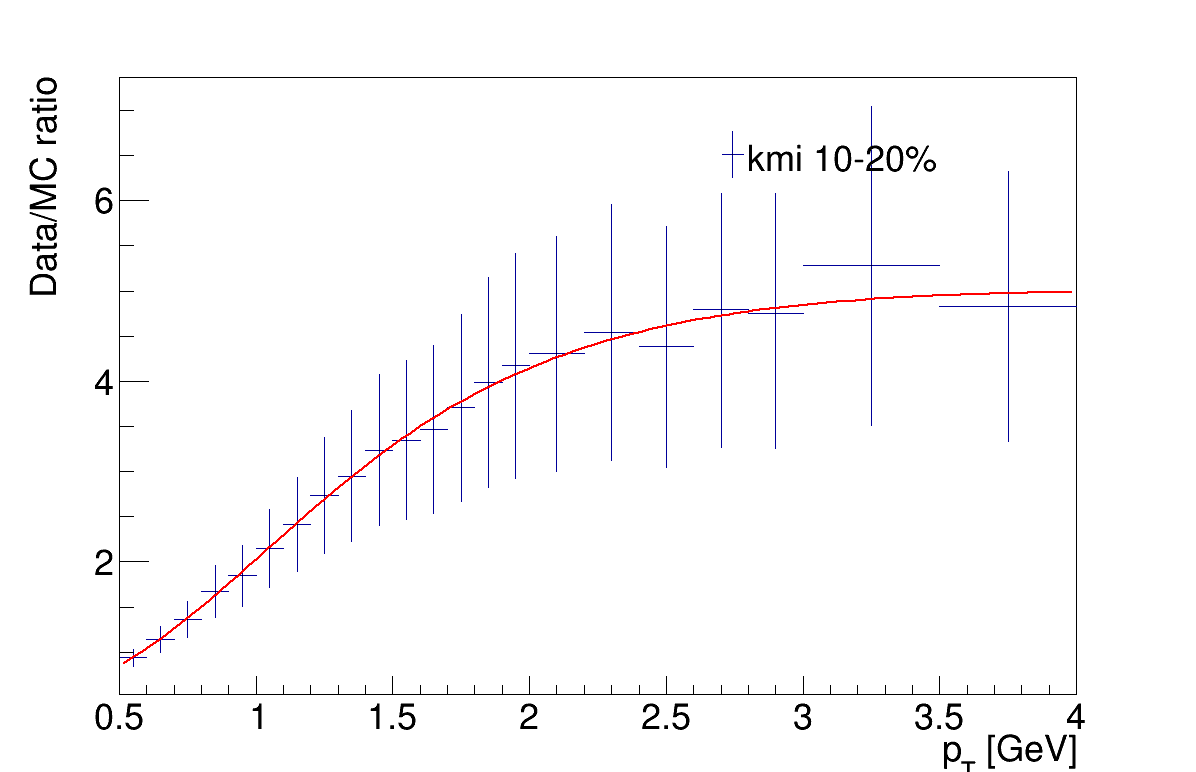
\includegraphics[width=0.24\linewidth]{detdeta/Figures/particle_reweighting_ratios/HIJING_kmi_1.png}
    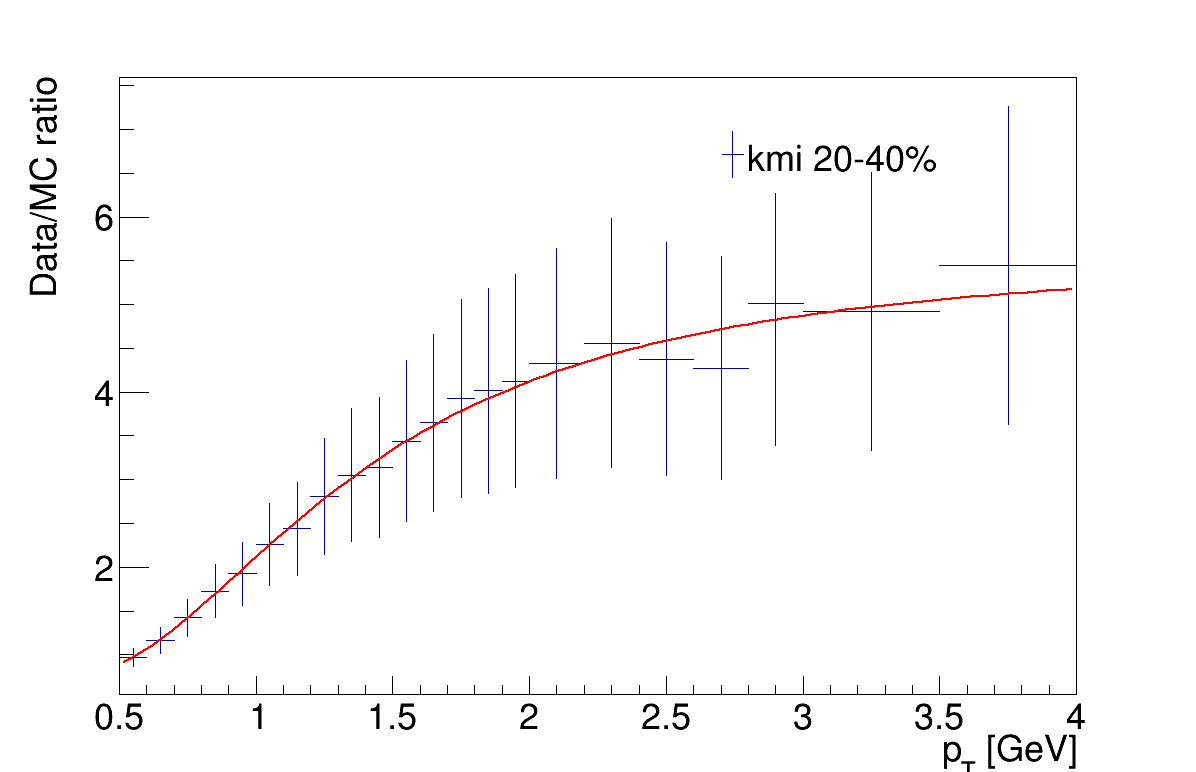
\includegraphics[width=0.24\linewidth]{detdeta/Figures/particle_reweighting_ratios/HIJING_kmi_2.png}
    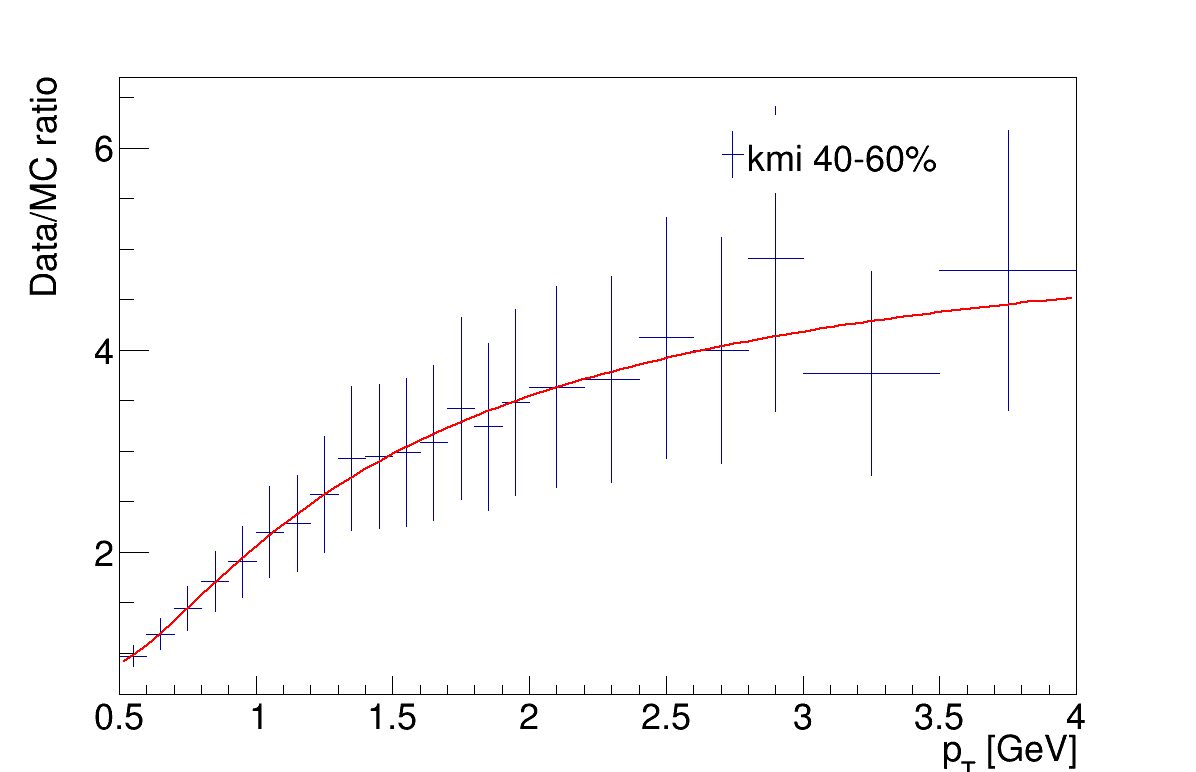
\includegraphics[width=0.24\linewidth]{detdeta/Figures/particle_reweighting_ratios/HIJING_kmi_3.png}
    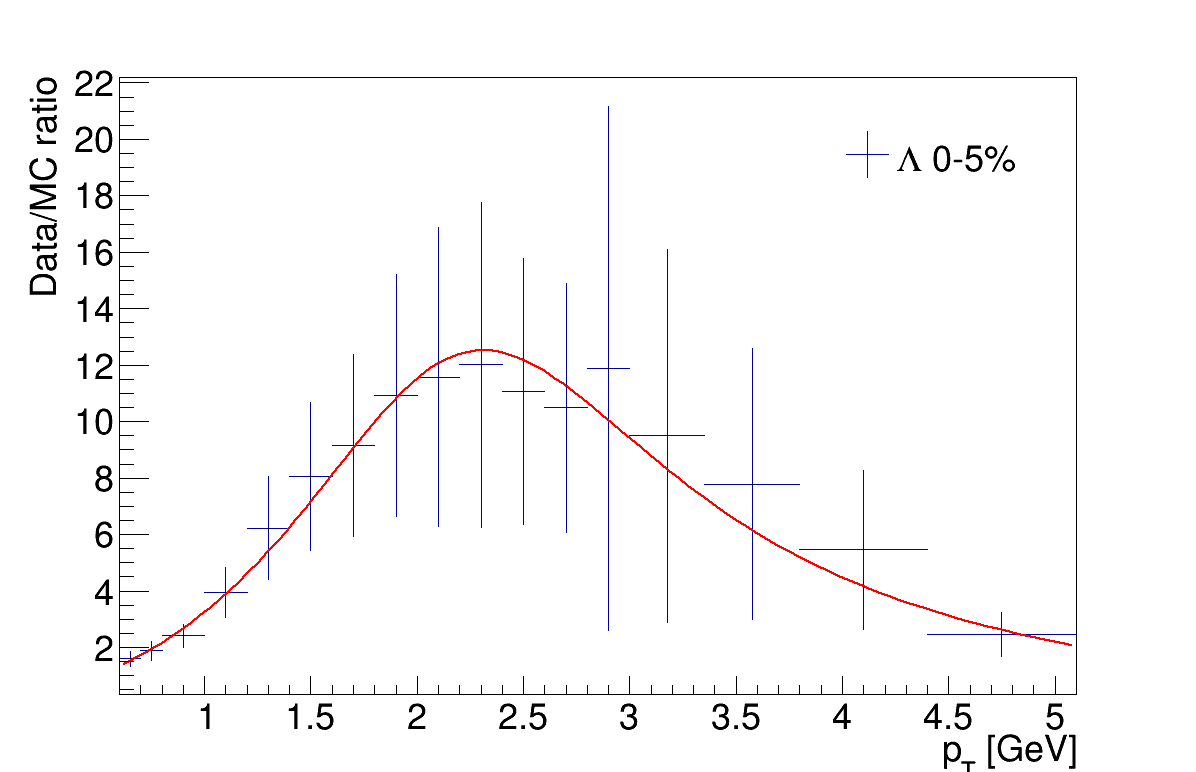
\includegraphics[width=0.24\linewidth]{detdeta/Figures/particle_reweighting_ratios/HIJING_lambda_0.png}
    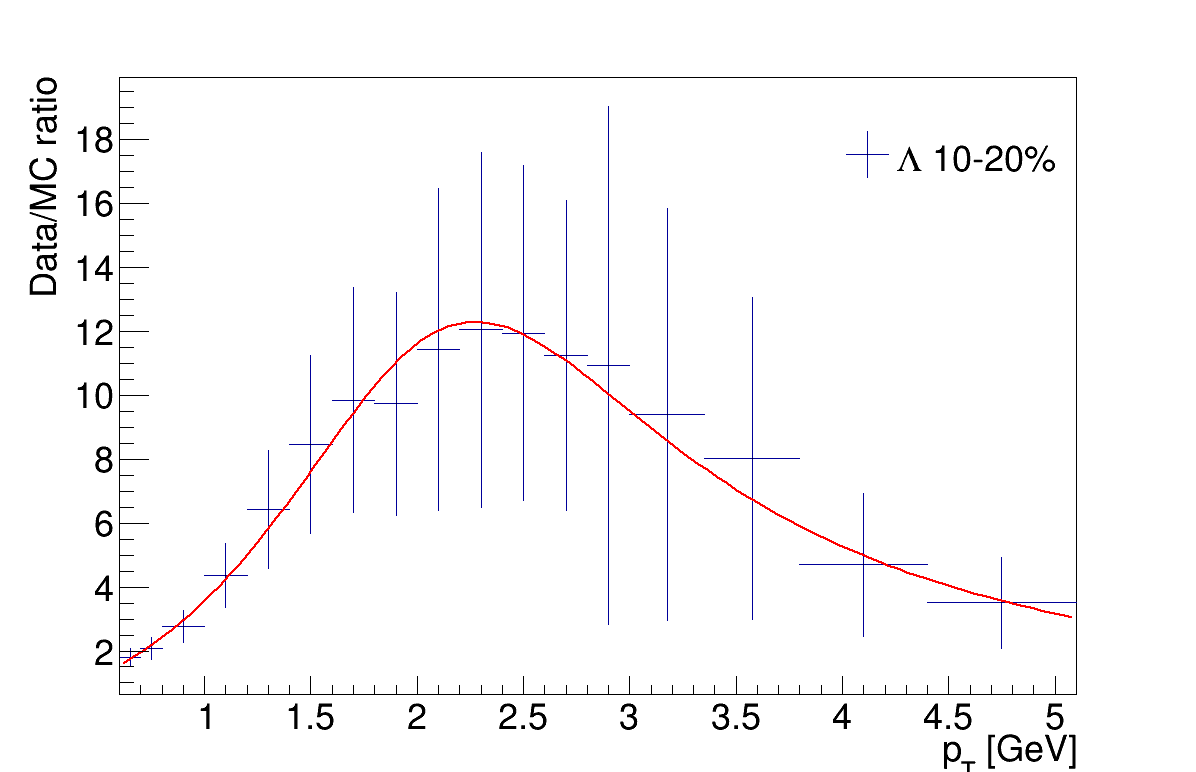
\includegraphics[width=0.24\linewidth]{detdeta/Figures/particle_reweighting_ratios/HIJING_lambda_1.png}
    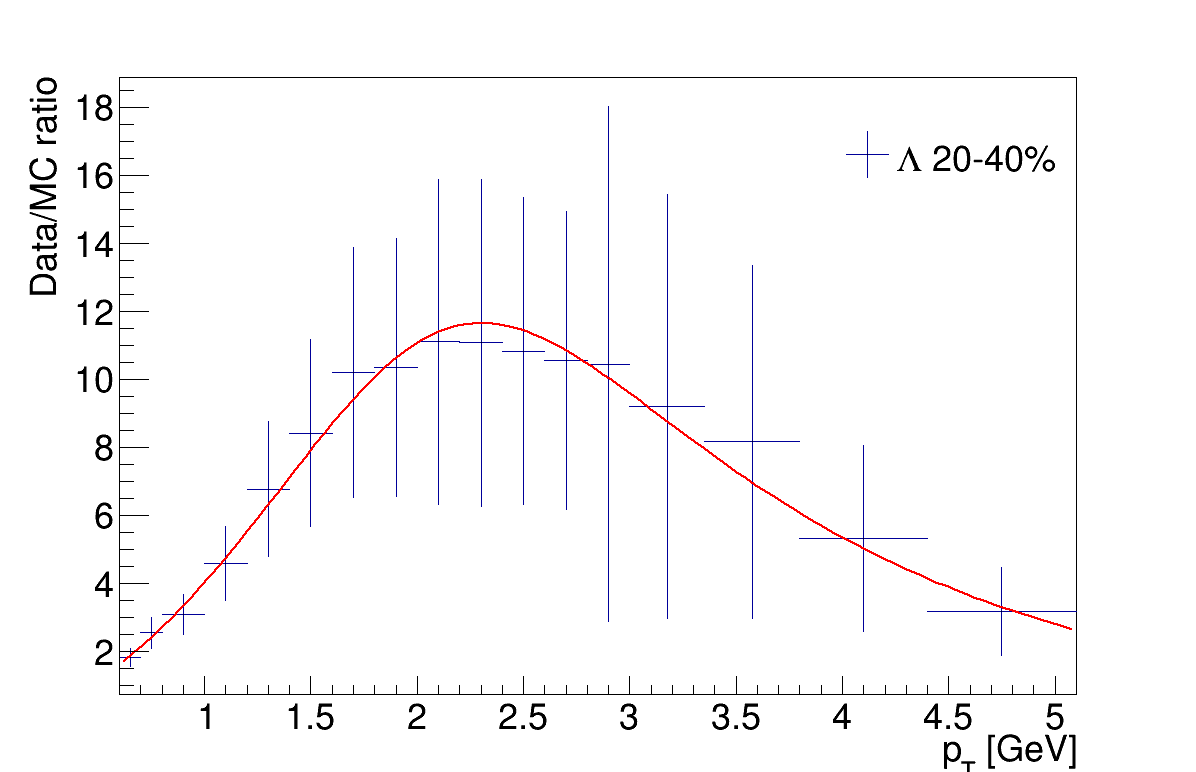
\includegraphics[width=0.24\linewidth]{detdeta/Figures/particle_reweighting_ratios/HIJING_lambda_2.png}
    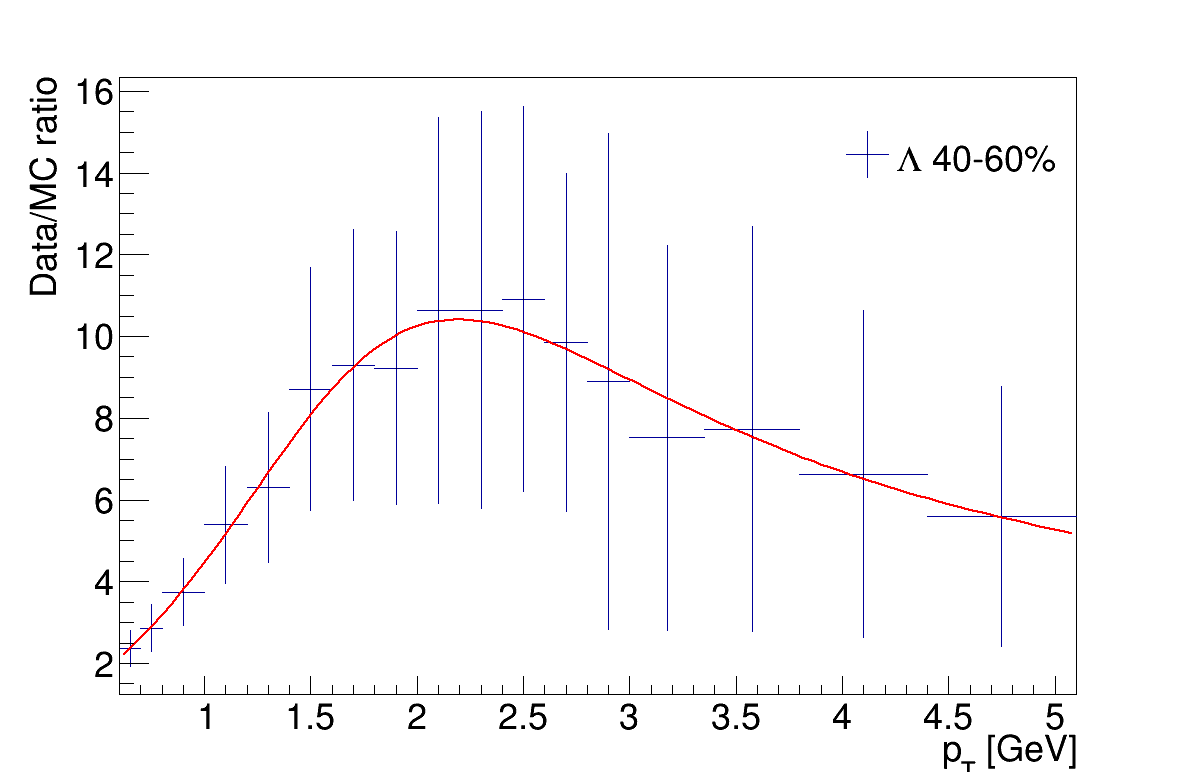
\includegraphics[width=0.24\linewidth]{detdeta/Figures/particle_reweighting_ratios/HIJING_lambda_3.png}
    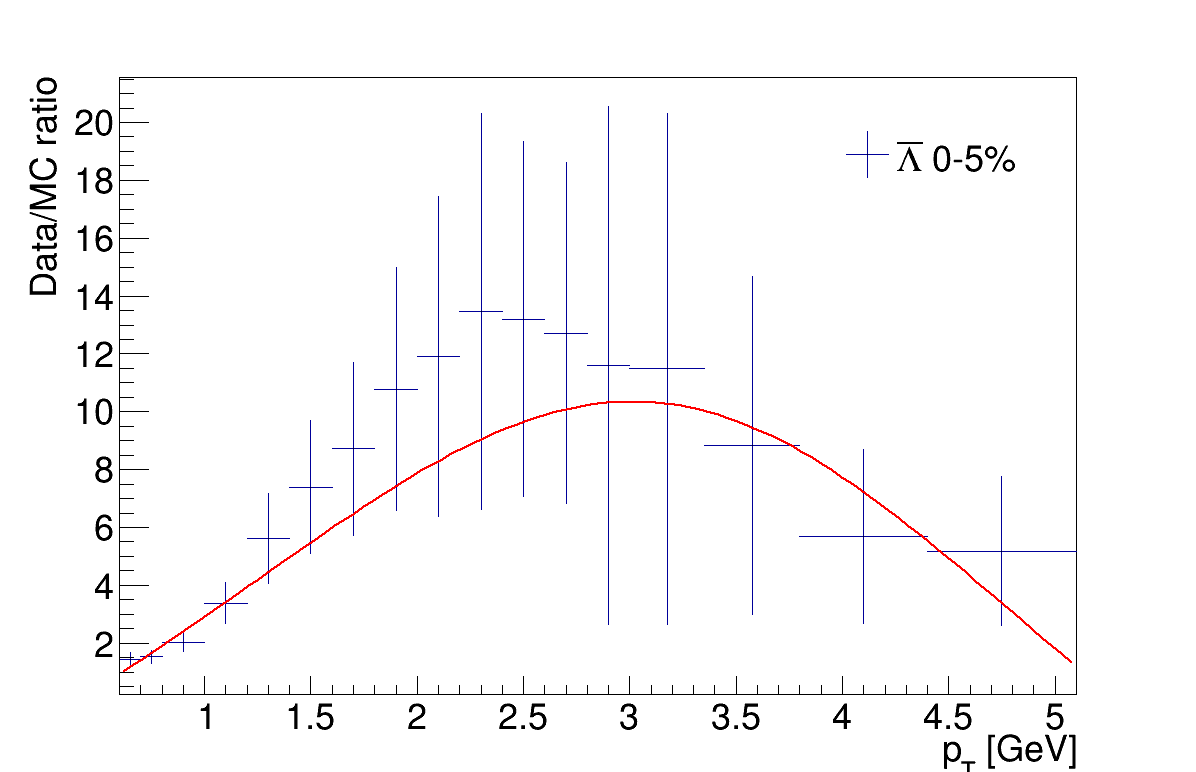
\includegraphics[width=0.24\linewidth]{detdeta/Figures/particle_reweighting_ratios/HIJING_lambda_bar_0.png}
    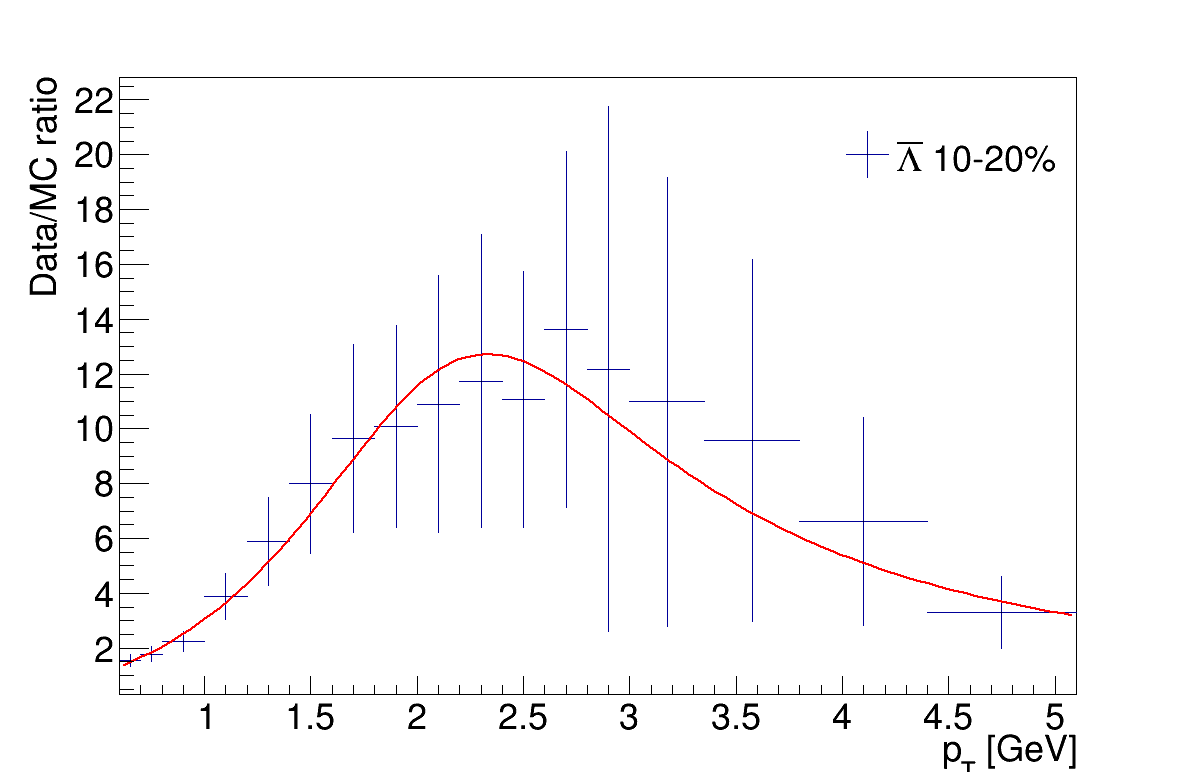
\includegraphics[width=0.24\linewidth]{detdeta/Figures/particle_reweighting_ratios/HIJING_lambda_bar_1.png}
    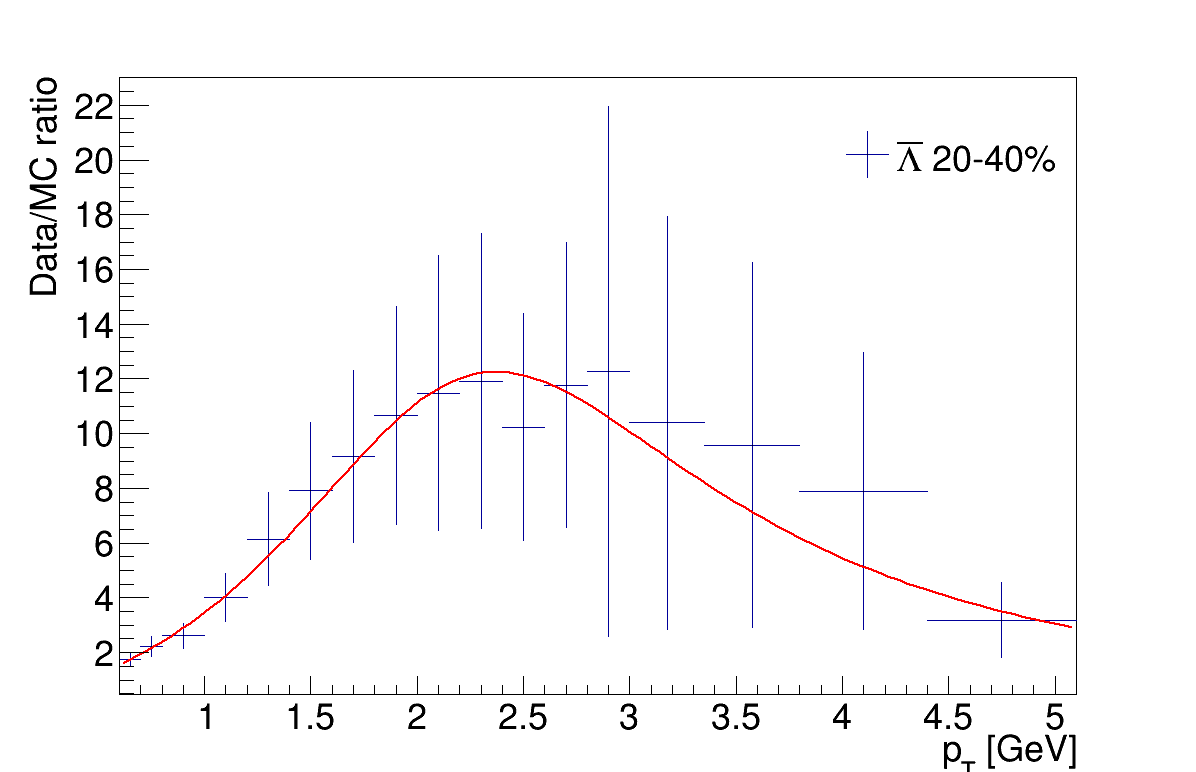
\includegraphics[width=0.24\linewidth]{detdeta/Figures/particle_reweighting_ratios/HIJING_lambda_bar_2.png}
    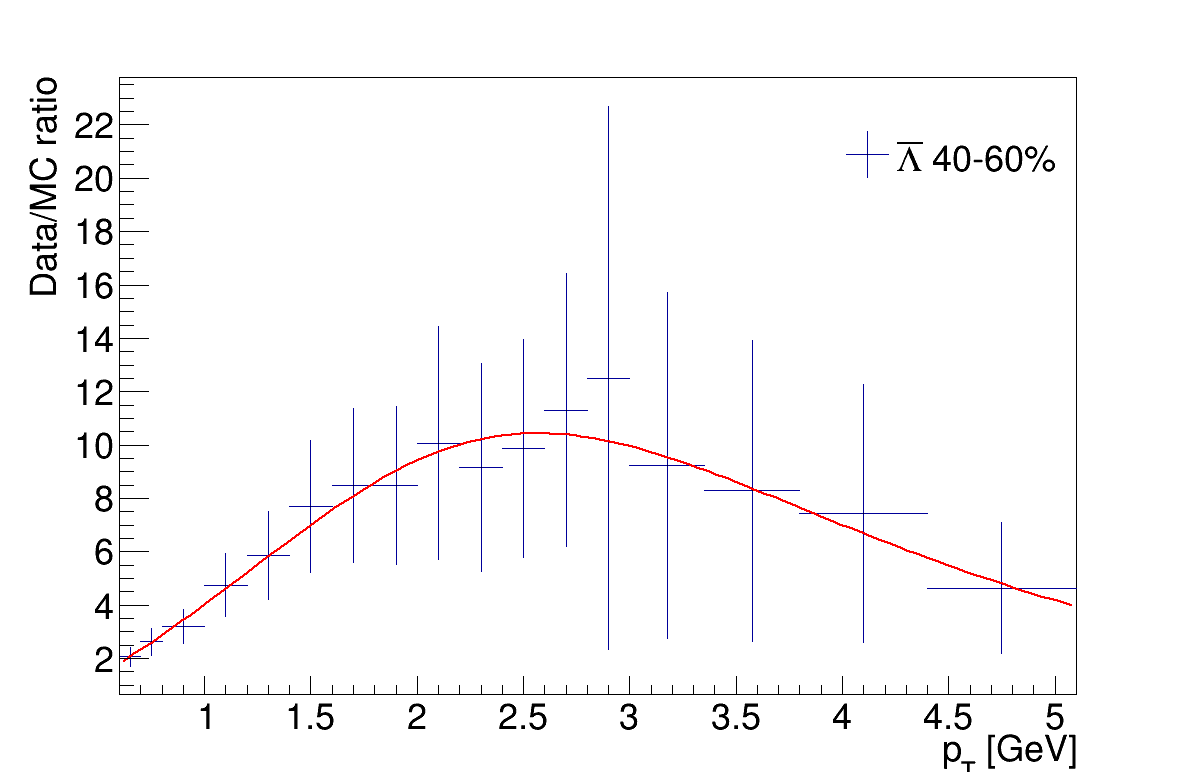
\includegraphics[width=0.24\linewidth]{detdeta/Figures/particle_reweighting_ratios/HIJING_lambda_bar_3.png}
    \caption{All data to MC ratios used in nominal HIJING reweighting method for protons, anti-protons, kaons, pions and lambda particles.}
    \label{fig:hijing_data_mc_particle_ratios}
\end{figure}

\begin{figure}
    \centering
    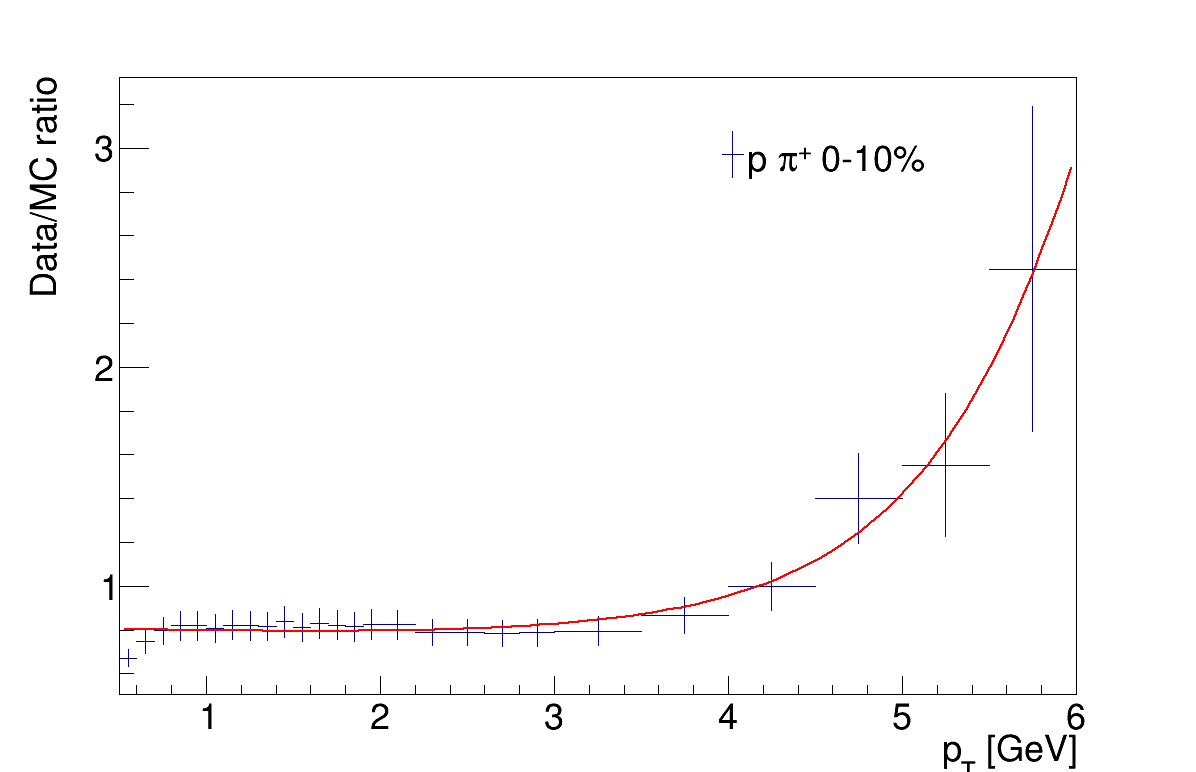
\includegraphics[width=0.24\linewidth]{detdeta/Figures/particle_reweighting_ratios/EPOS_p_0.png}
    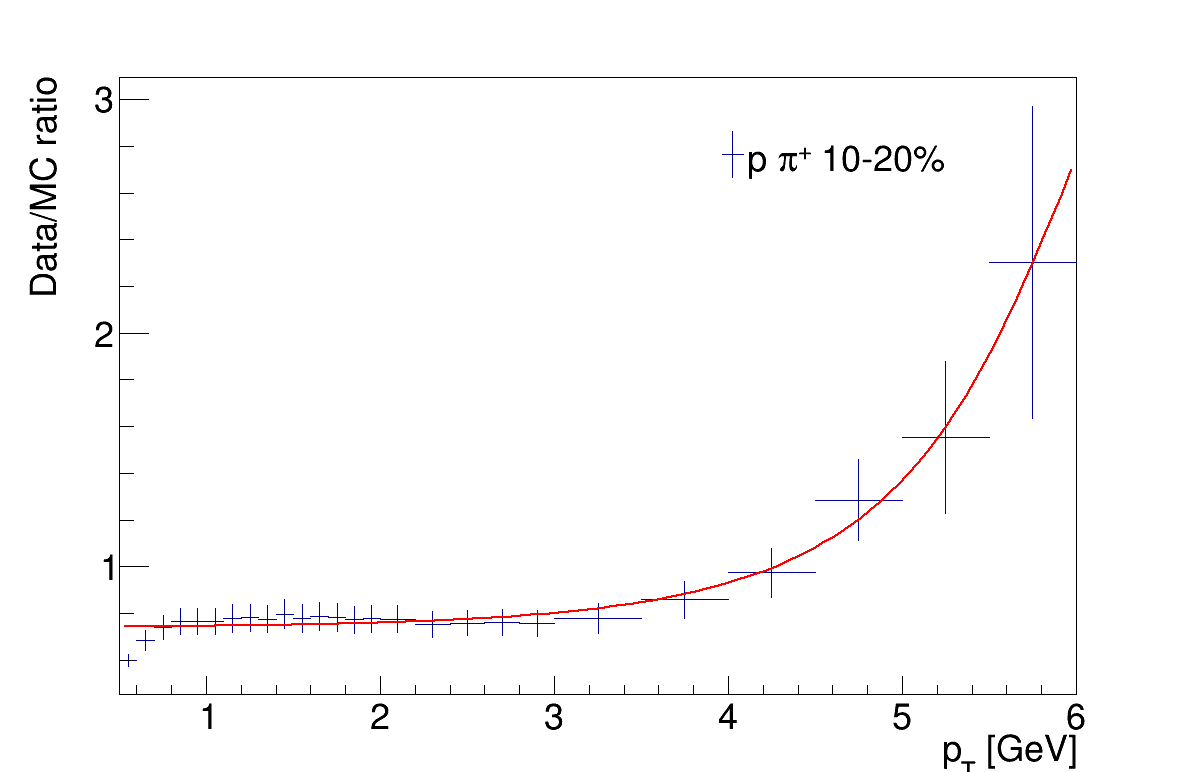
\includegraphics[width=0.24\linewidth]{detdeta/Figures/particle_reweighting_ratios/EPOS_p_1.png}
    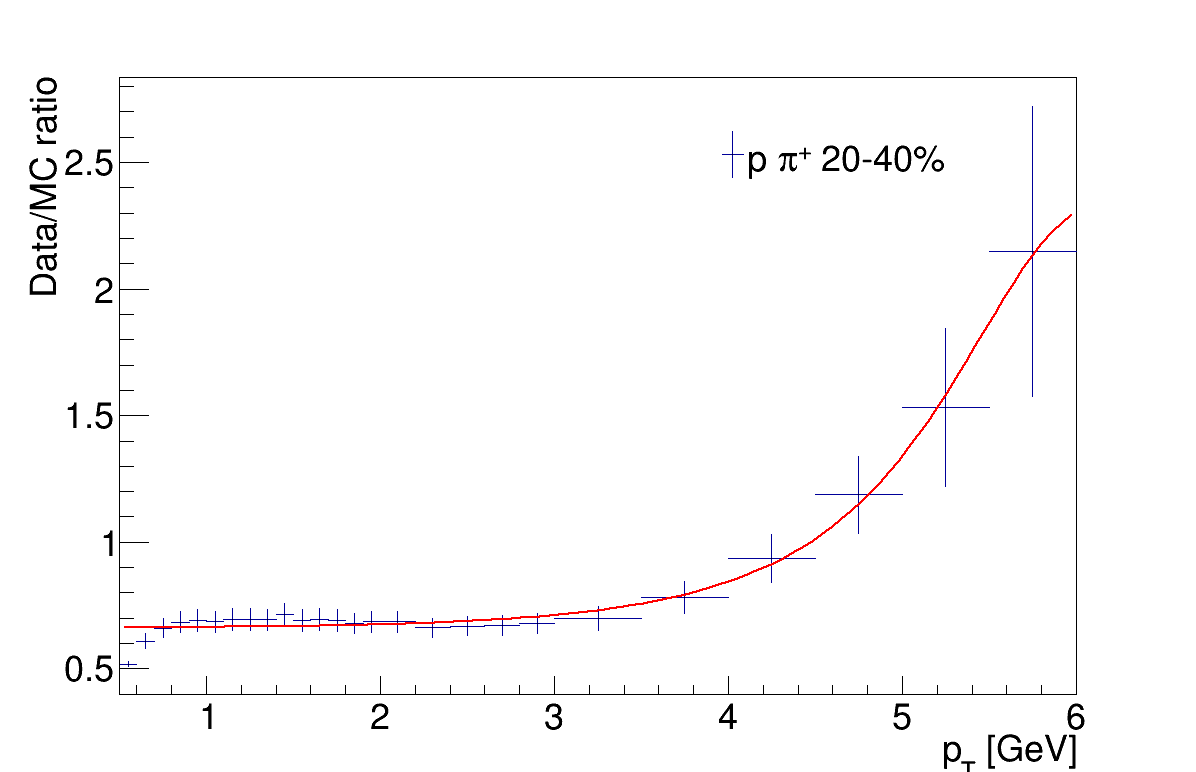
\includegraphics[width=0.24\linewidth]{detdeta/Figures/particle_reweighting_ratios/EPOS_p_2.png}
    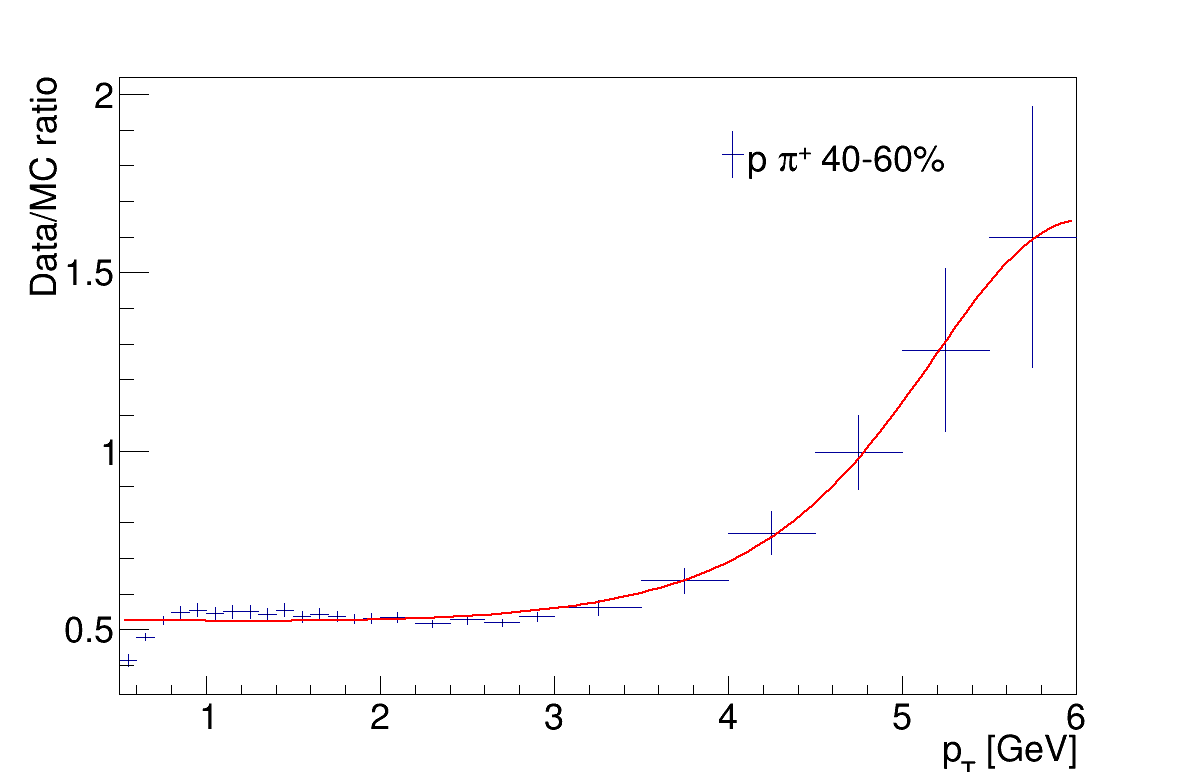
\includegraphics[width=0.24\linewidth]{detdeta/Figures/particle_reweighting_ratios/EPOS_p_3.png}
    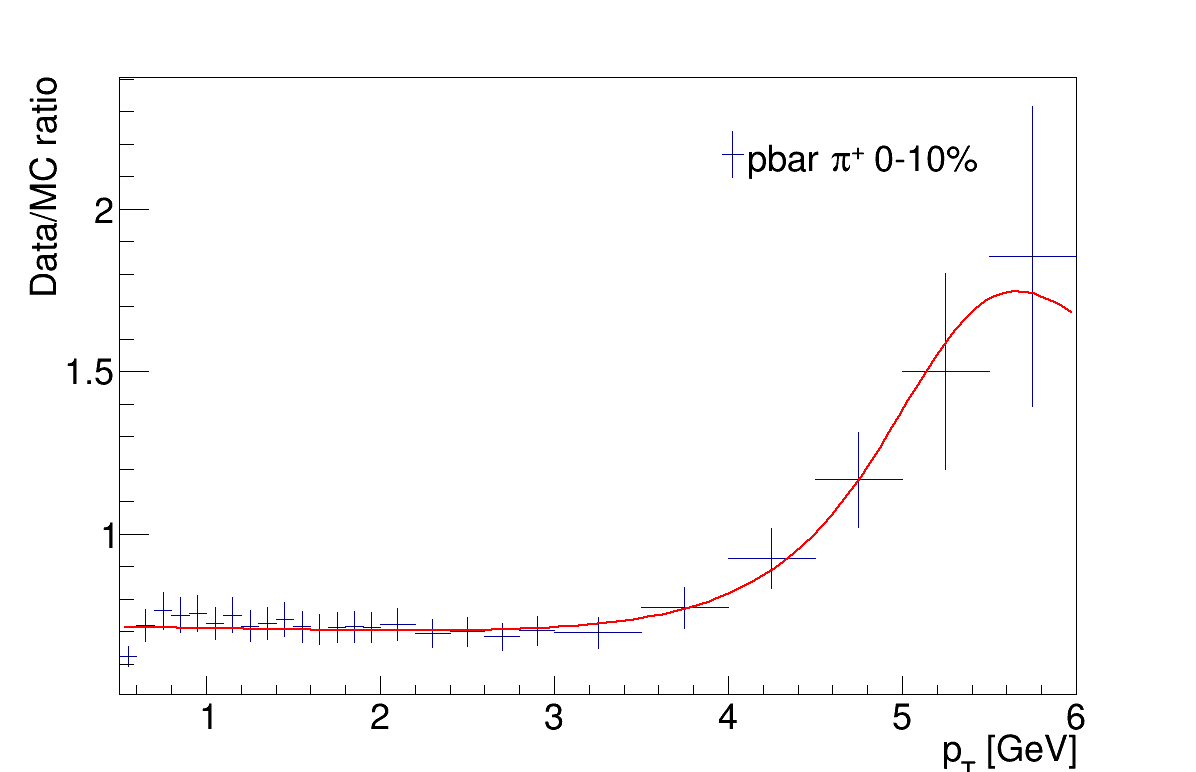
\includegraphics[width=0.24\linewidth]{detdeta/Figures/particle_reweighting_ratios/EPOS_pbar_0.png}
    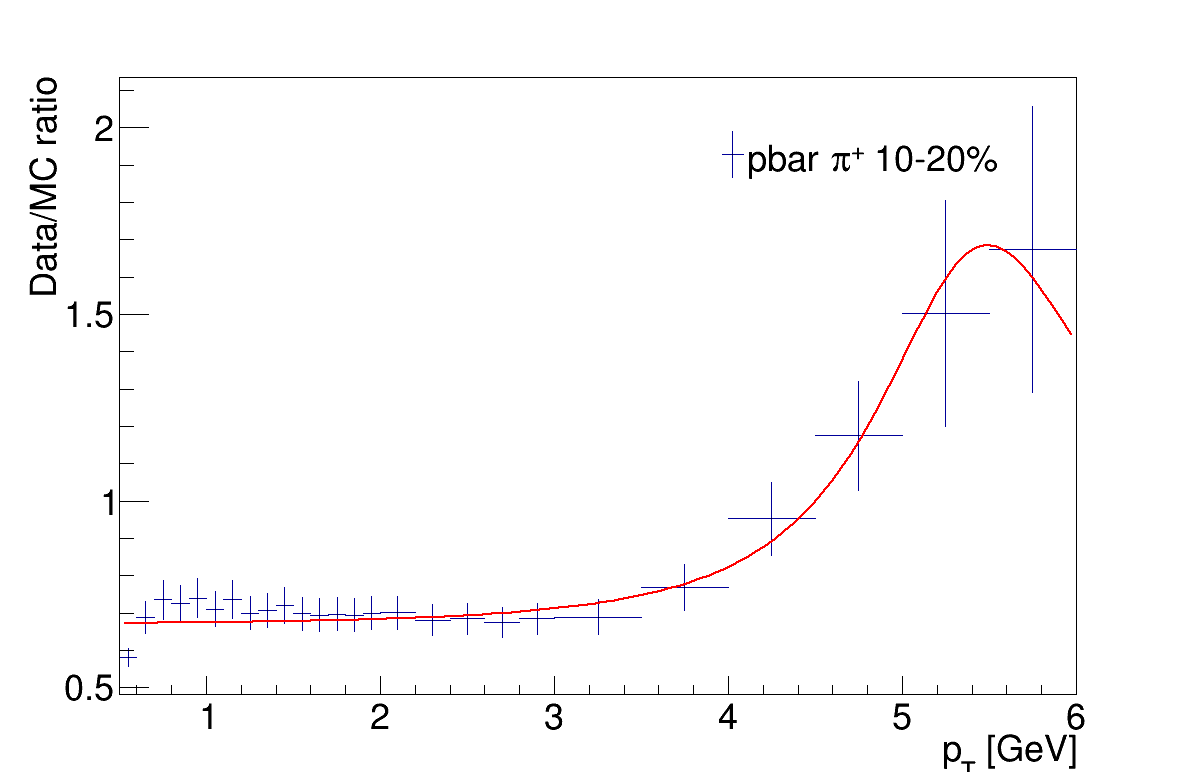
\includegraphics[width=0.24\linewidth]{detdeta/Figures/particle_reweighting_ratios/EPOS_pbar_1.png}
    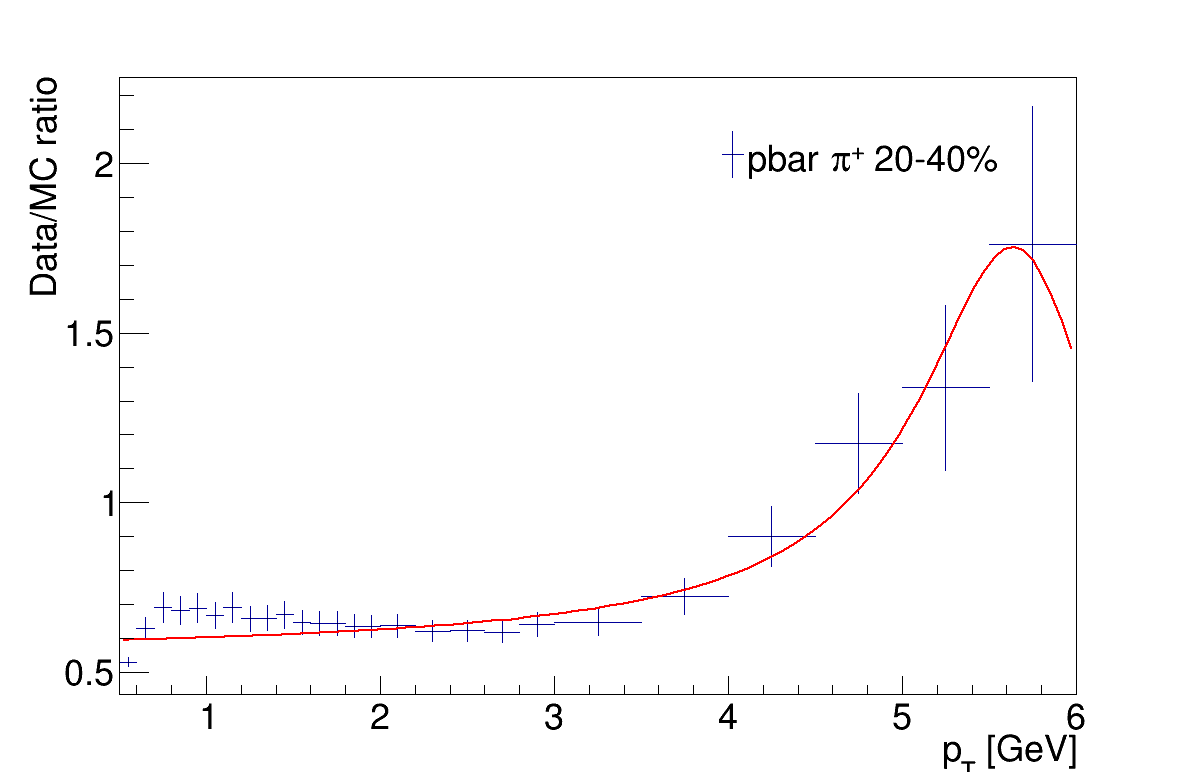
\includegraphics[width=0.24\linewidth]{detdeta/Figures/particle_reweighting_ratios/EPOS_pbar_2.png}
    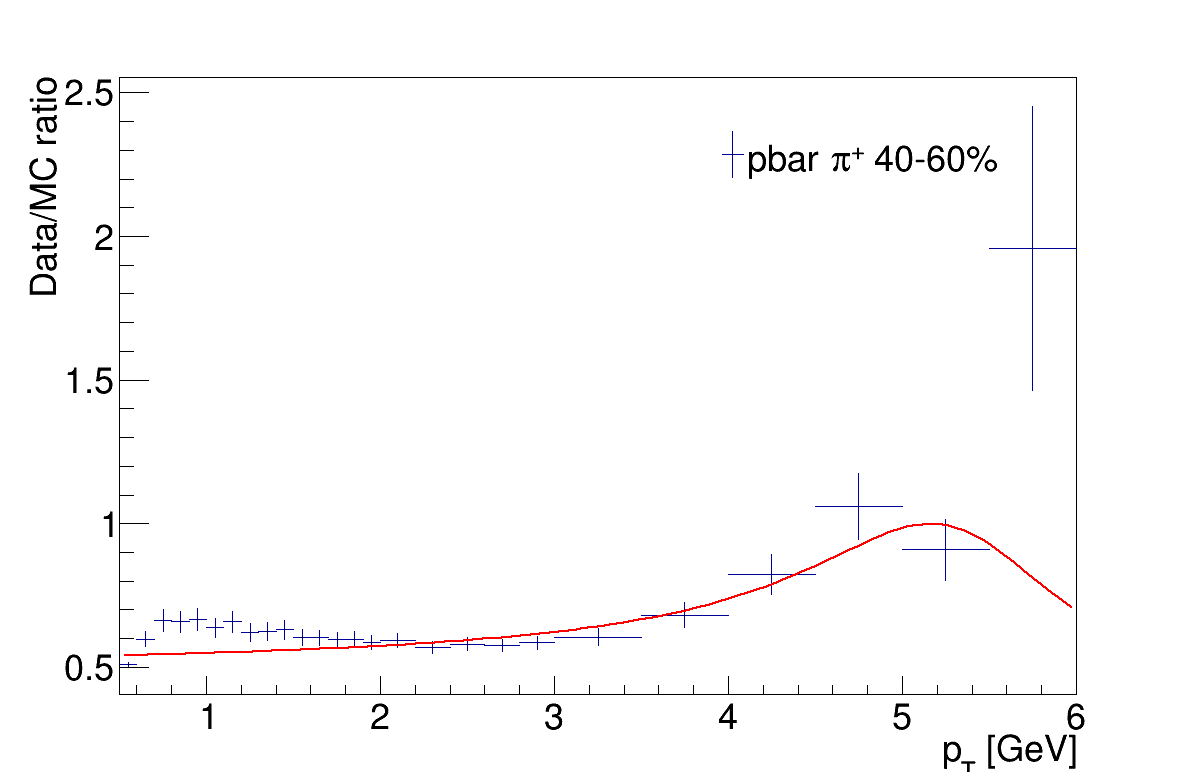
\includegraphics[width=0.24\linewidth]{detdeta/Figures/particle_reweighting_ratios/EPOS_pbar_3.png}
    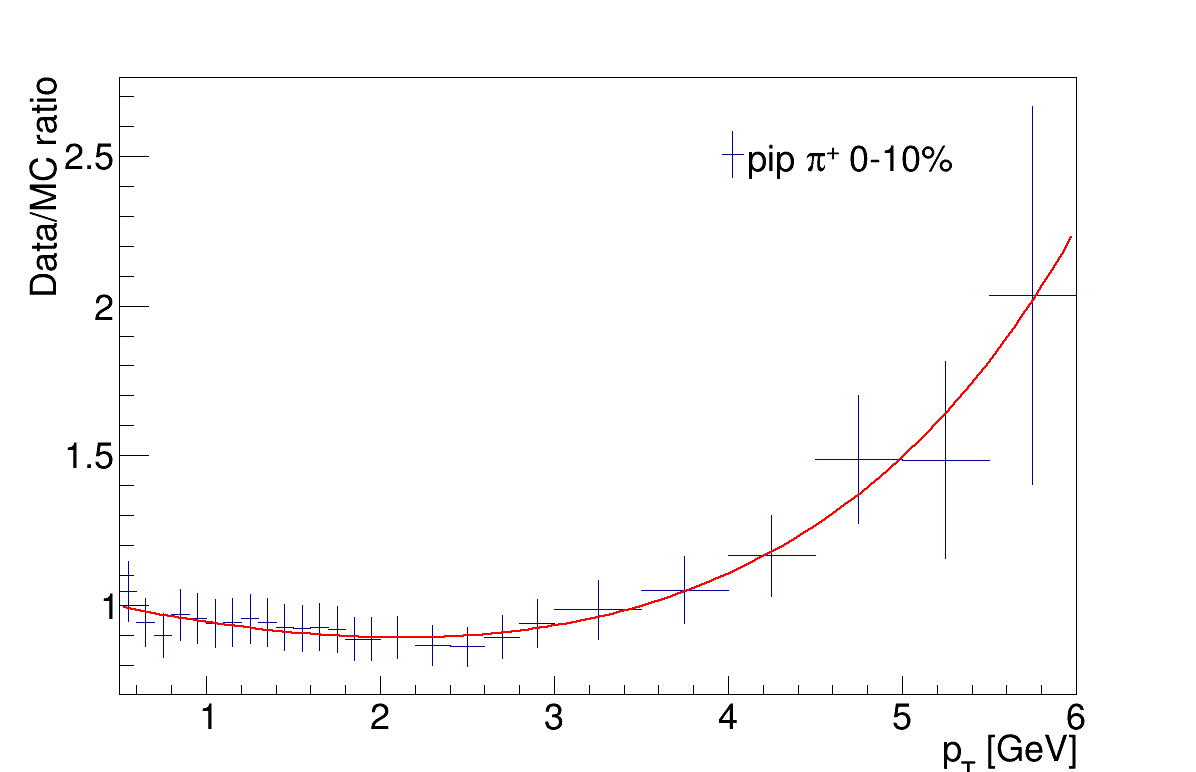
\includegraphics[width=0.24\linewidth]{detdeta/Figures/particle_reweighting_ratios/EPOS_pip_0.png}
    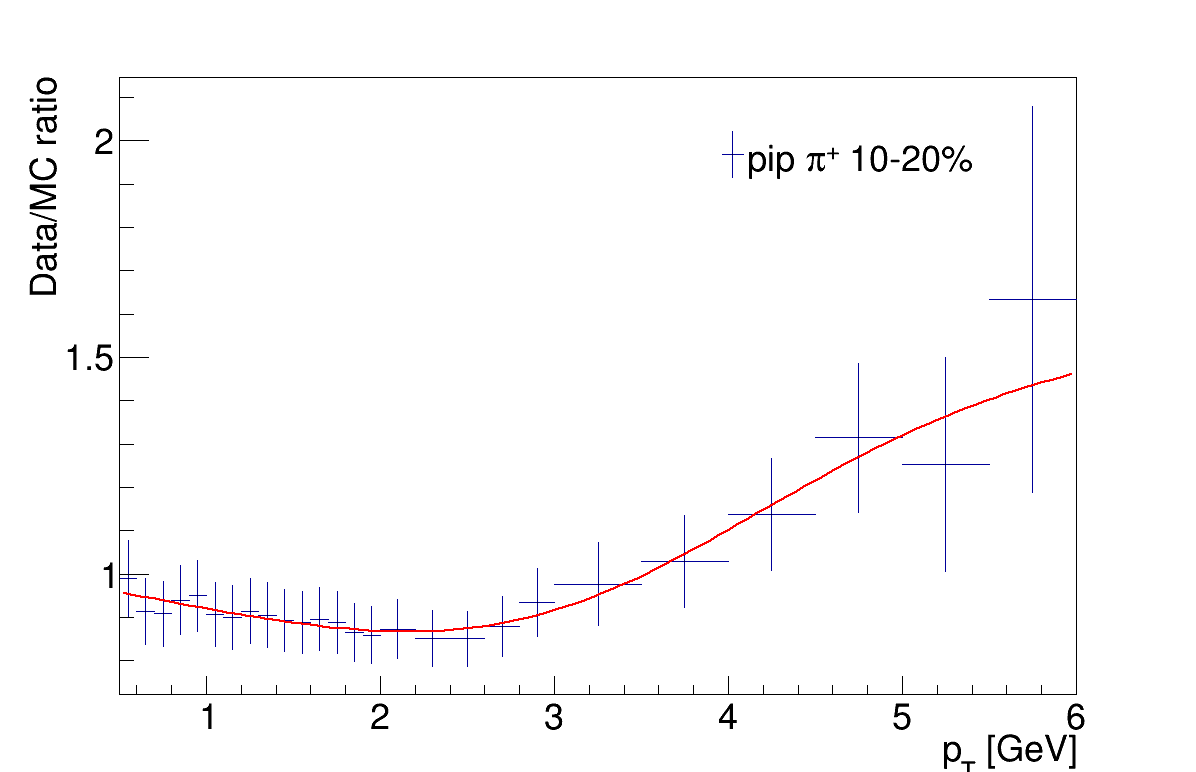
\includegraphics[width=0.24\linewidth]{detdeta/Figures/particle_reweighting_ratios/EPOS_pip_1.png}
    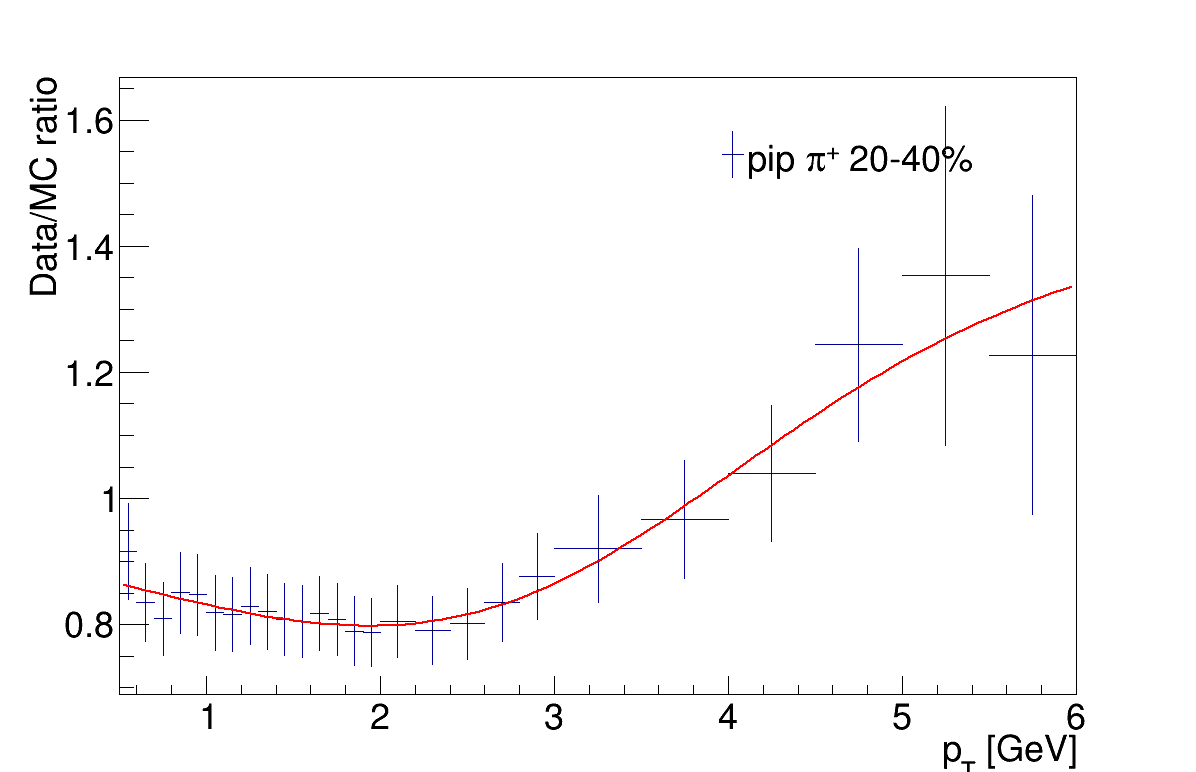
\includegraphics[width=0.24\linewidth]{detdeta/Figures/particle_reweighting_ratios/EPOS_pip_2.png}
    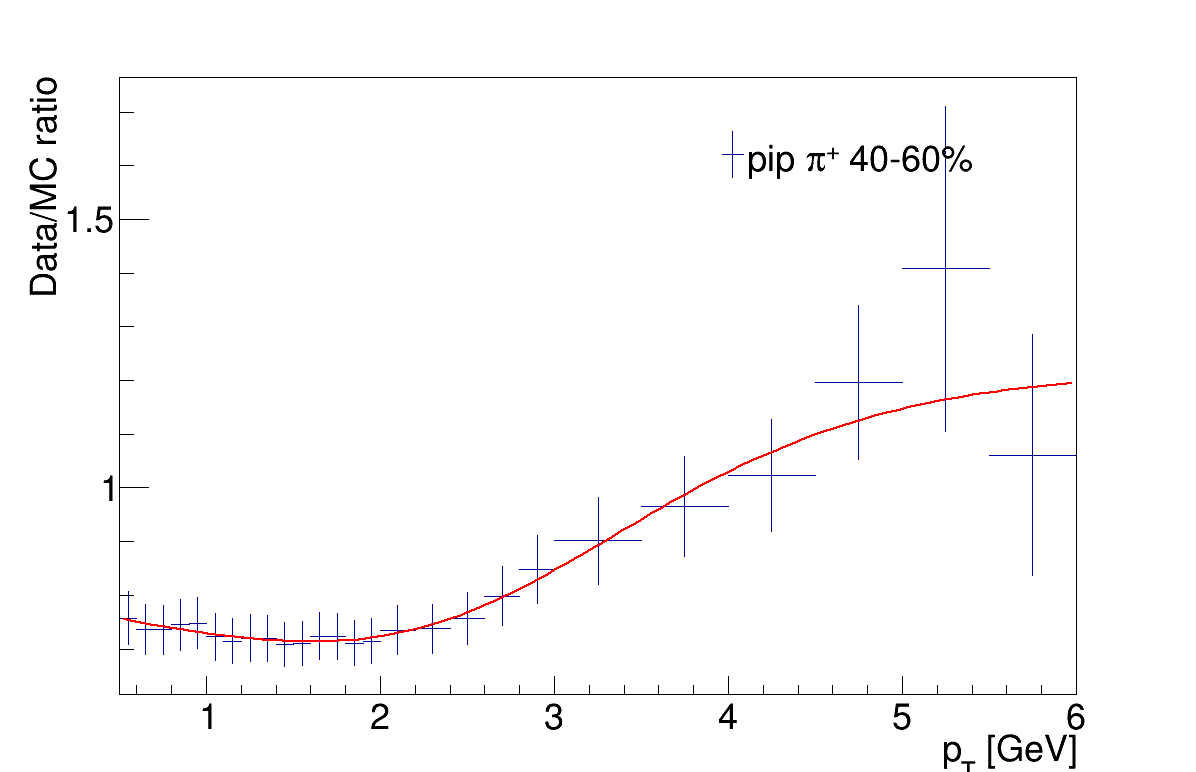
\includegraphics[width=0.24\linewidth]{detdeta/Figures/particle_reweighting_ratios/EPOS_pip_3.png}
    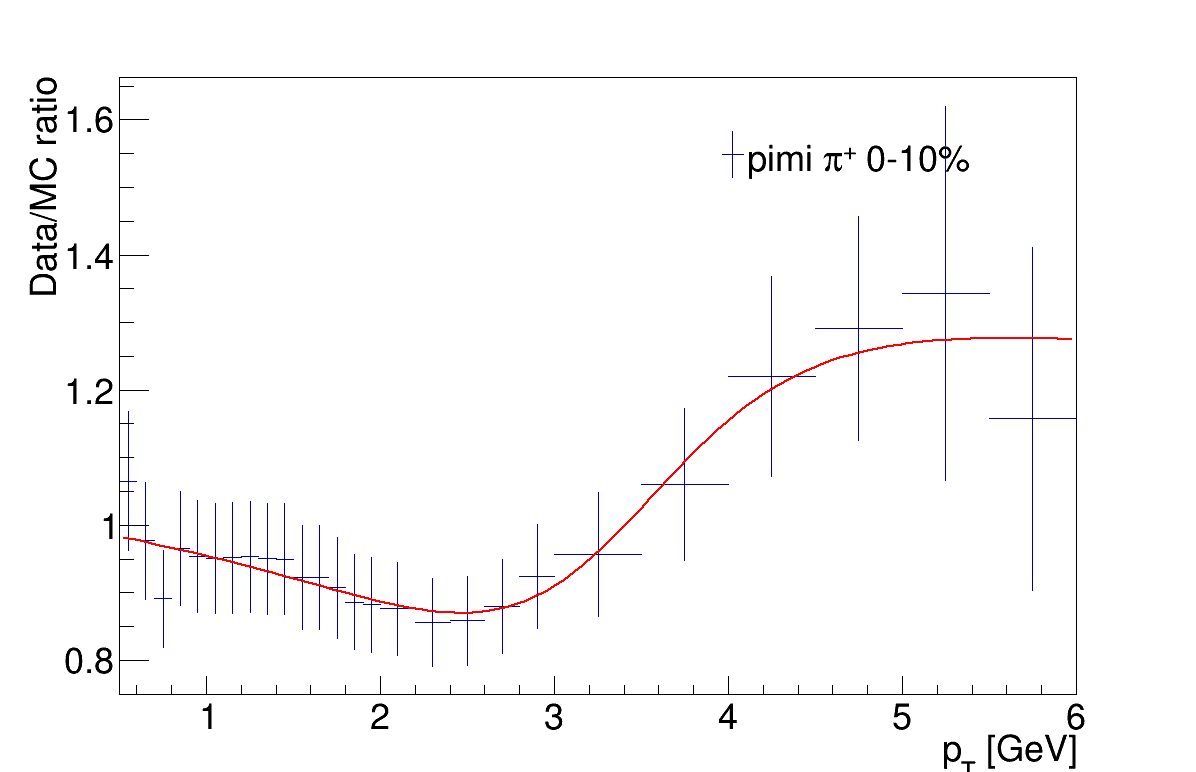
\includegraphics[width=0.24\linewidth]{detdeta/Figures/particle_reweighting_ratios/EPOS_pimi_0.png}
    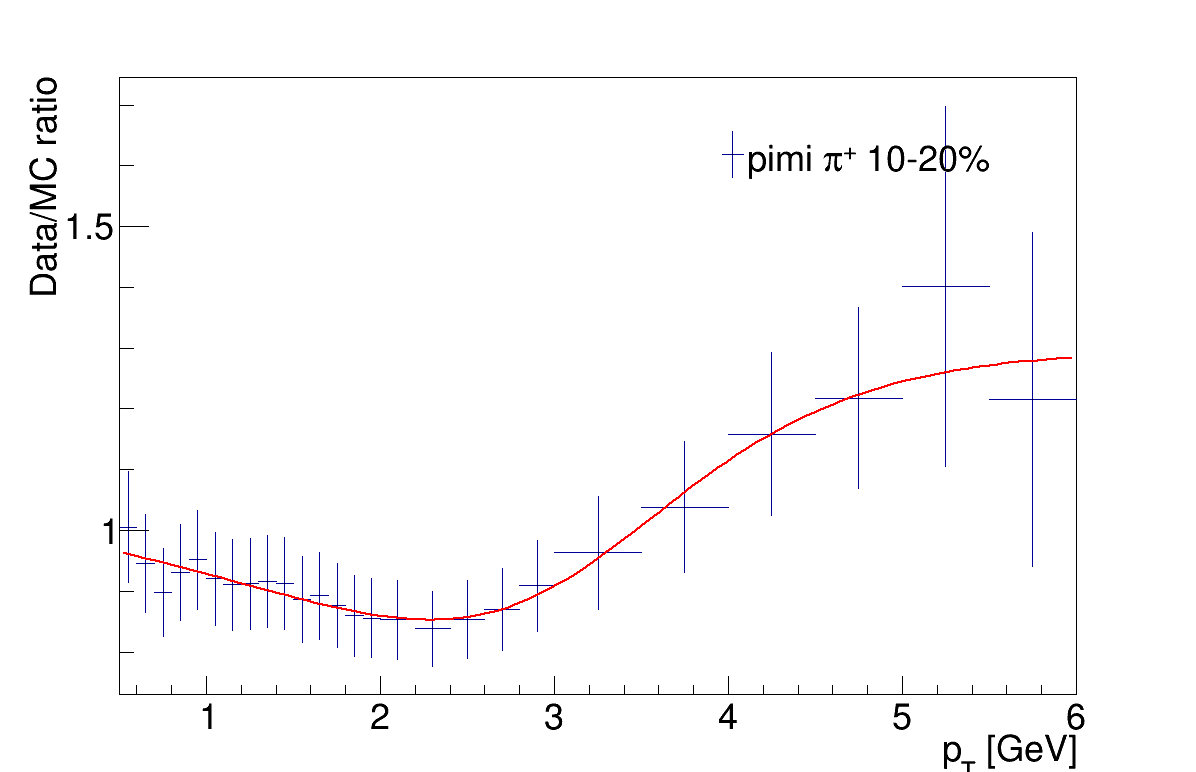
\includegraphics[width=0.24\linewidth]{detdeta/Figures/particle_reweighting_ratios/EPOS_pimi_1.png}
    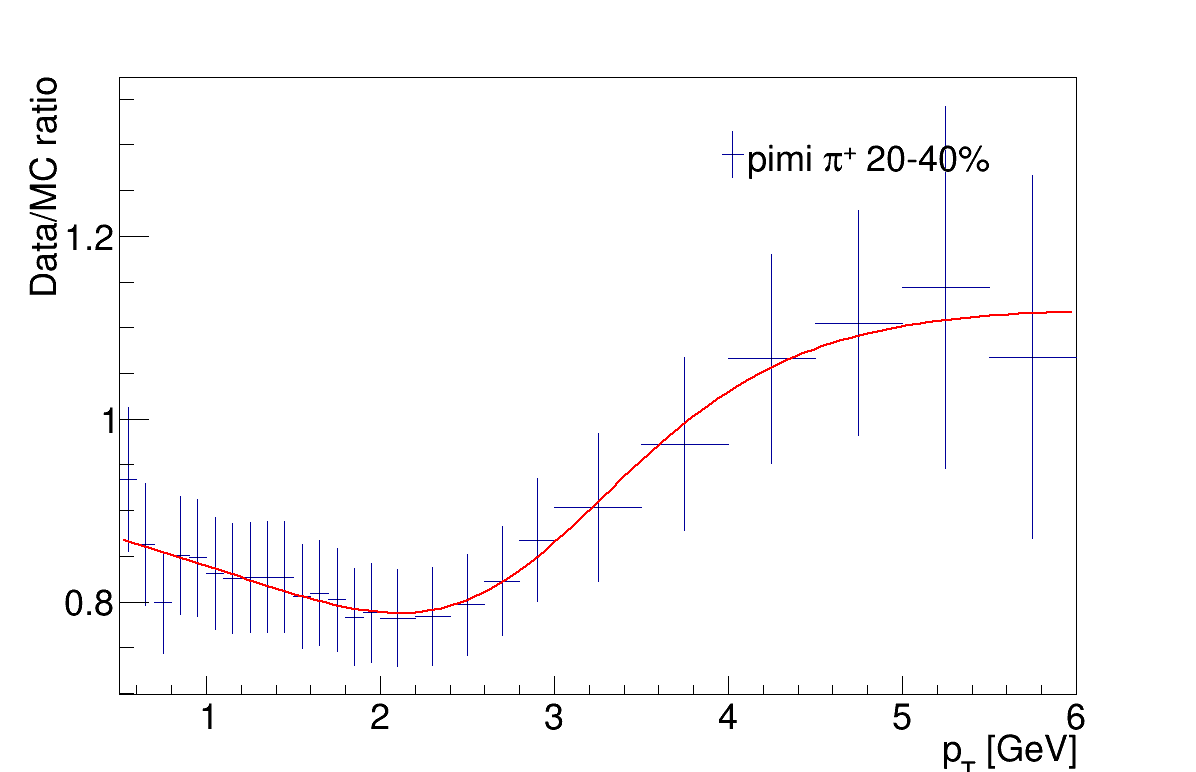
\includegraphics[width=0.24\linewidth]{detdeta/Figures/particle_reweighting_ratios/EPOS_pimi_2.png}
    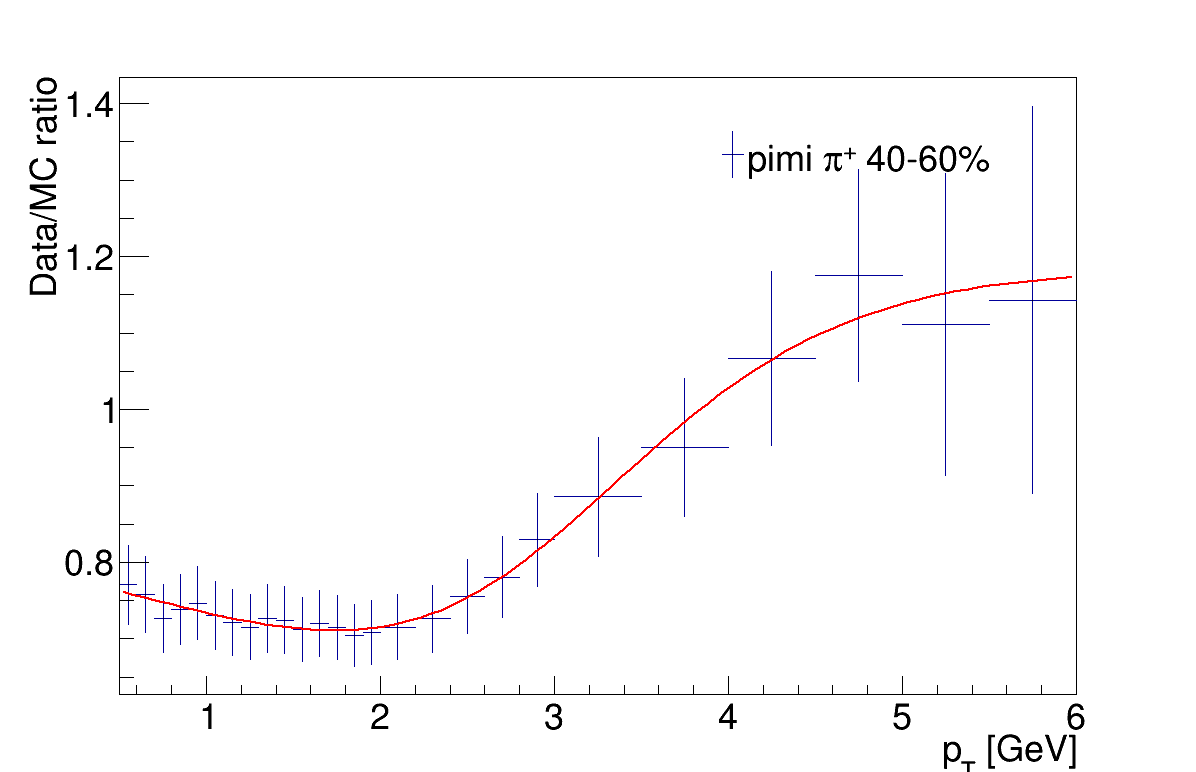
\includegraphics[width=0.24\linewidth]{detdeta/Figures/particle_reweighting_ratios/EPOS_pimi_3.png}
    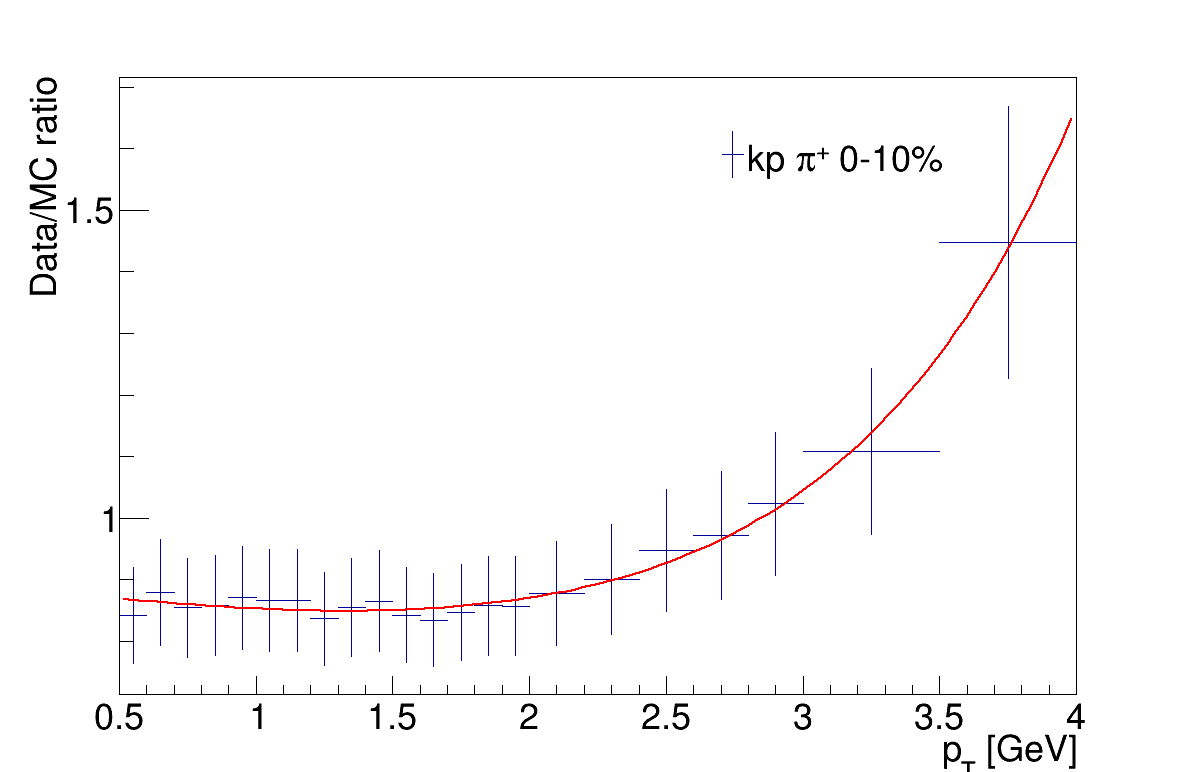
\includegraphics[width=0.24\linewidth]{detdeta/Figures/particle_reweighting_ratios/EPOS_kp_0.png}
    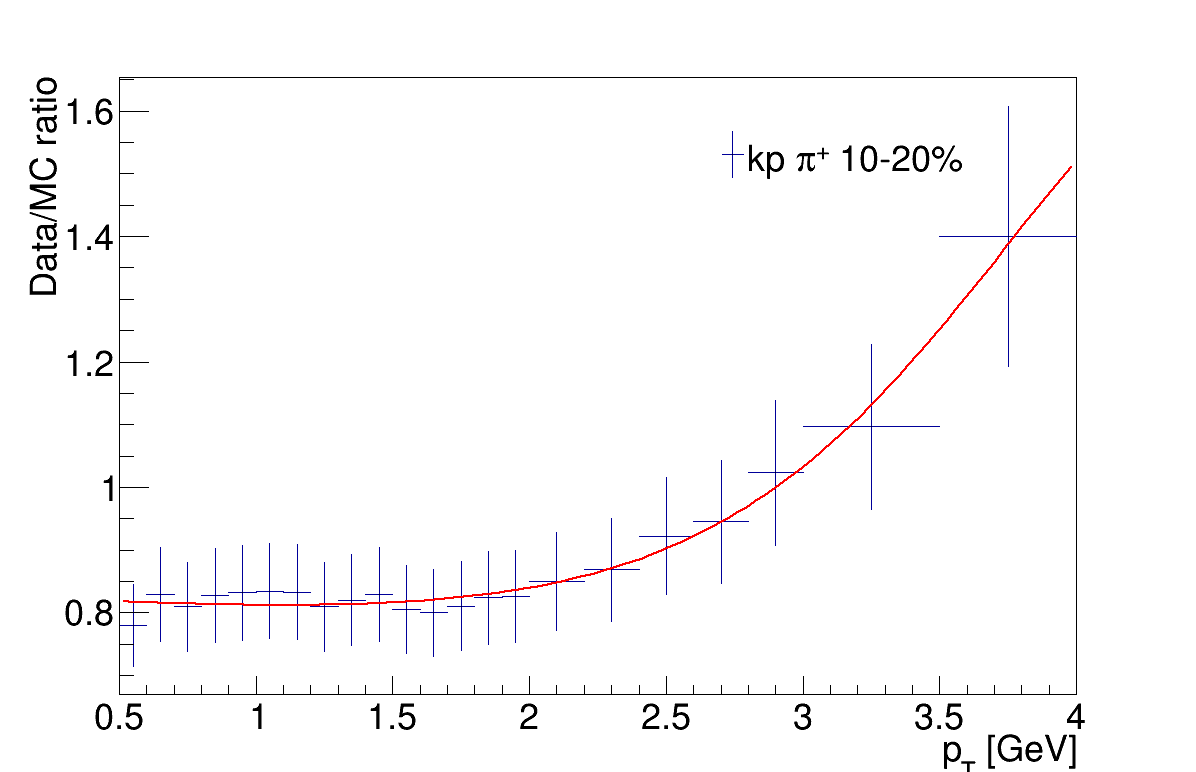
\includegraphics[width=0.24\linewidth]{detdeta/Figures/particle_reweighting_ratios/EPOS_kp_1.png}
    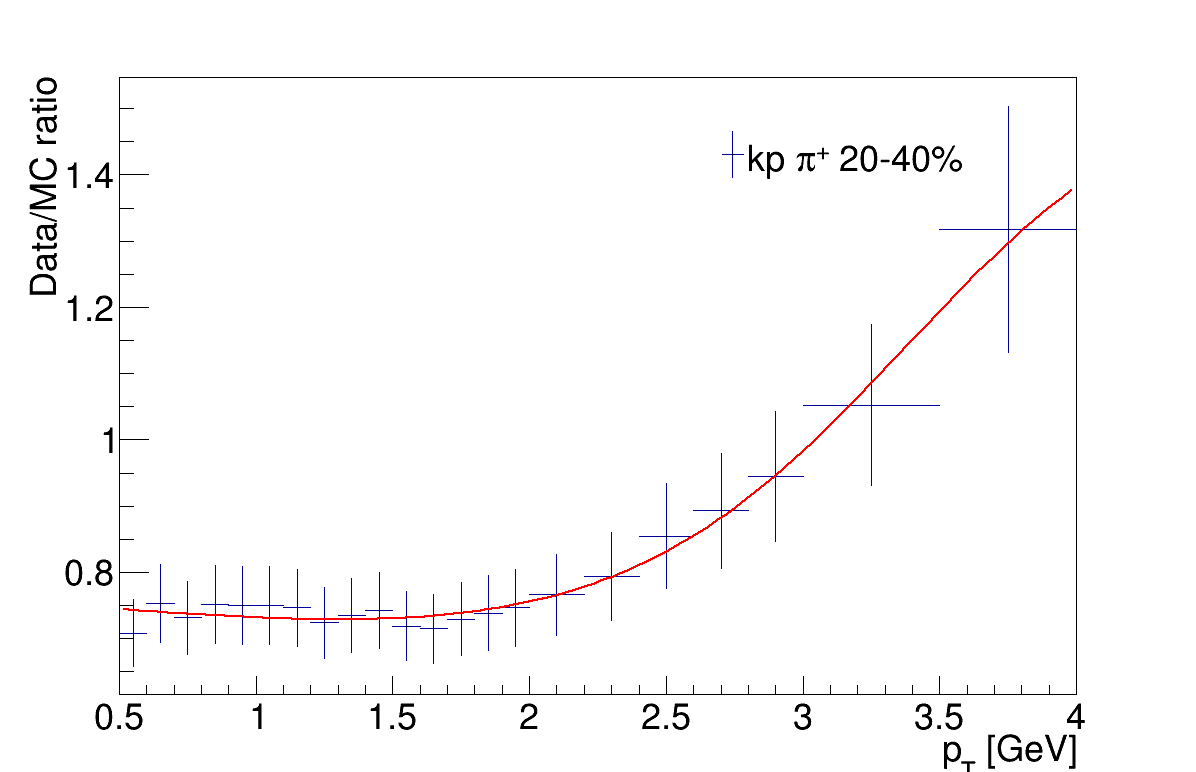
\includegraphics[width=0.24\linewidth]{detdeta/Figures/particle_reweighting_ratios/EPOS_kp_2.png}
    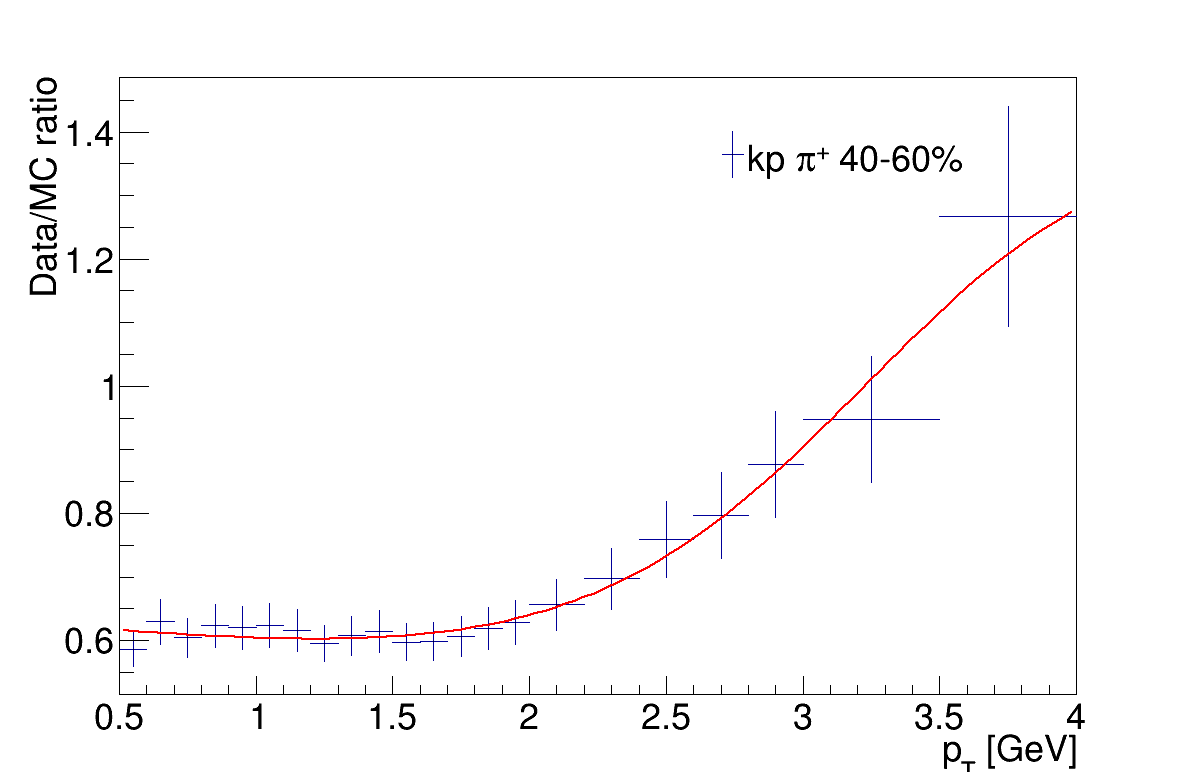
\includegraphics[width=0.24\linewidth]{detdeta/Figures/particle_reweighting_ratios/EPOS_kp_3.png}
    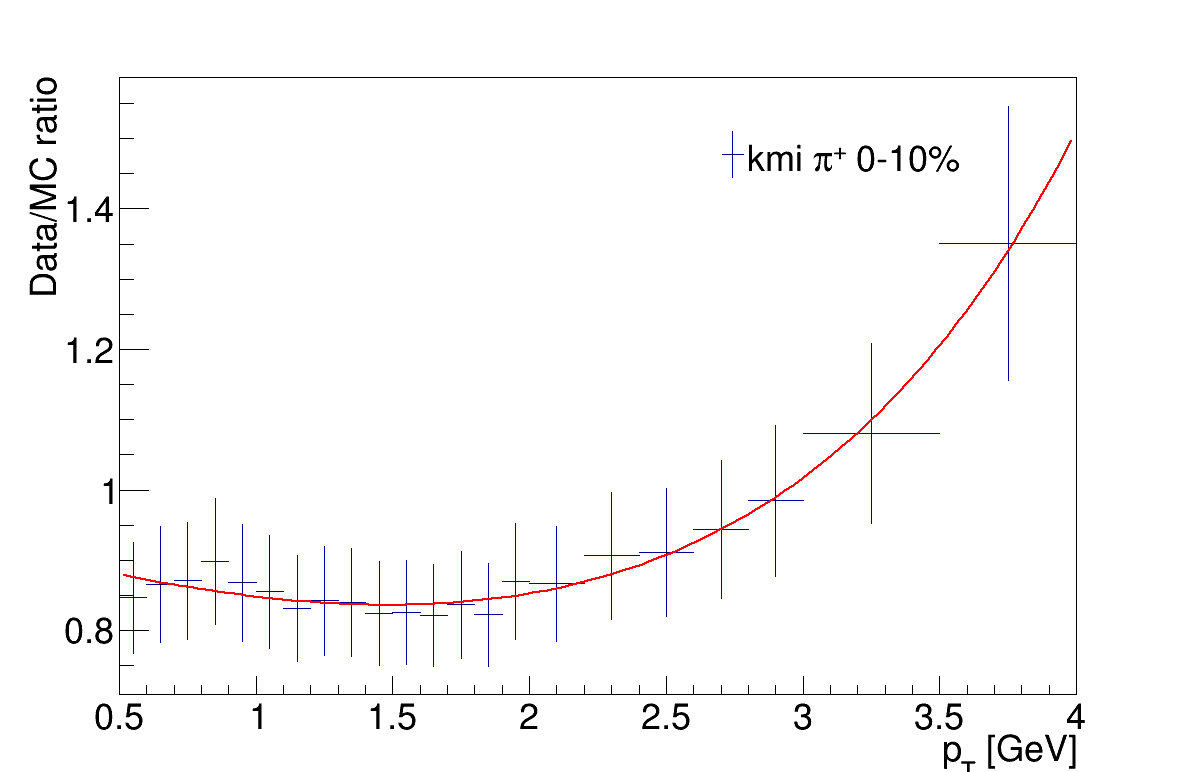
\includegraphics[width=0.24\linewidth]{detdeta/Figures/particle_reweighting_ratios/EPOS_kmi_0.png}
    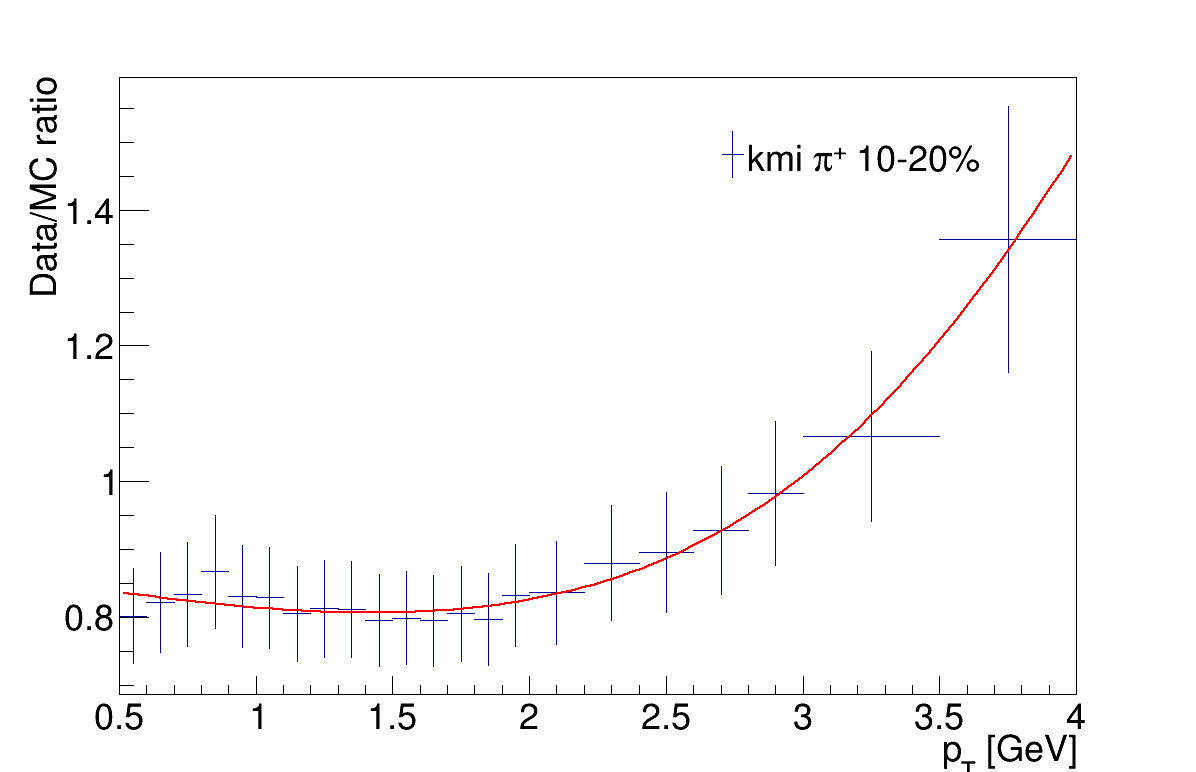
\includegraphics[width=0.24\linewidth]{detdeta/Figures/particle_reweighting_ratios/EPOS_kmi_1.png}
    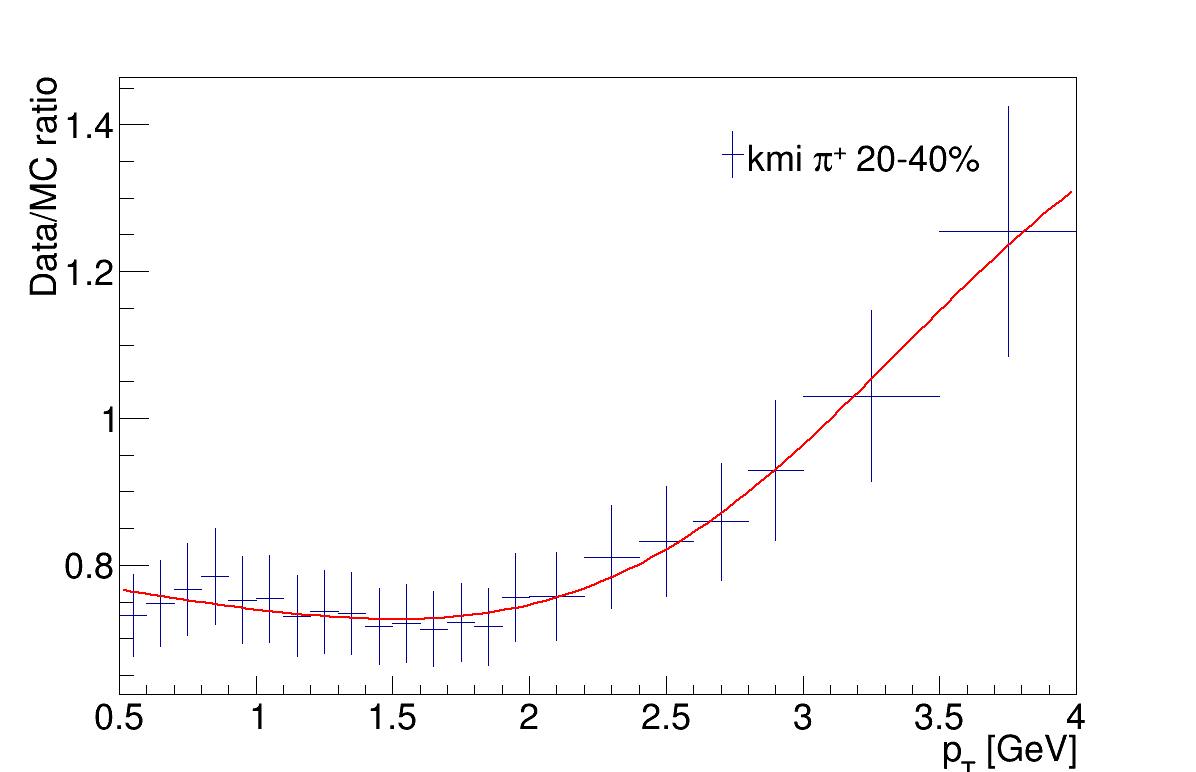
\includegraphics[width=0.24\linewidth]{detdeta/Figures/particle_reweighting_ratios/EPOS_kmi_2.png}
    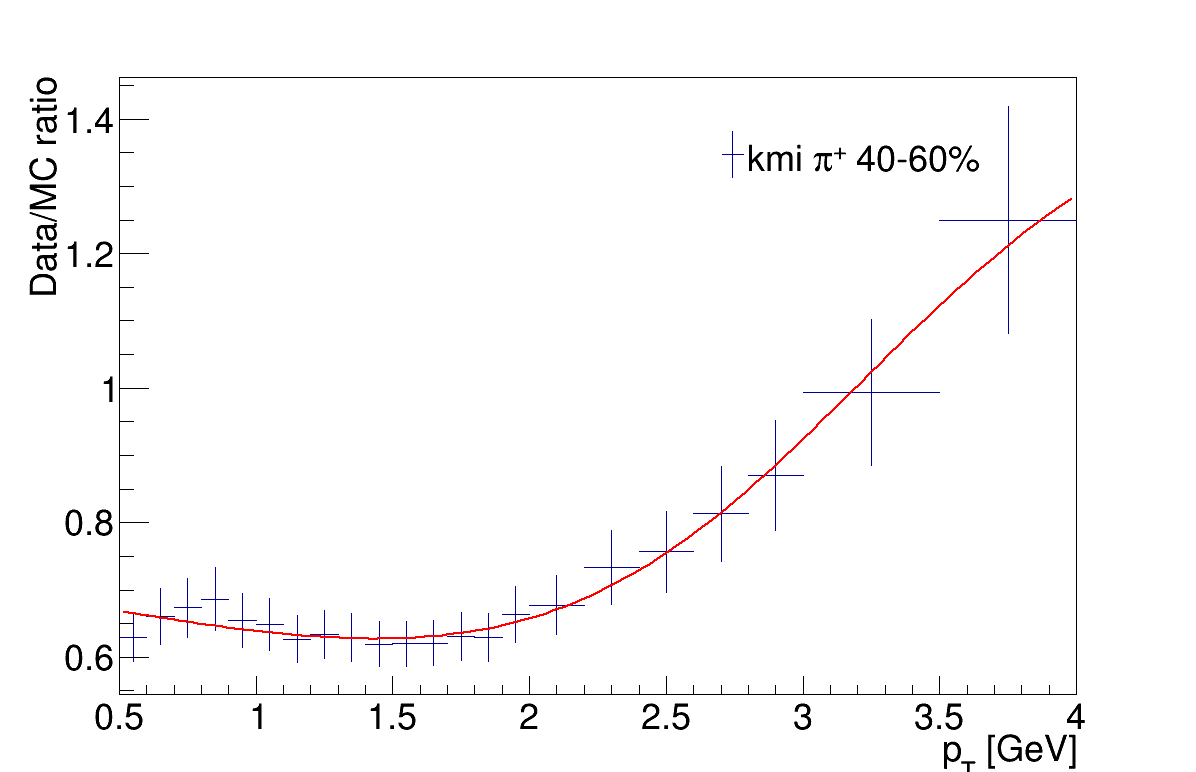
\includegraphics[width=0.24\linewidth]{detdeta/Figures/particle_reweighting_ratios/EPOS_kmi_3.png}
    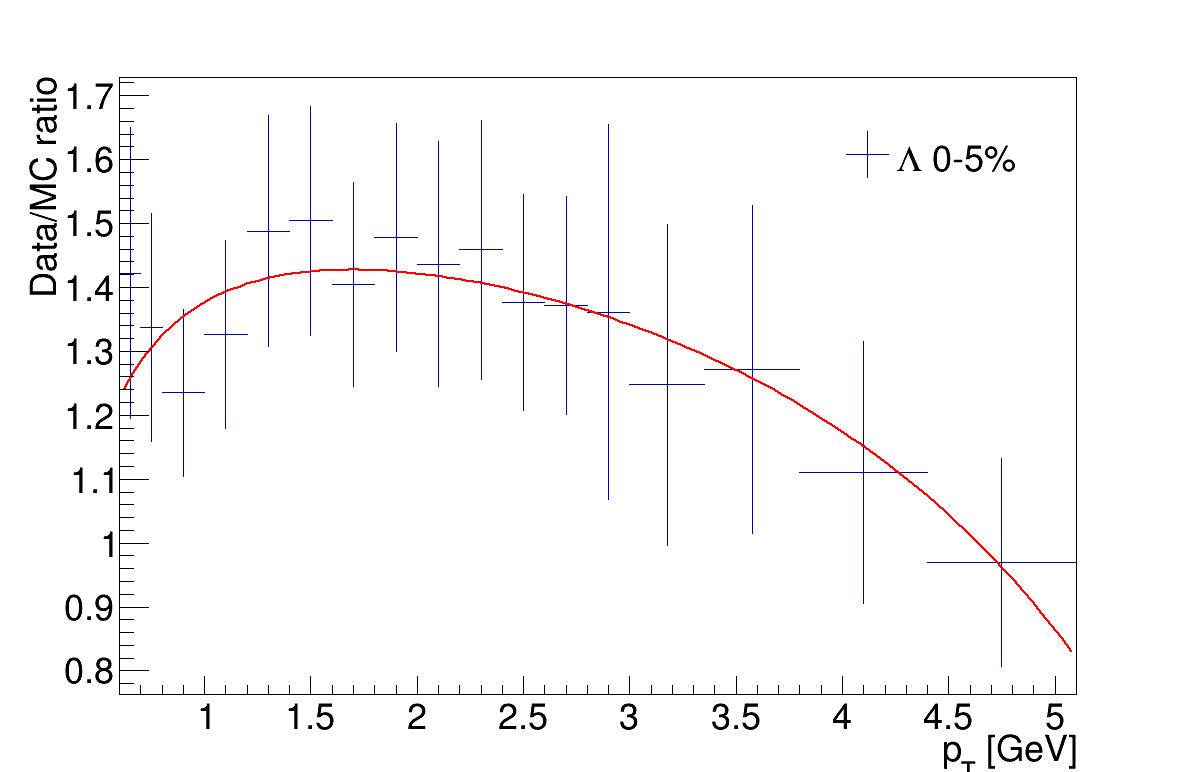
\includegraphics[width=0.24\linewidth]{detdeta/Figures/particle_reweighting_ratios/EPOS_lambda_0.png}
    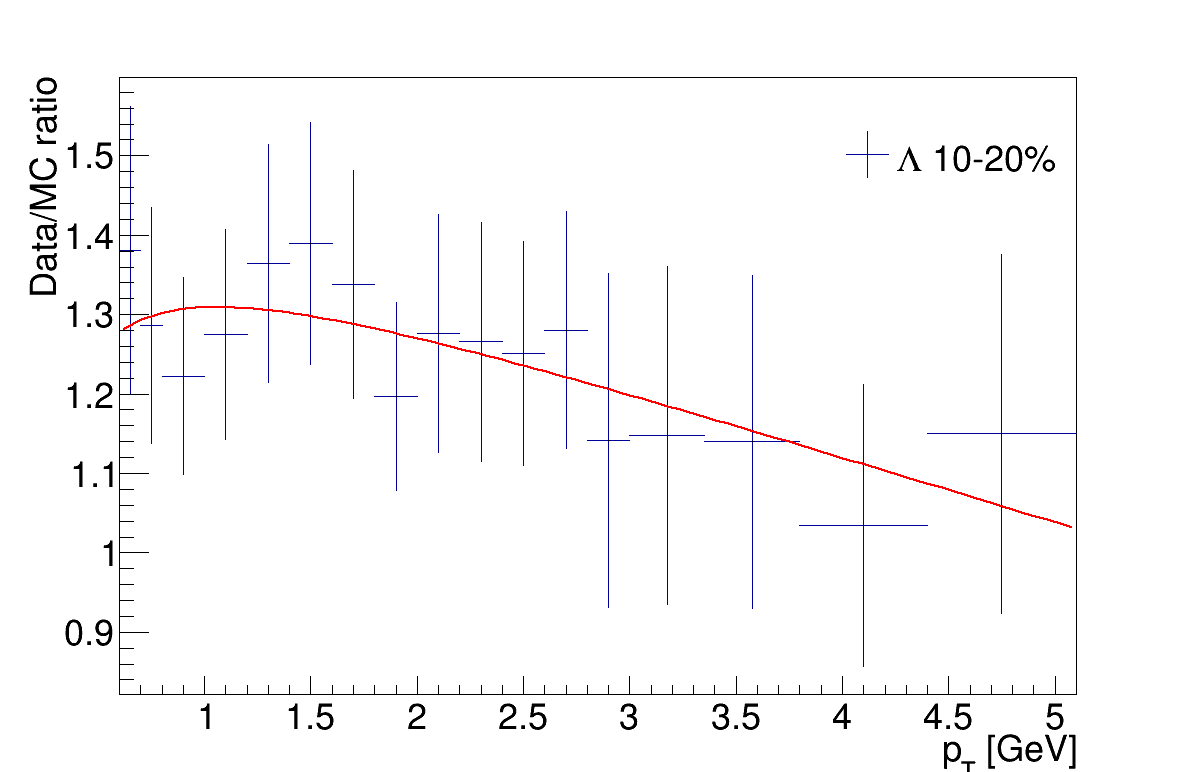
\includegraphics[width=0.24\linewidth]{detdeta/Figures/particle_reweighting_ratios/EPOS_lambda_1.png}
    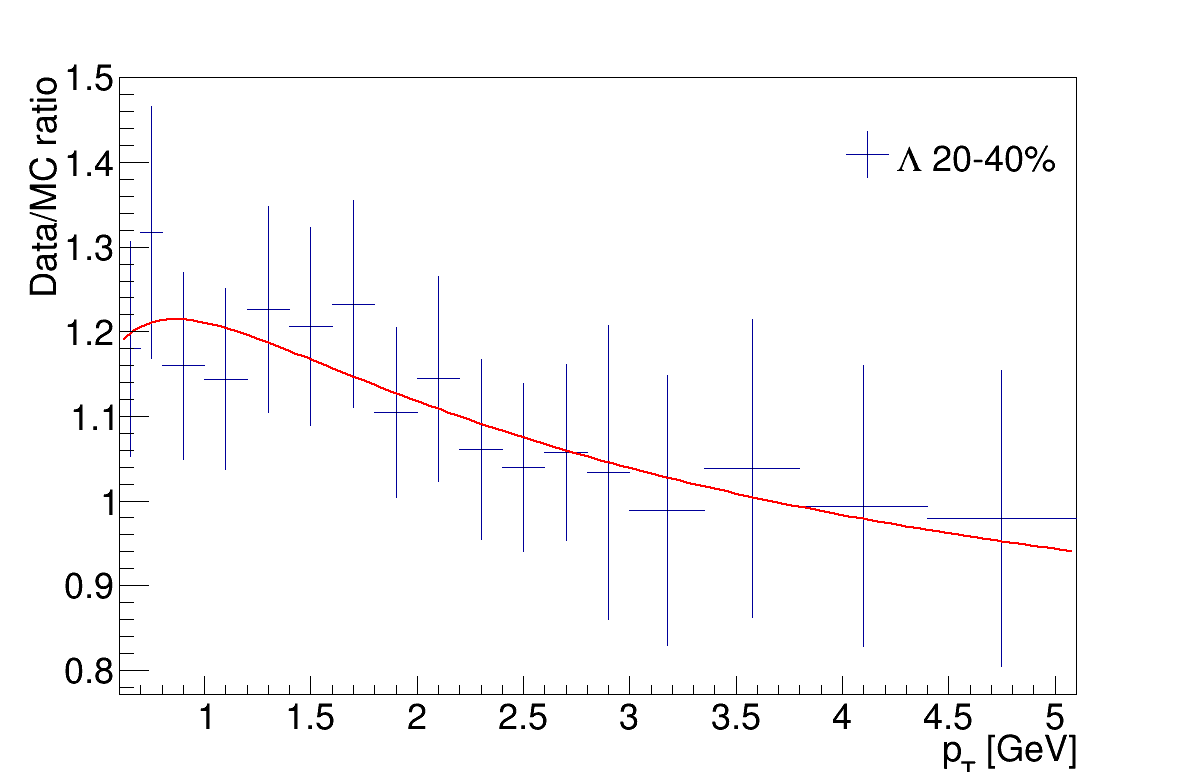
\includegraphics[width=0.24\linewidth]{detdeta/Figures/particle_reweighting_ratios/EPOS_lambda_2.png}
    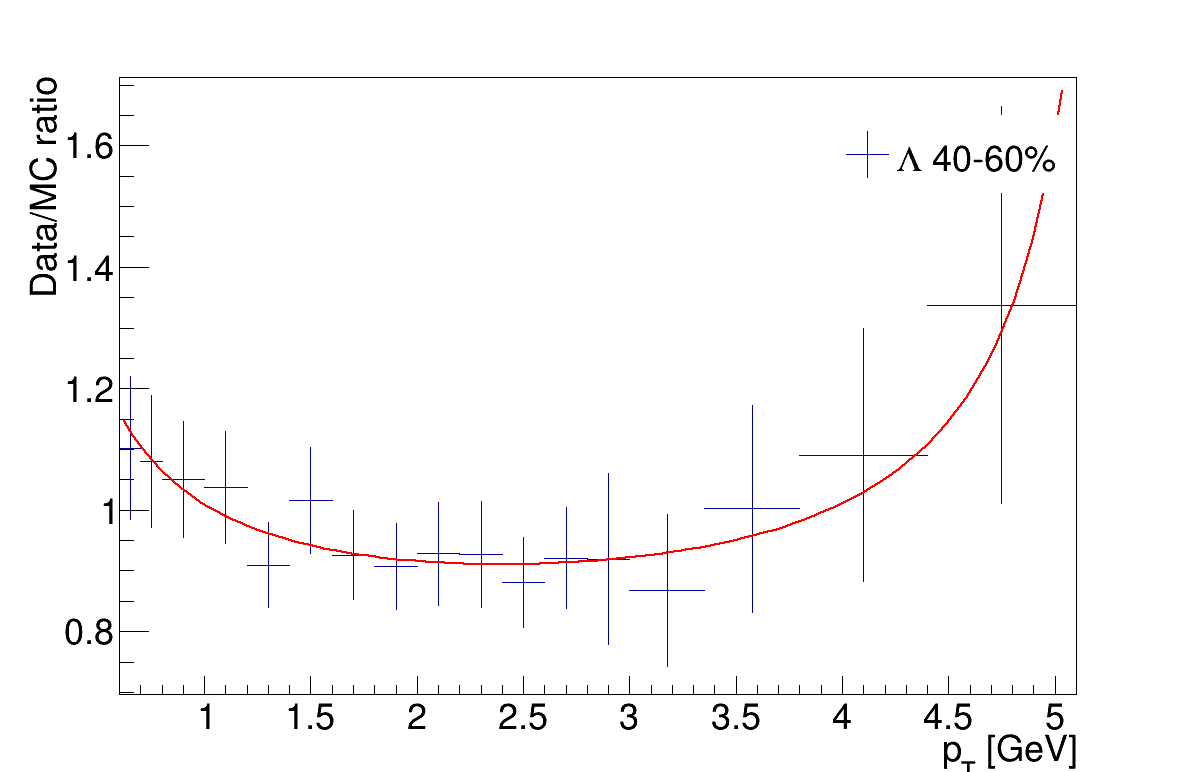
\includegraphics[width=0.24\linewidth]{detdeta/Figures/particle_reweighting_ratios/EPOS_lambda_3.png}
    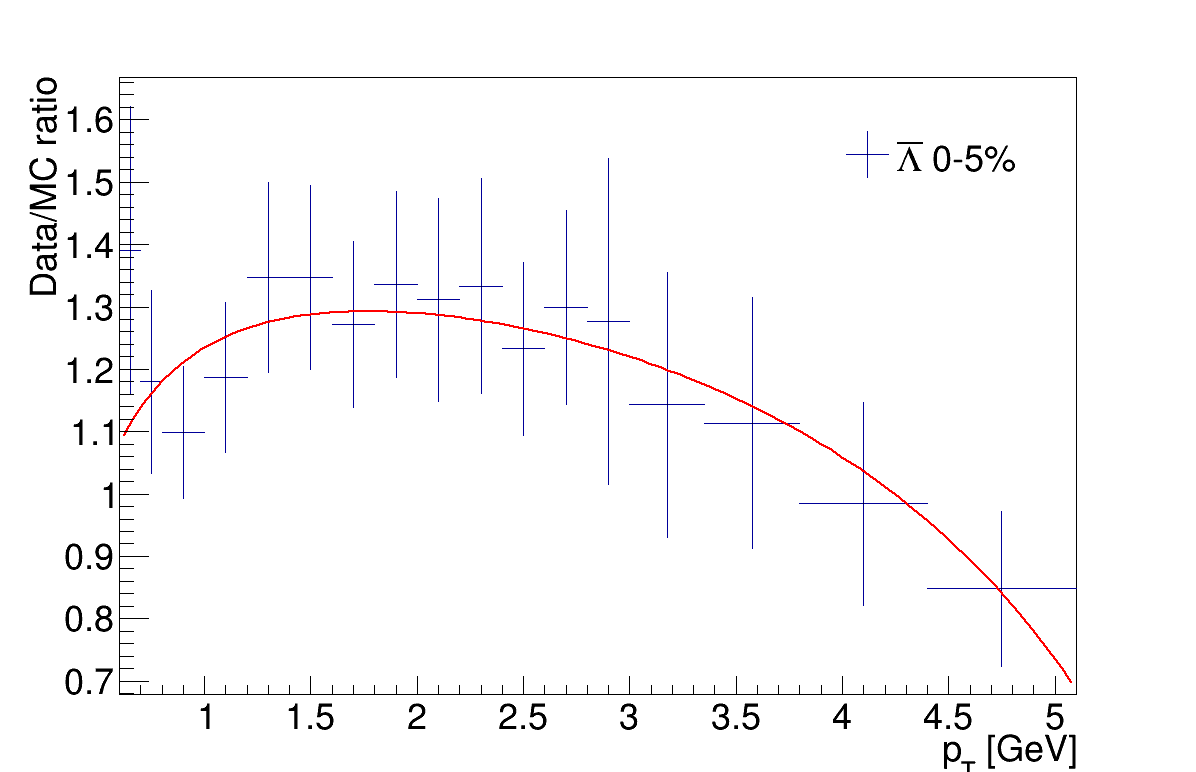
\includegraphics[width=0.24\linewidth]{detdeta/Figures/particle_reweighting_ratios/EPOS_lambda_bar_0.png}
    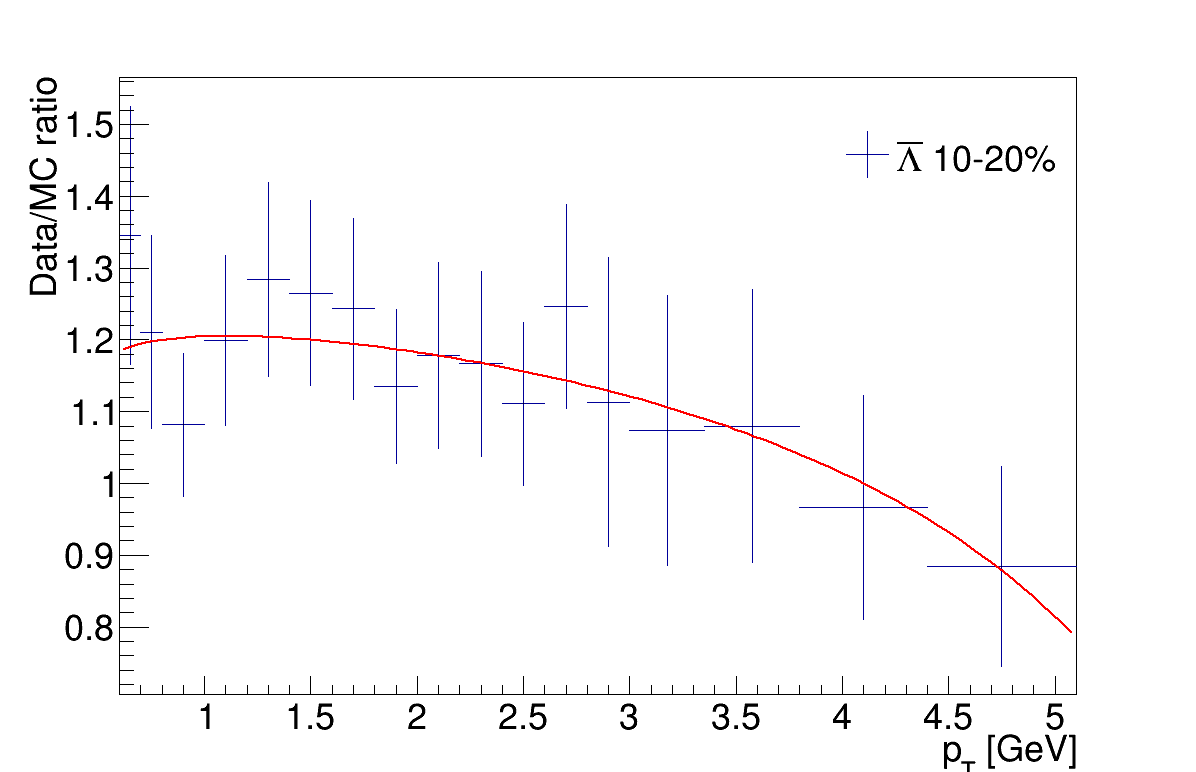
\includegraphics[width=0.24\linewidth]{detdeta/Figures/particle_reweighting_ratios/EPOS_lambda_bar_1.png}
    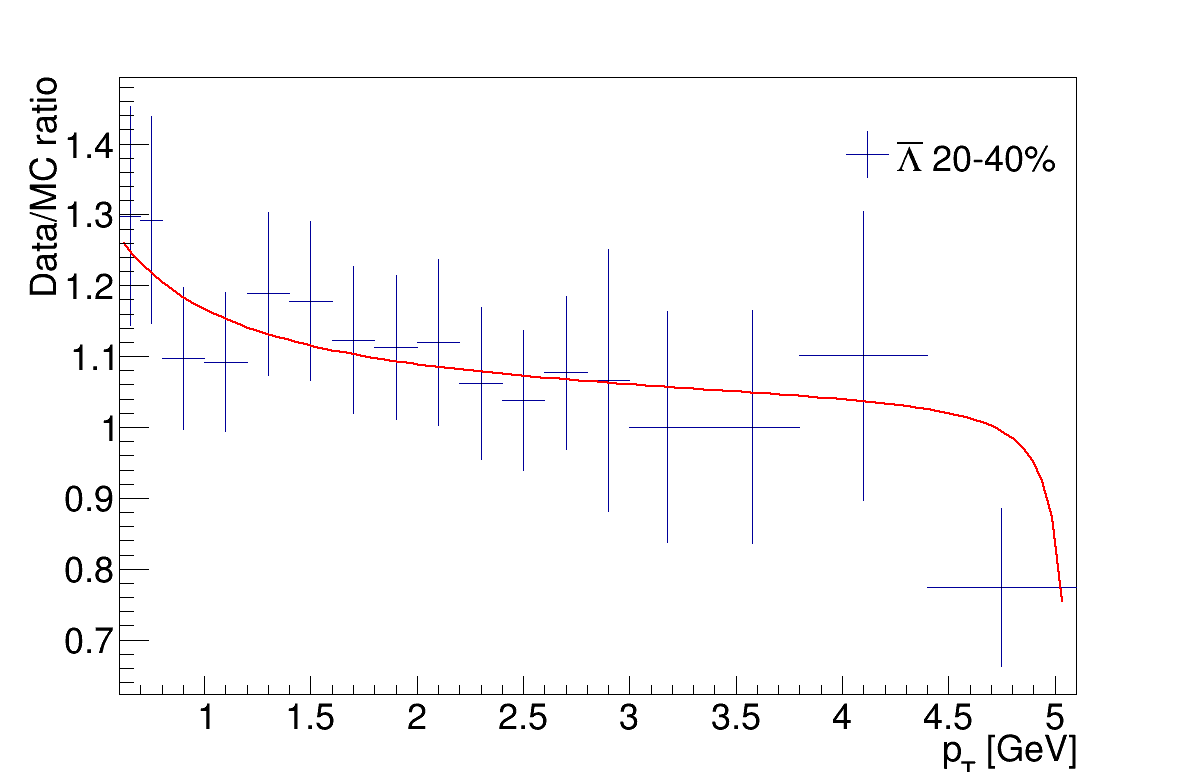
\includegraphics[width=0.24\linewidth]{detdeta/Figures/particle_reweighting_ratios/EPOS_lambda_bar_2.png}
    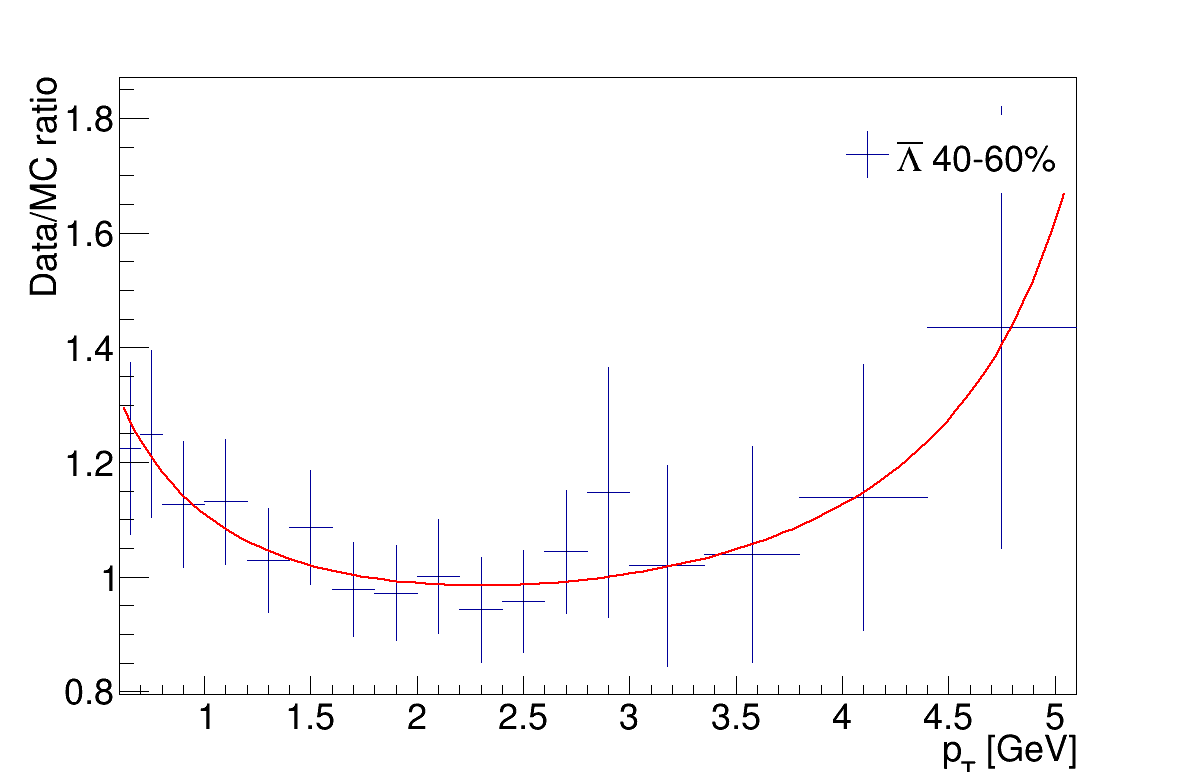
\includegraphics[width=0.24\linewidth]{detdeta/Figures/particle_reweighting_ratios/EPOS_lambda_bar_3.png}
    \caption{All data to MC ratios used in nominal EPOS reweighting method for protons, anti-protons, kaons, pions and lambda particles.}
    \label{fig:epos_data_mc_particle_ratios}
\end{figure}

\begin{figure}
    \centering
    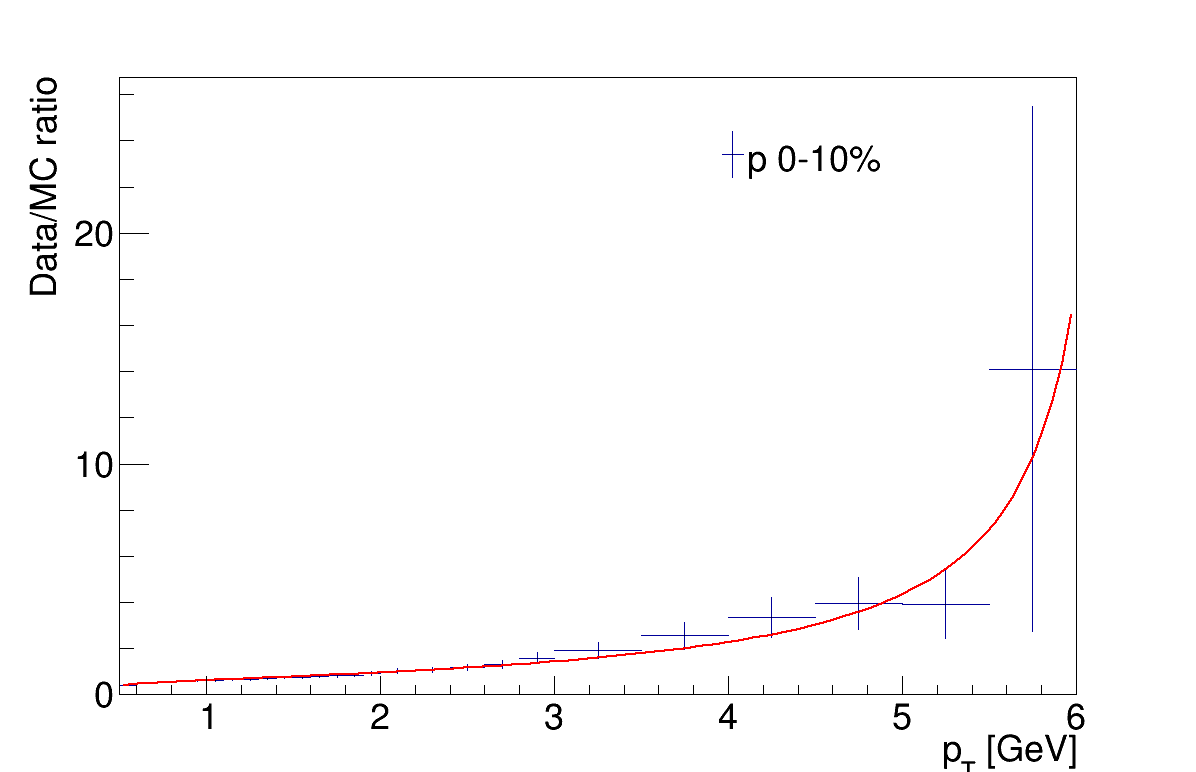
\includegraphics[width=0.24\linewidth]{detdeta/Figures/particle_reweighting_ratios/AMPT_p_0.png}
    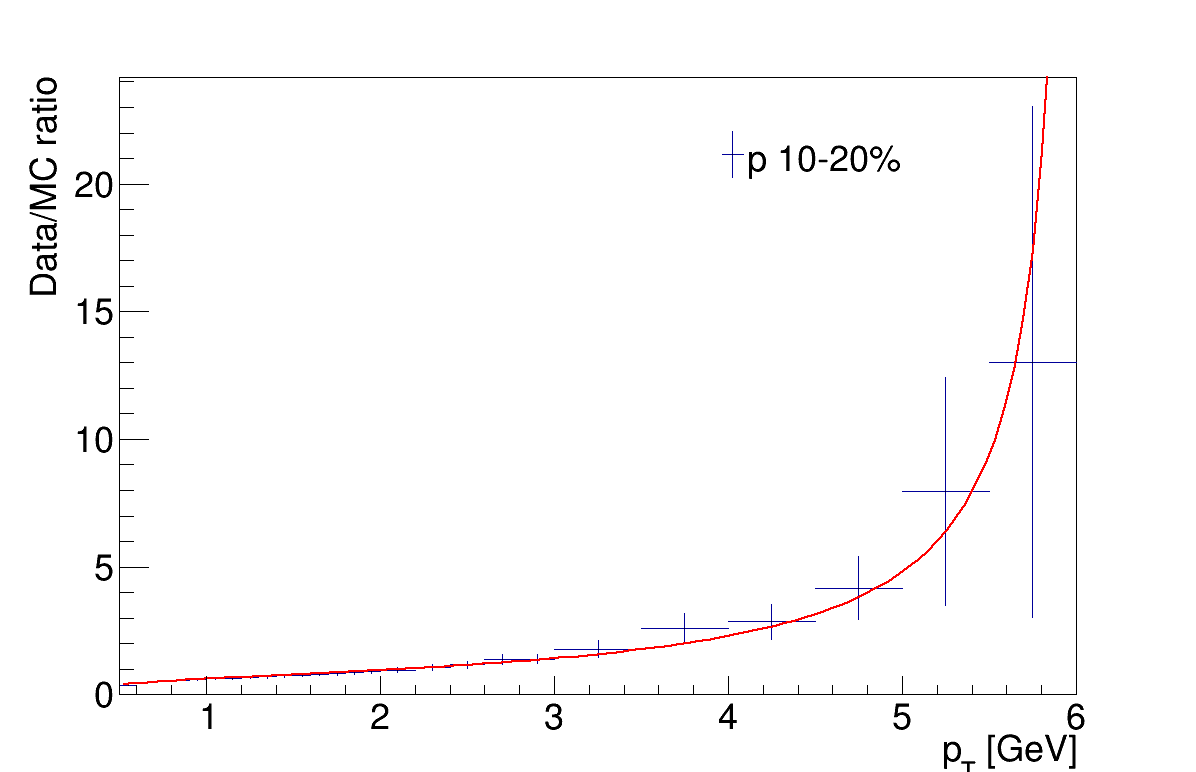
\includegraphics[width=0.24\linewidth]{detdeta/Figures/particle_reweighting_ratios/AMPT_p_1.png}
    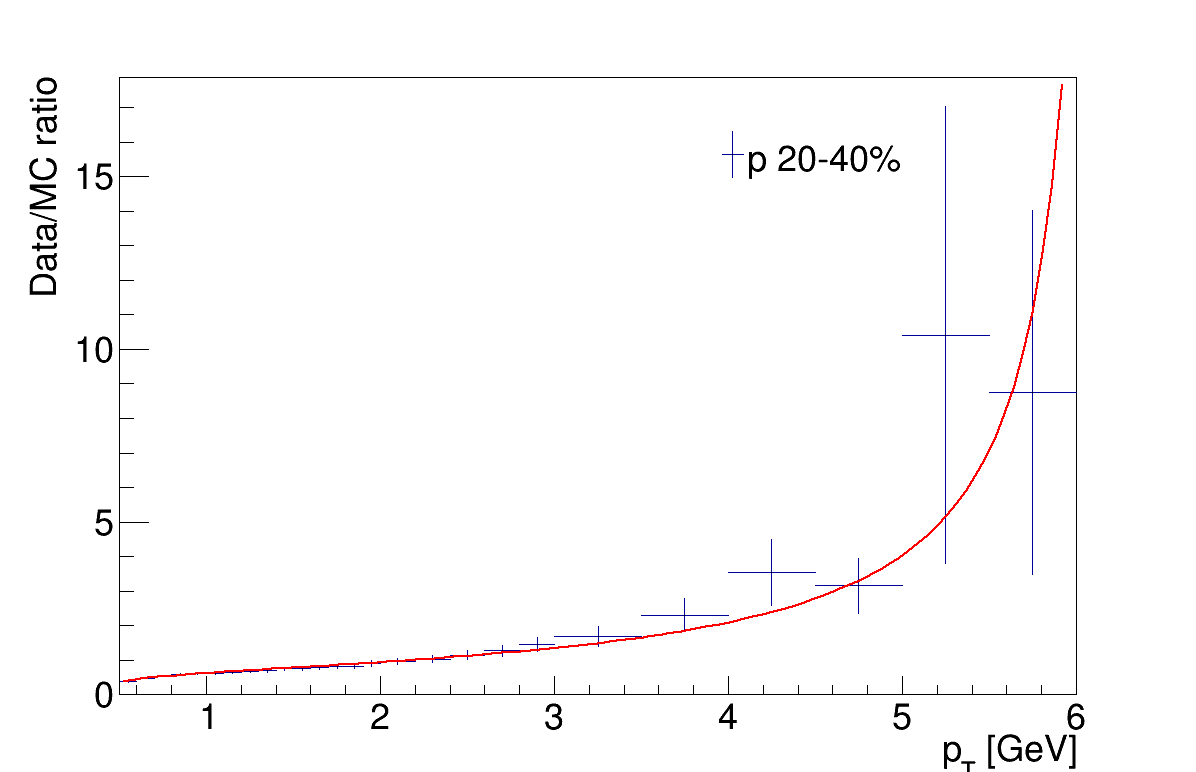
\includegraphics[width=0.24\linewidth]{detdeta/Figures/particle_reweighting_ratios/AMPT_p_2.png}
    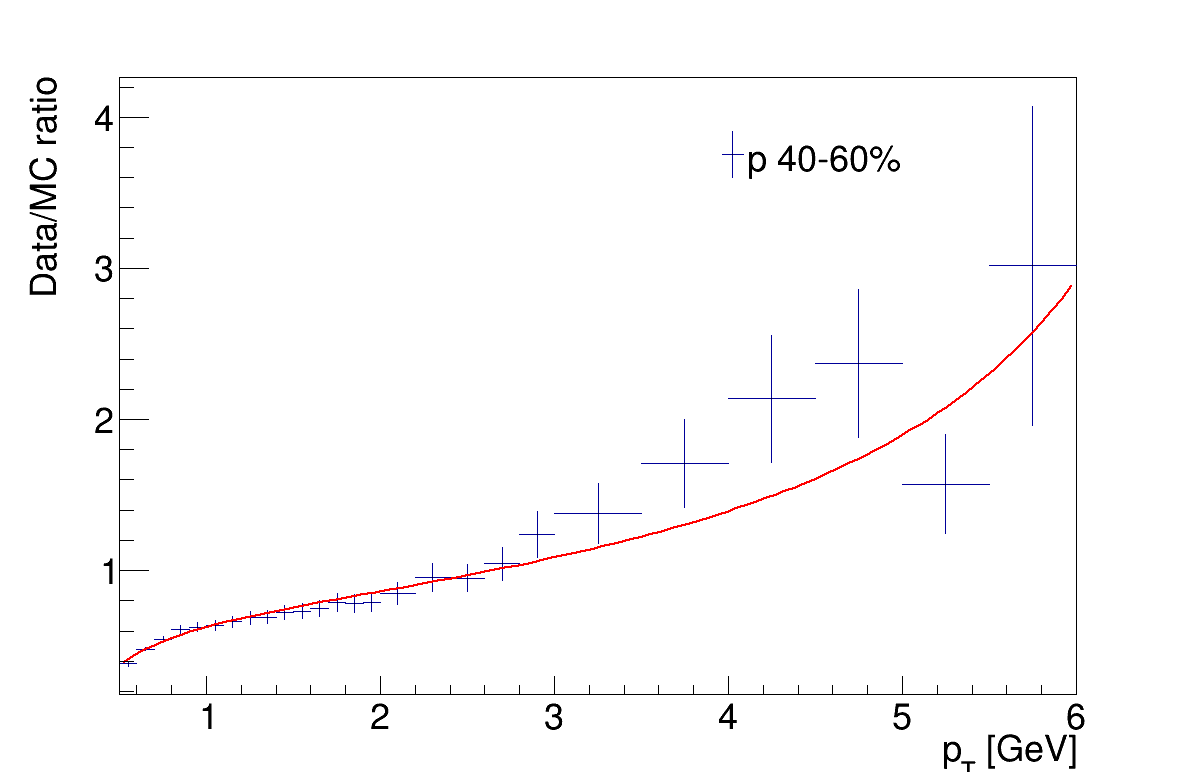
\includegraphics[width=0.24\linewidth]{detdeta/Figures/particle_reweighting_ratios/AMPT_p_3.png}
    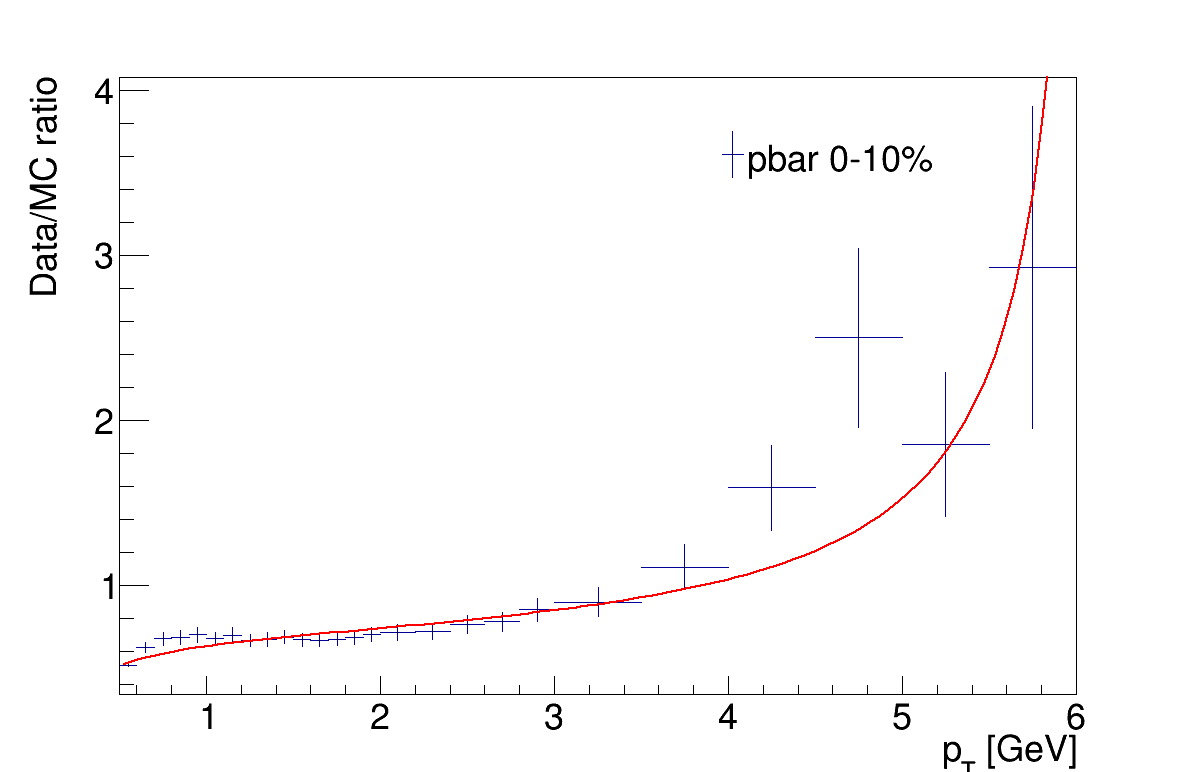
\includegraphics[width=0.24\linewidth]{detdeta/Figures/particle_reweighting_ratios/AMPT_pbar_0.png}
    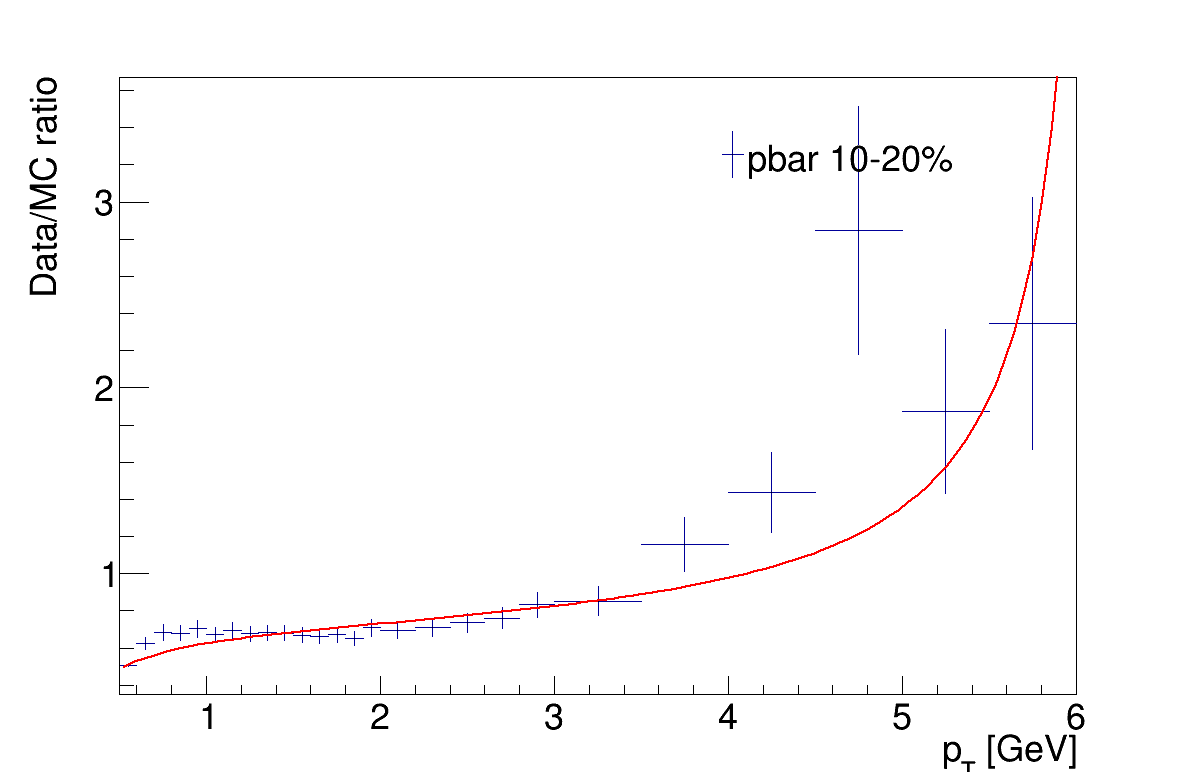
\includegraphics[width=0.24\linewidth]{detdeta/Figures/particle_reweighting_ratios/AMPT_pbar_1.png}
    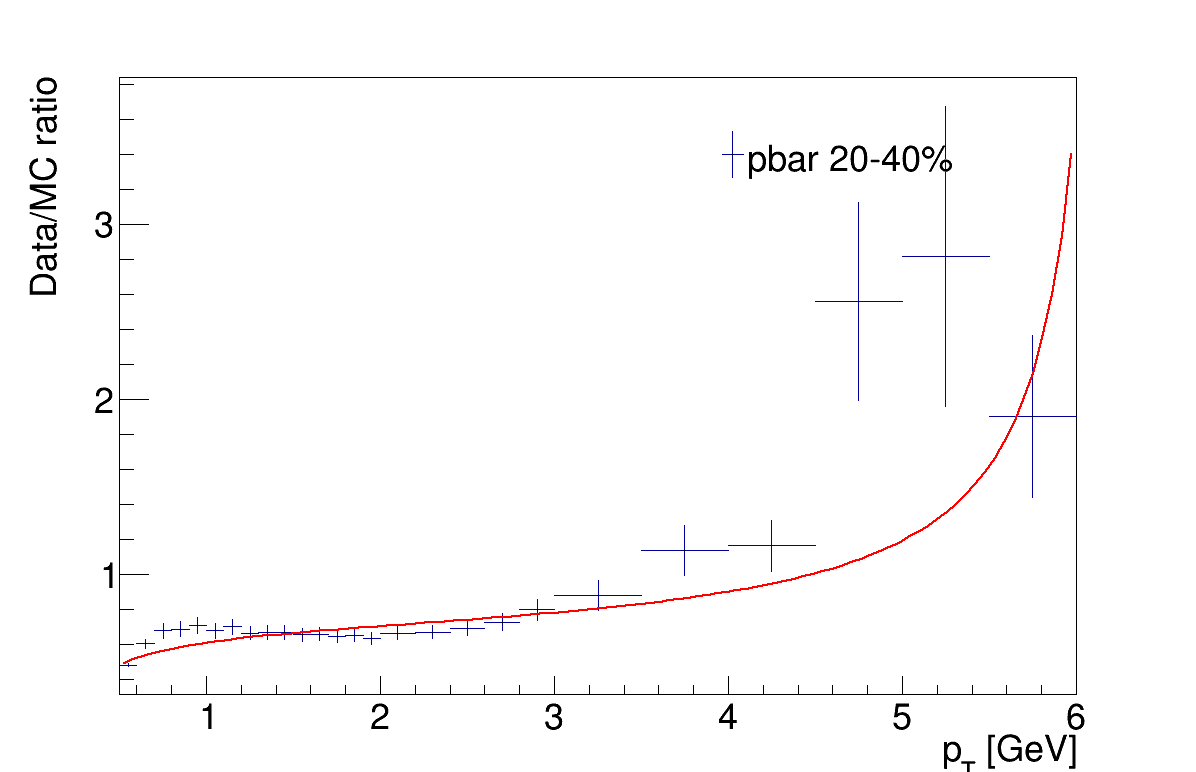
\includegraphics[width=0.24\linewidth]{detdeta/Figures/particle_reweighting_ratios/AMPT_pbar_2.png}
    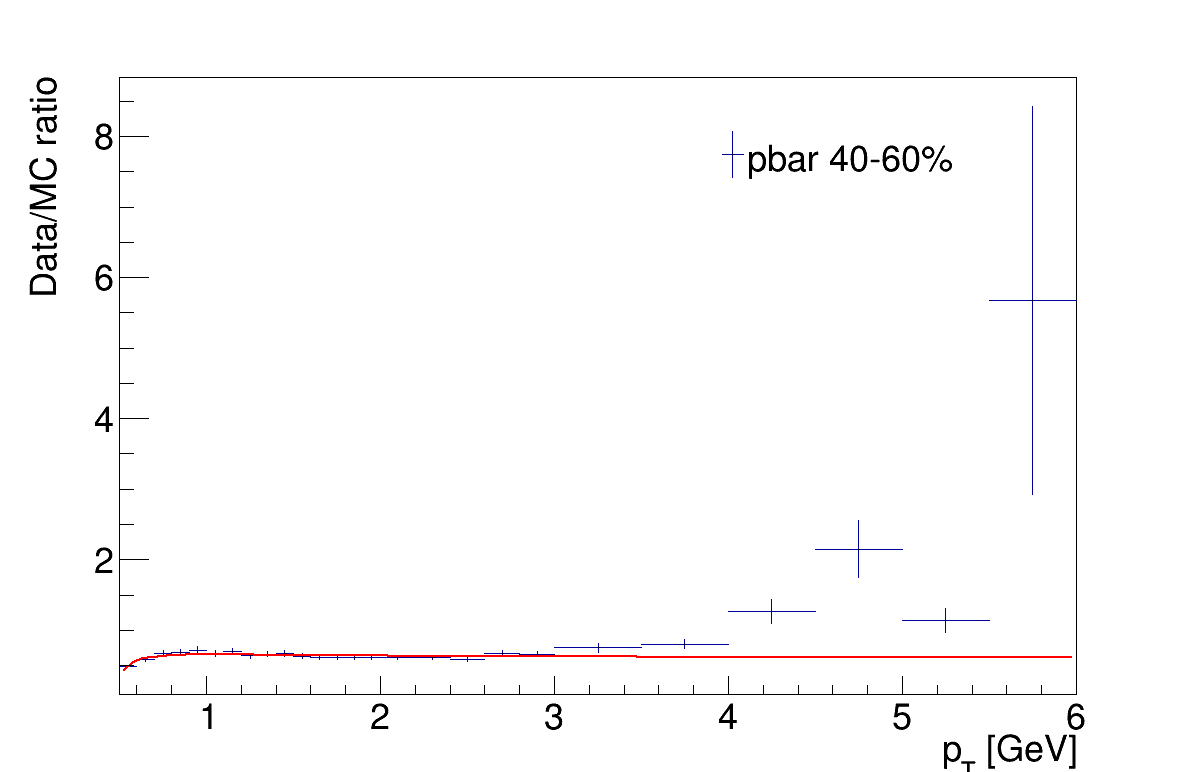
\includegraphics[width=0.24\linewidth]{detdeta/Figures/particle_reweighting_ratios/AMPT_pbar_3.png}
    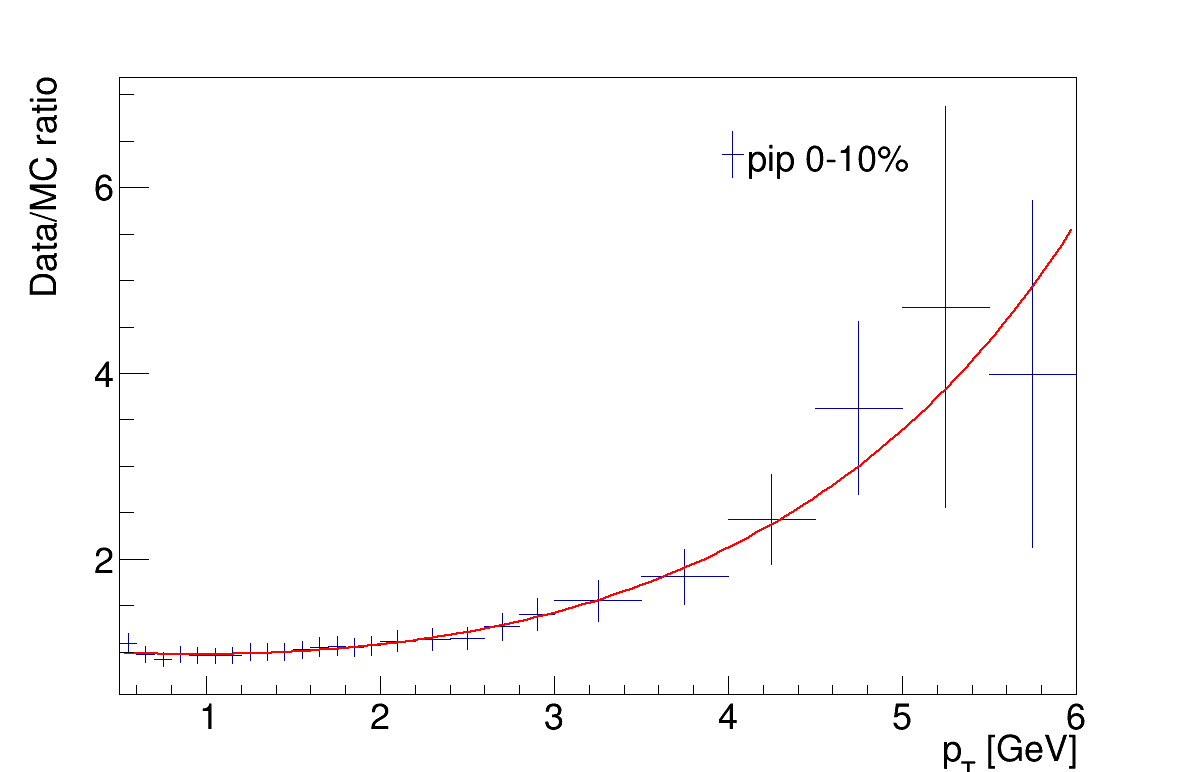
\includegraphics[width=0.24\linewidth]{detdeta/Figures/particle_reweighting_ratios/AMPT_pip_0.png}
    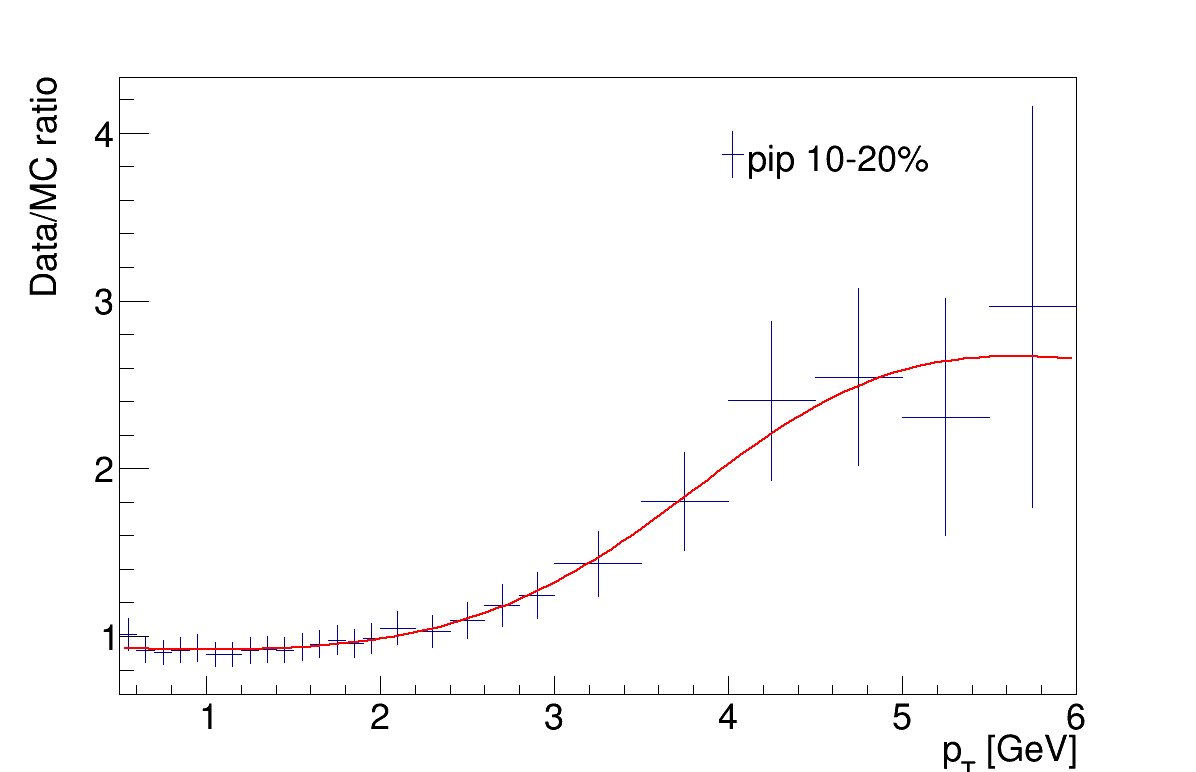
\includegraphics[width=0.24\linewidth]{detdeta/Figures/particle_reweighting_ratios/AMPT_pip_1.png}
    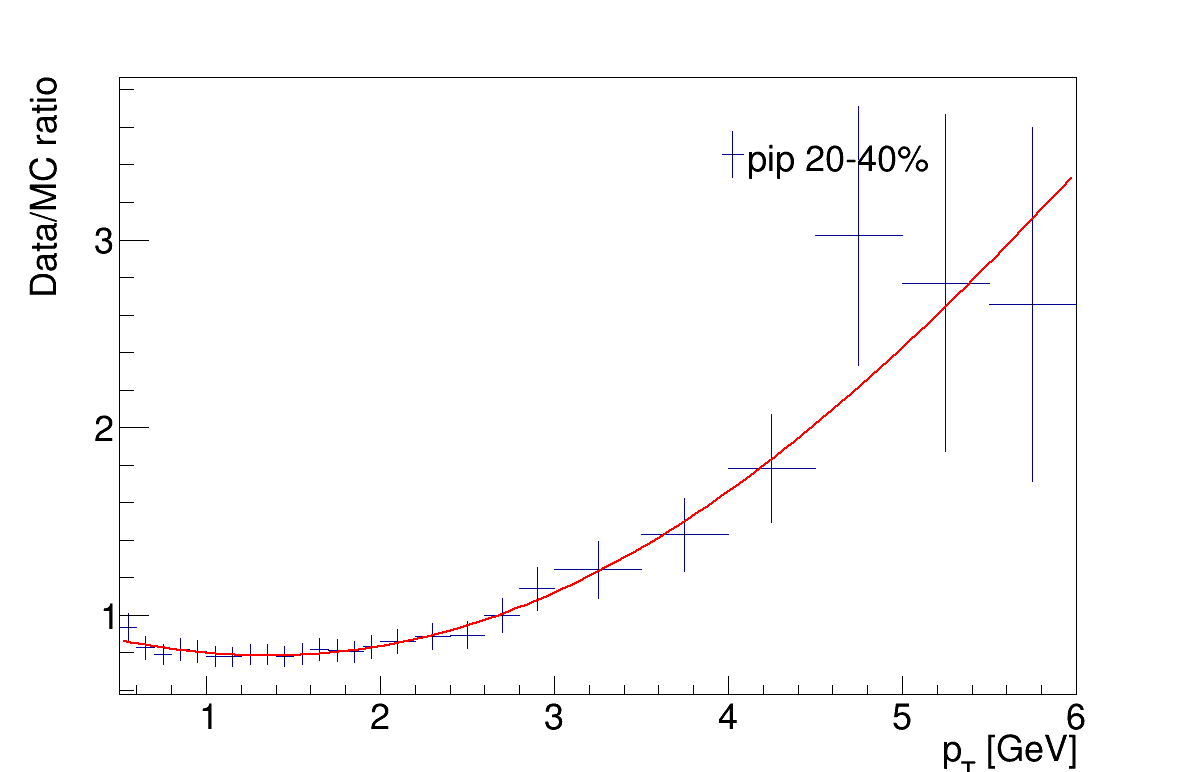
\includegraphics[width=0.24\linewidth]{detdeta/Figures/particle_reweighting_ratios/AMPT_pip_2.png}
    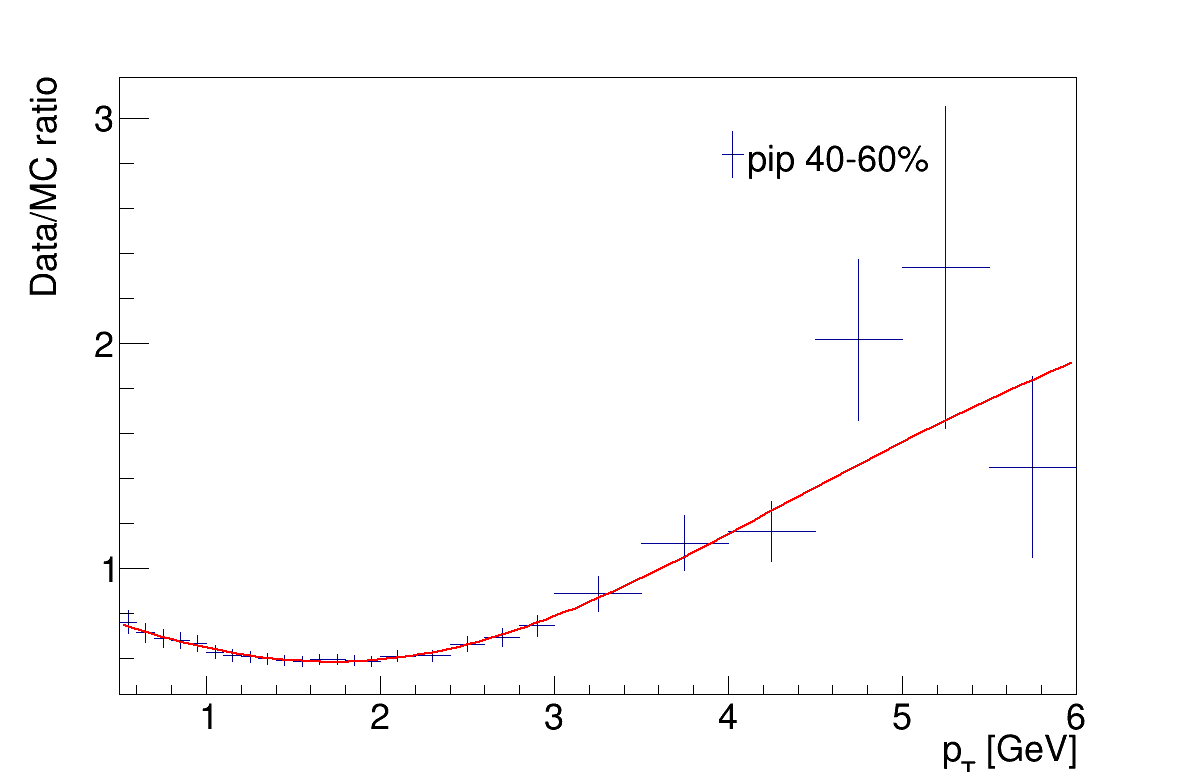
\includegraphics[width=0.24\linewidth]{detdeta/Figures/particle_reweighting_ratios/AMPT_pip_3.png}
    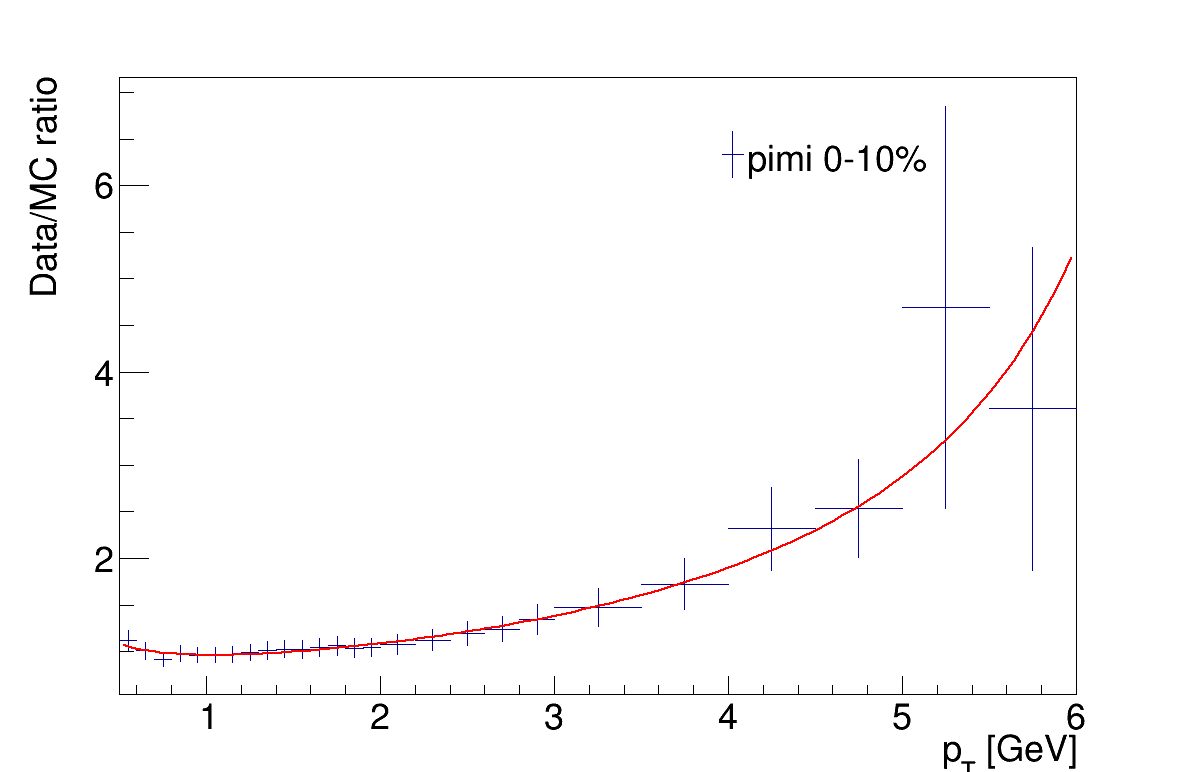
\includegraphics[width=0.24\linewidth]{detdeta/Figures/particle_reweighting_ratios/AMPT_pimi_0.png}
    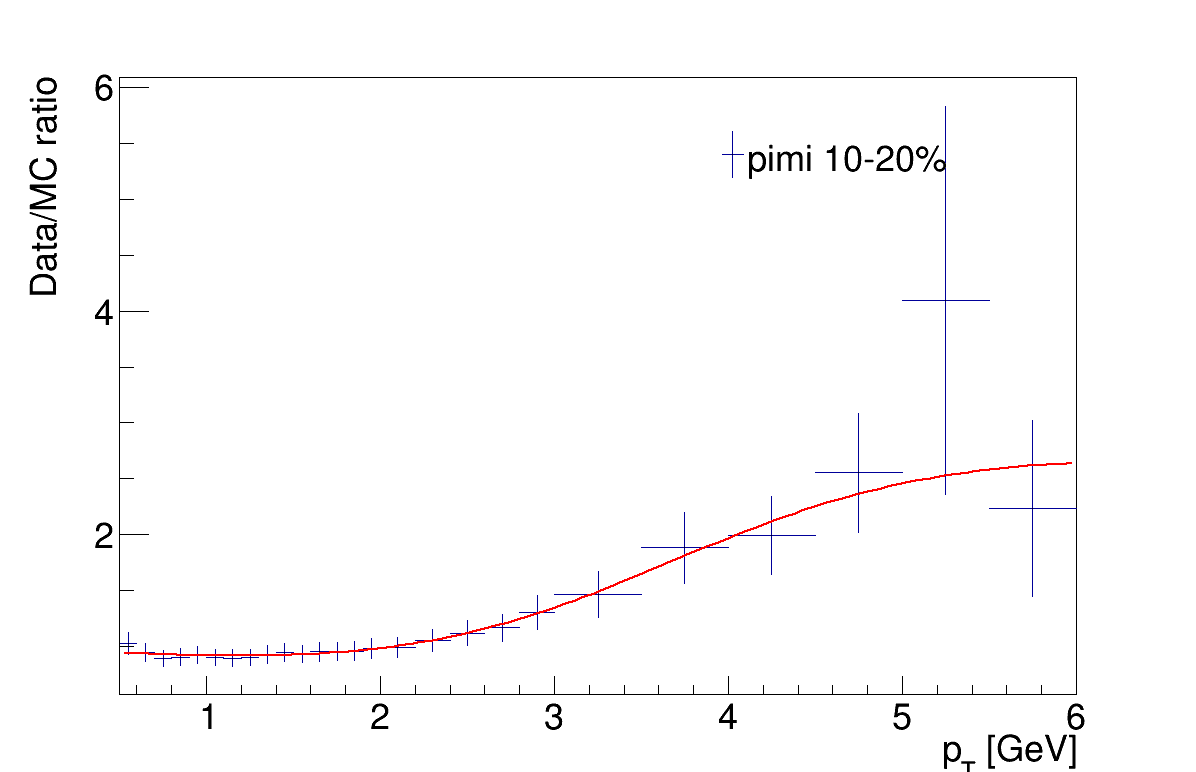
\includegraphics[width=0.24\linewidth]{detdeta/Figures/particle_reweighting_ratios/AMPT_pimi_1.png}
    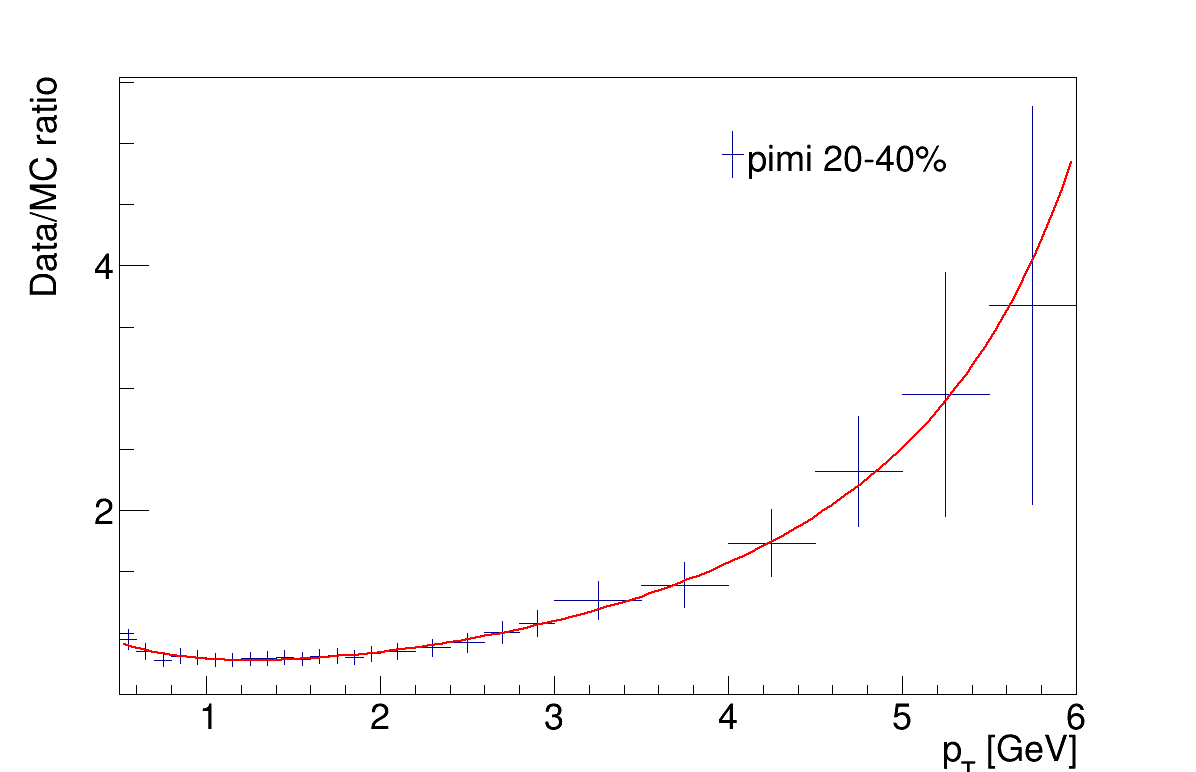
\includegraphics[width=0.24\linewidth]{detdeta/Figures/particle_reweighting_ratios/AMPT_pimi_2.png}
    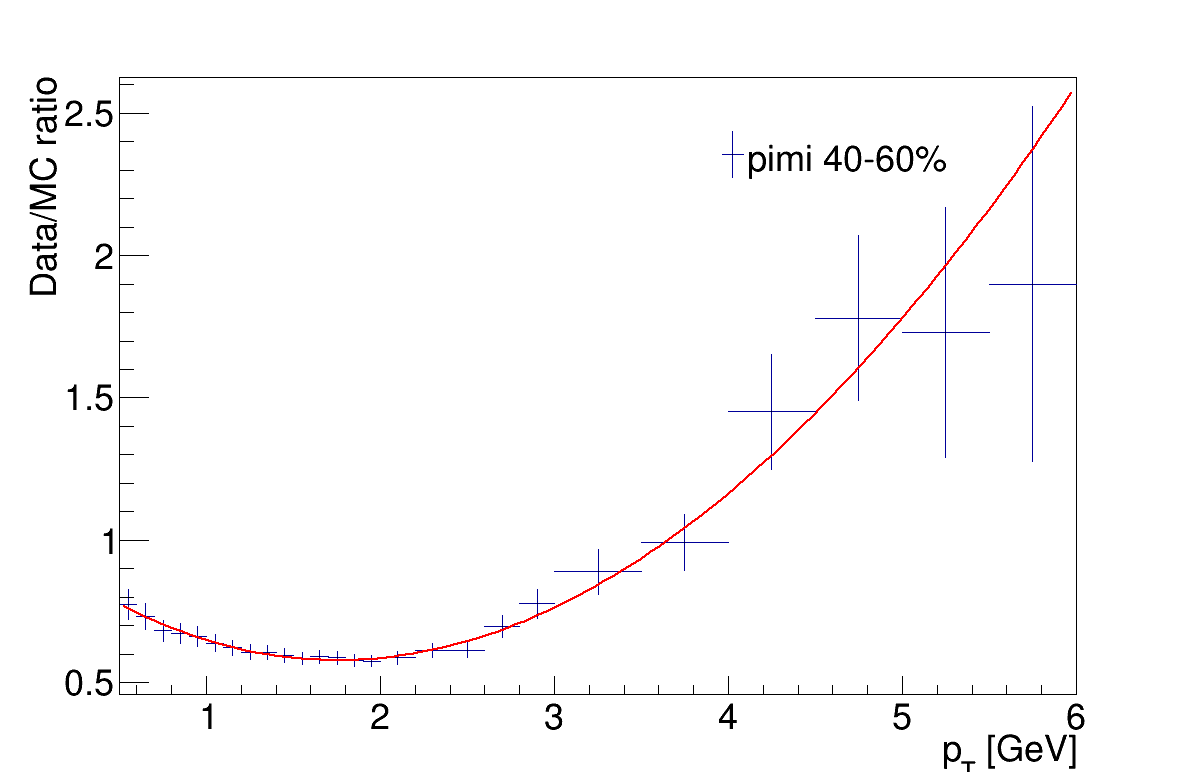
\includegraphics[width=0.24\linewidth]{detdeta/Figures/particle_reweighting_ratios/AMPT_pimi_3.png}
    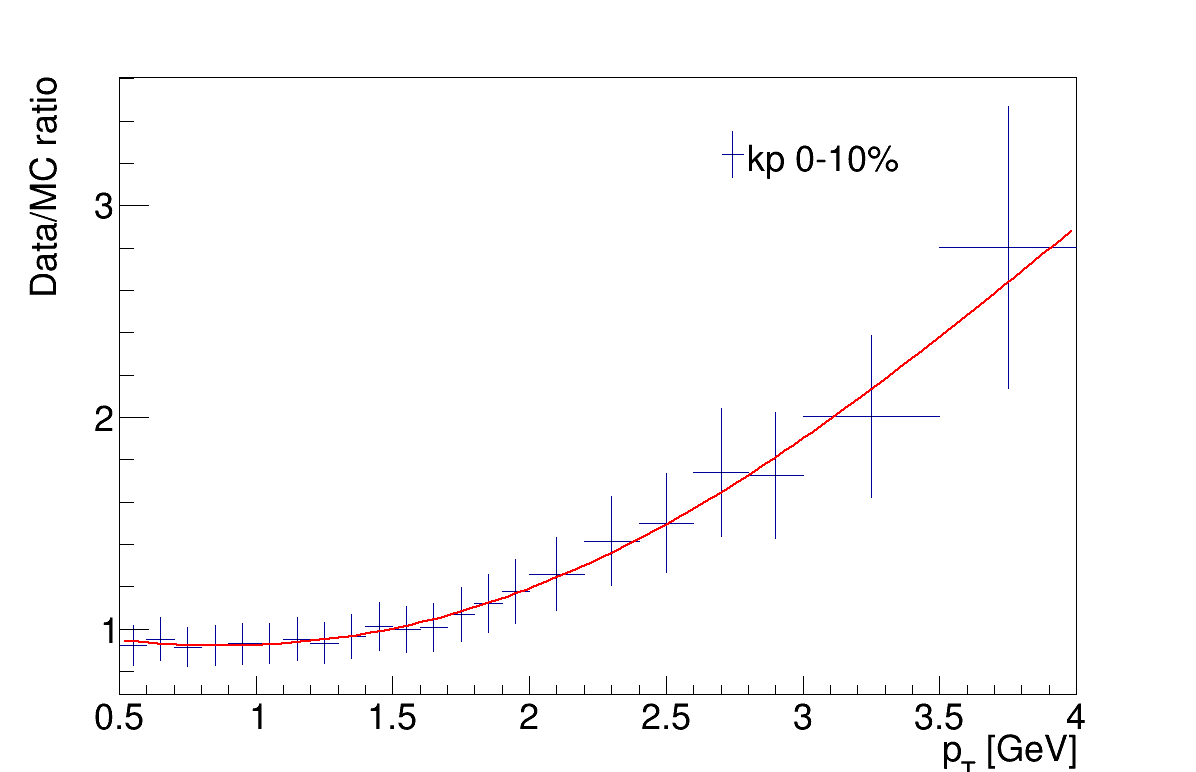
\includegraphics[width=0.24\linewidth]{detdeta/Figures/particle_reweighting_ratios/AMPT_kp_0.png}
    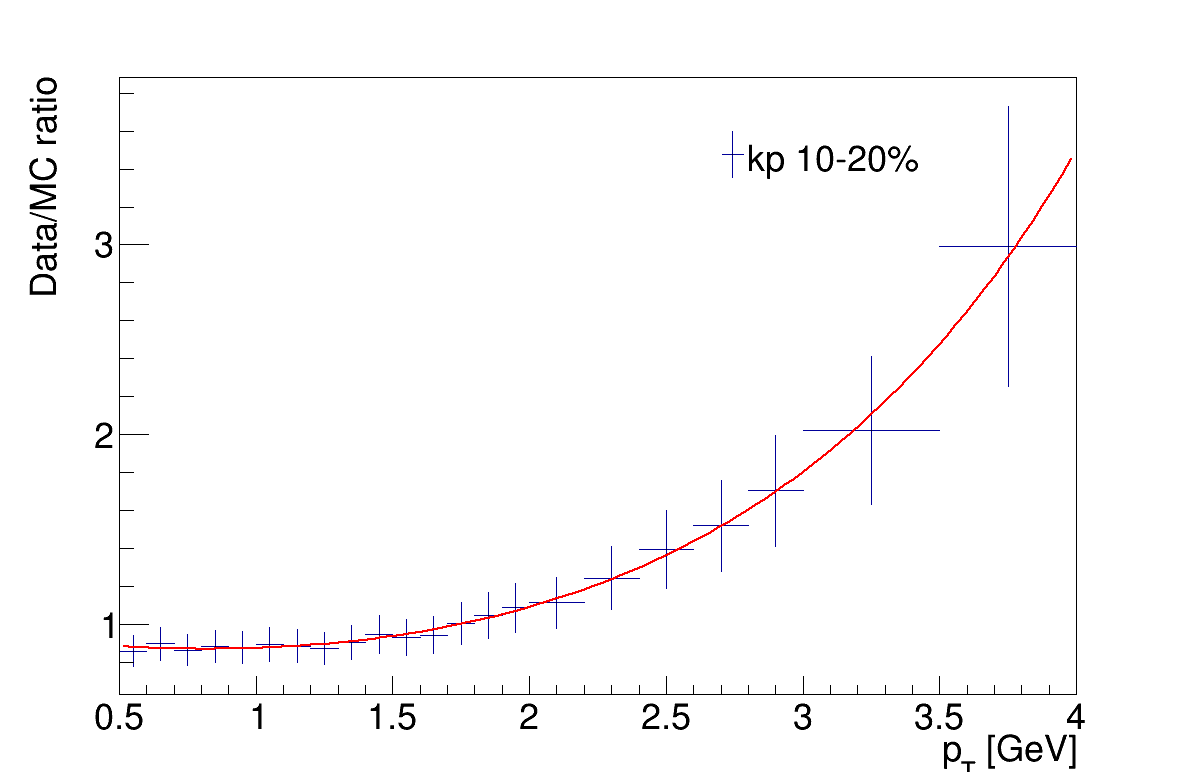
\includegraphics[width=0.24\linewidth]{detdeta/Figures/particle_reweighting_ratios/AMPT_kp_1.png}
    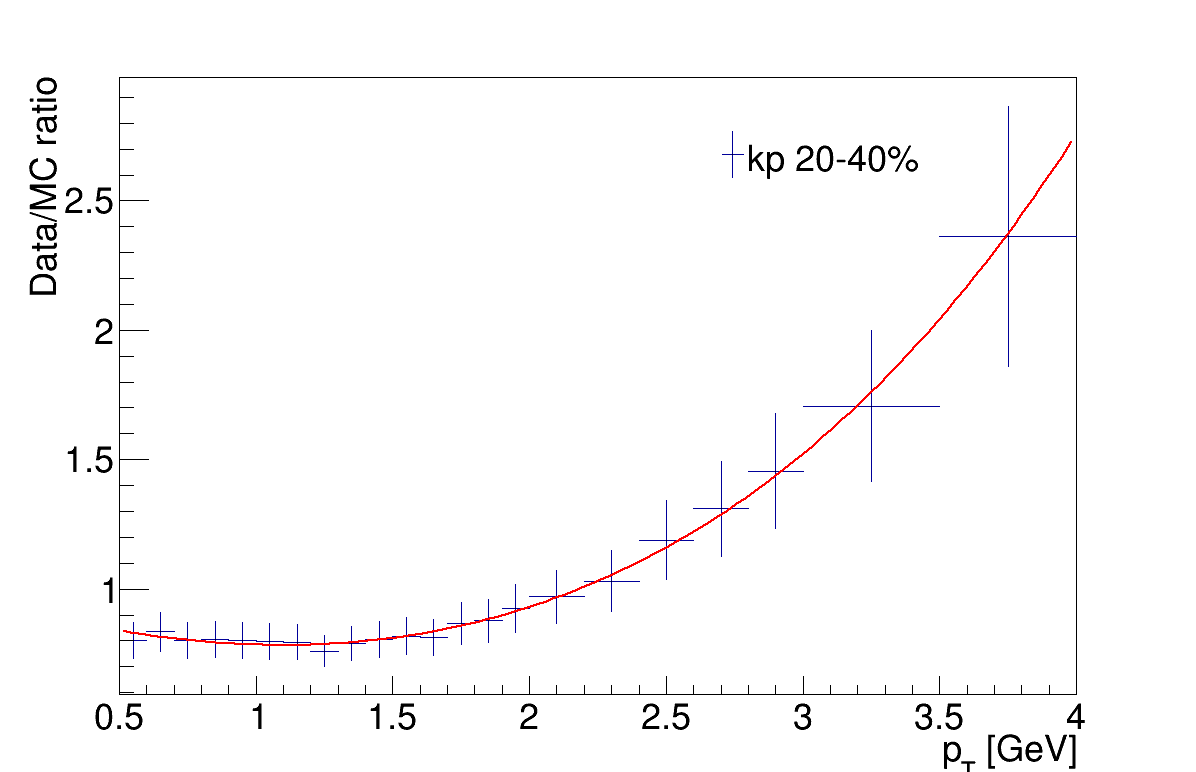
\includegraphics[width=0.24\linewidth]{detdeta/Figures/particle_reweighting_ratios/AMPT_kp_2.png}
    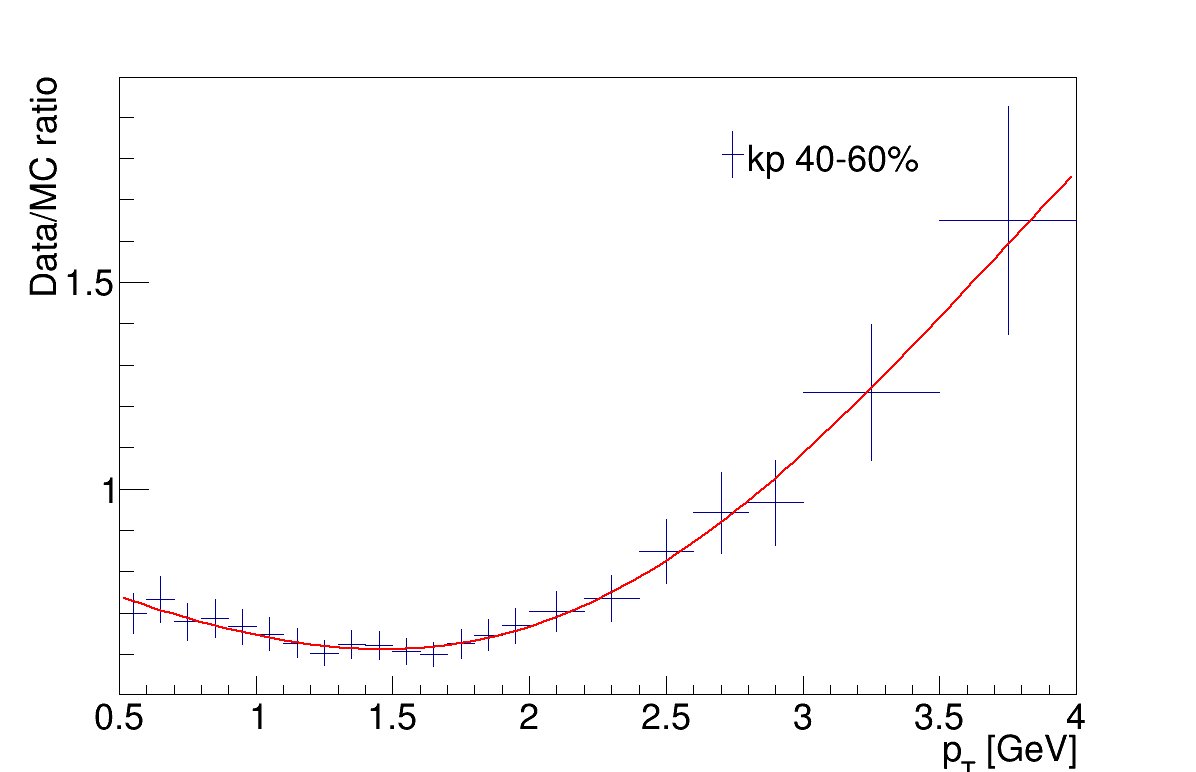
\includegraphics[width=0.24\linewidth]{detdeta/Figures/particle_reweighting_ratios/AMPT_kp_3.png}
    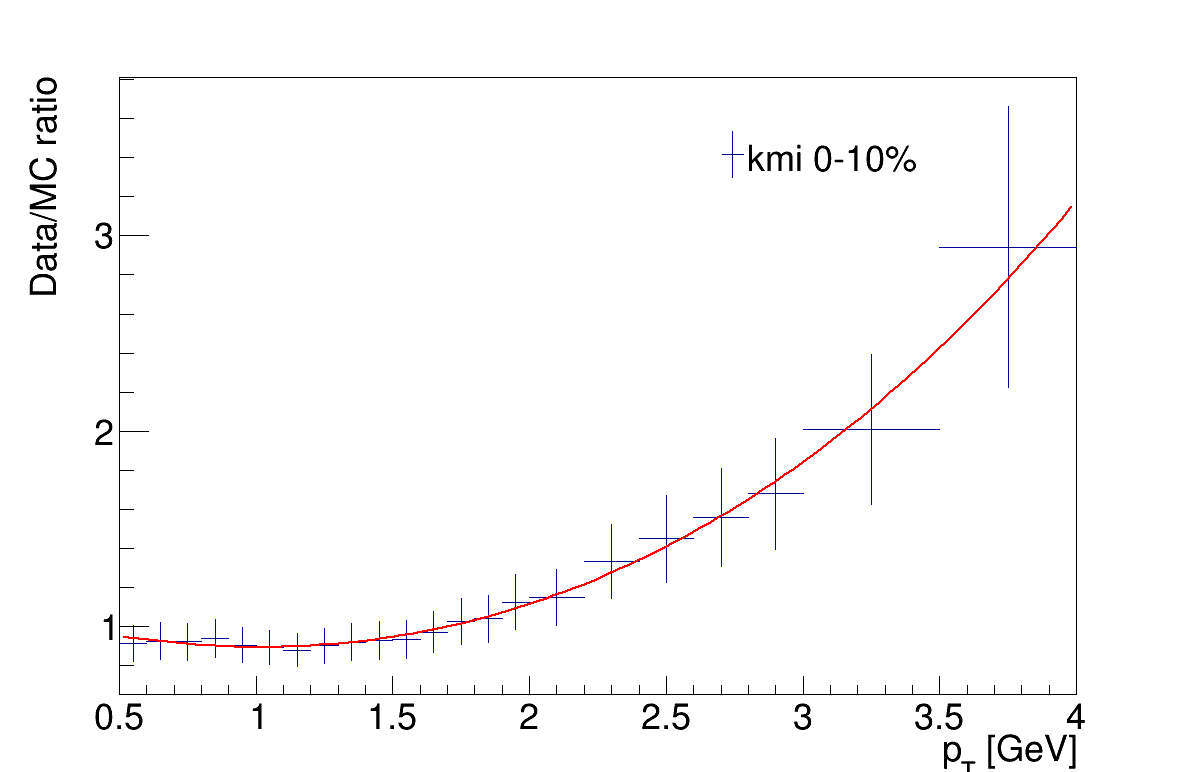
\includegraphics[width=0.24\linewidth]{detdeta/Figures/particle_reweighting_ratios/AMPT_kmi_0.png}
    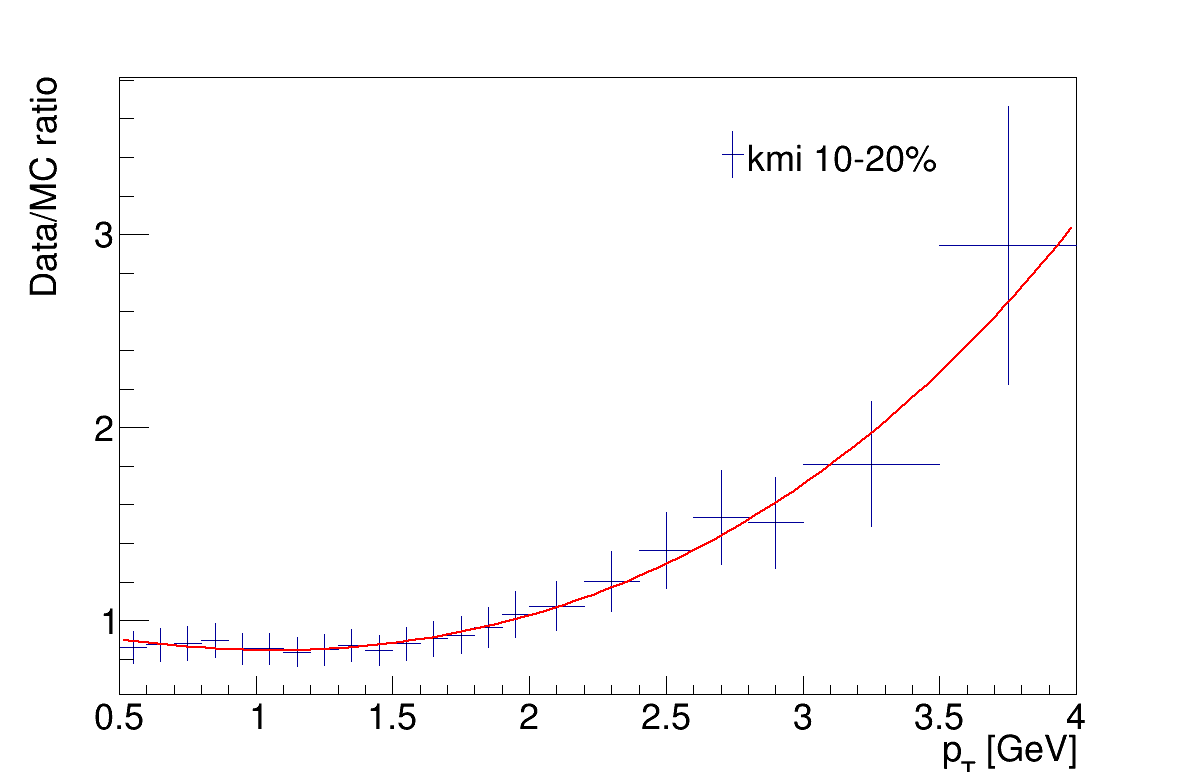
\includegraphics[width=0.24\linewidth]{detdeta/Figures/particle_reweighting_ratios/AMPT_kmi_1.png}
    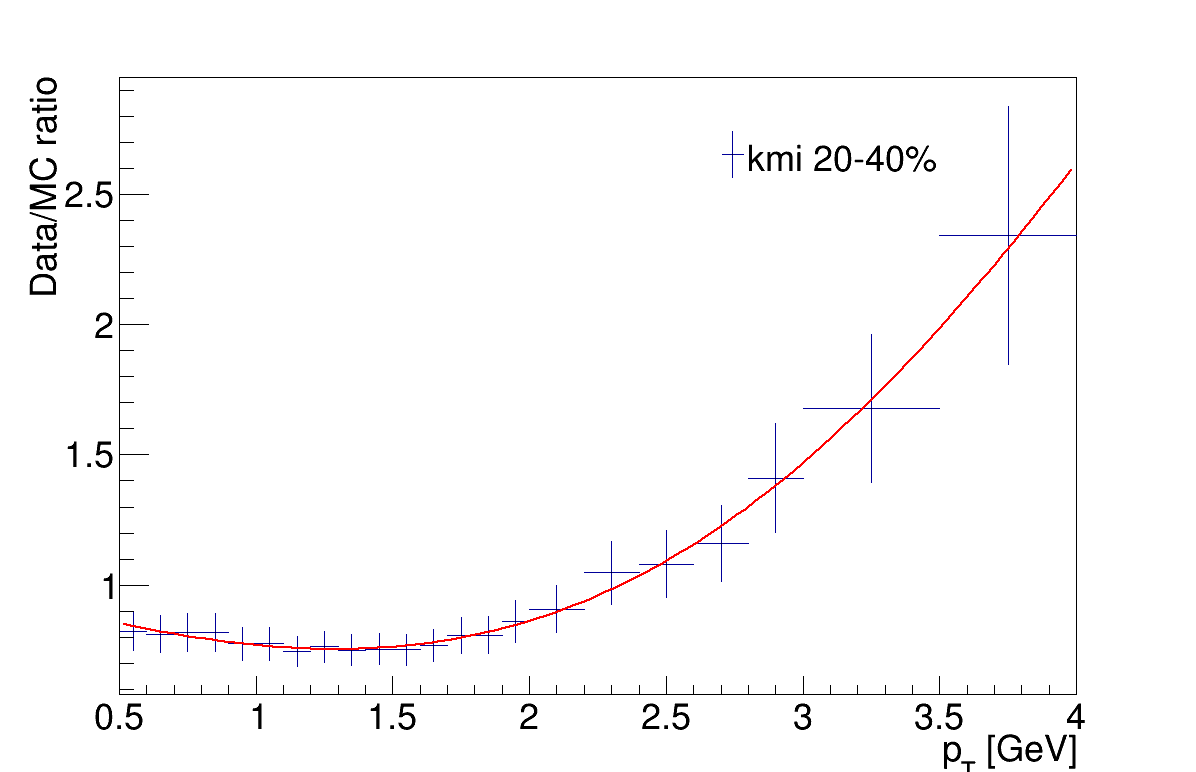
\includegraphics[width=0.24\linewidth]{detdeta/Figures/particle_reweighting_ratios/AMPT_kmi_2.png}
    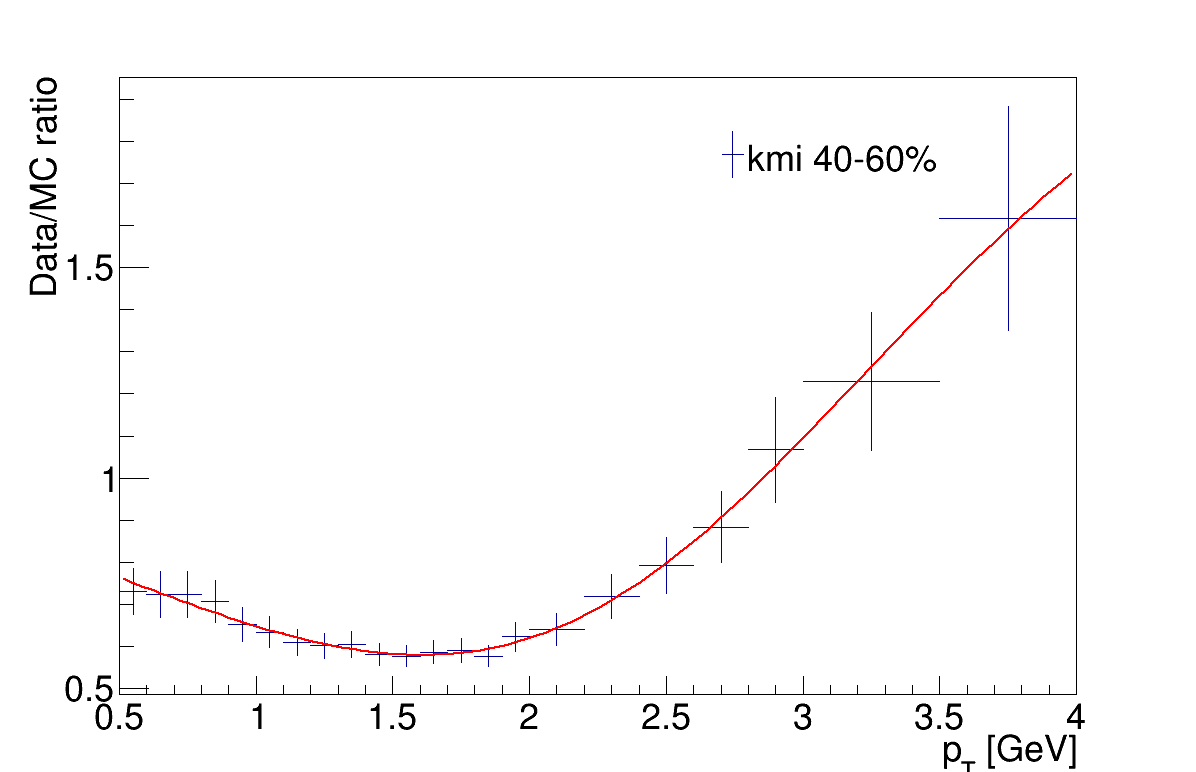
\includegraphics[width=0.24\linewidth]{detdeta/Figures/particle_reweighting_ratios/AMPT_kmi_3.png}
    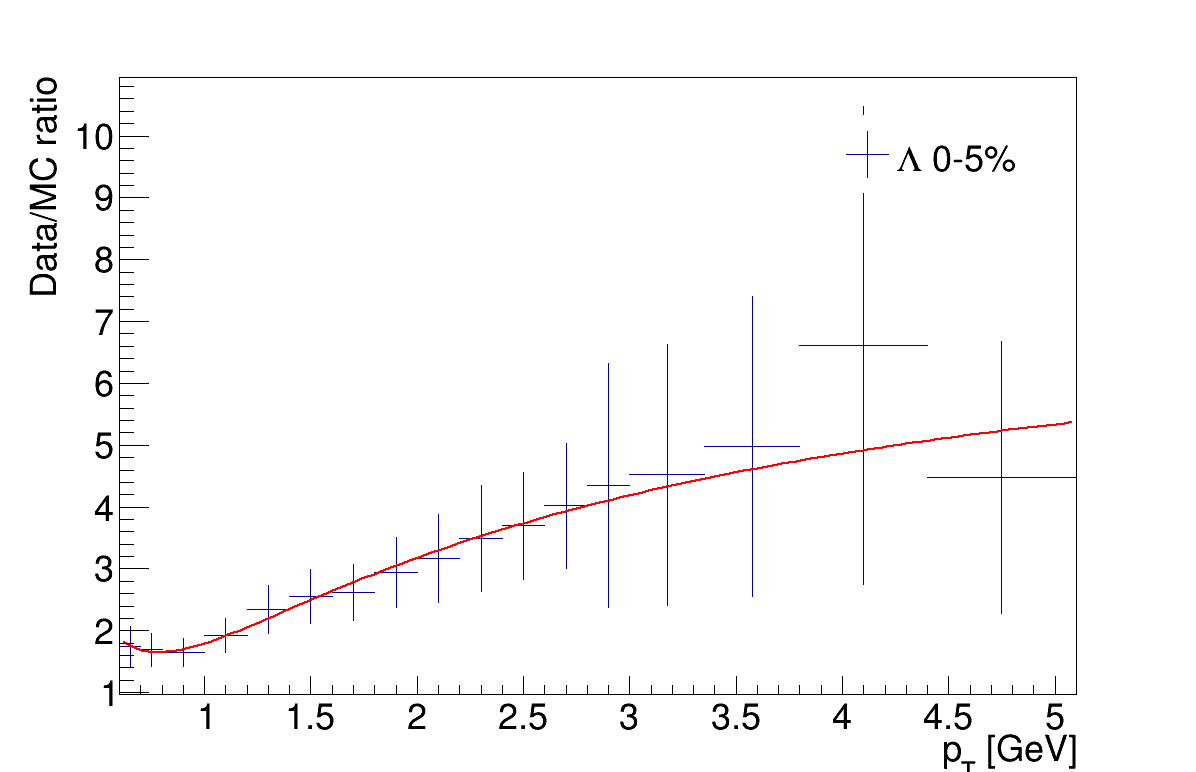
\includegraphics[width=0.24\linewidth]{detdeta/Figures/particle_reweighting_ratios/AMPT_lambda_0.png}
    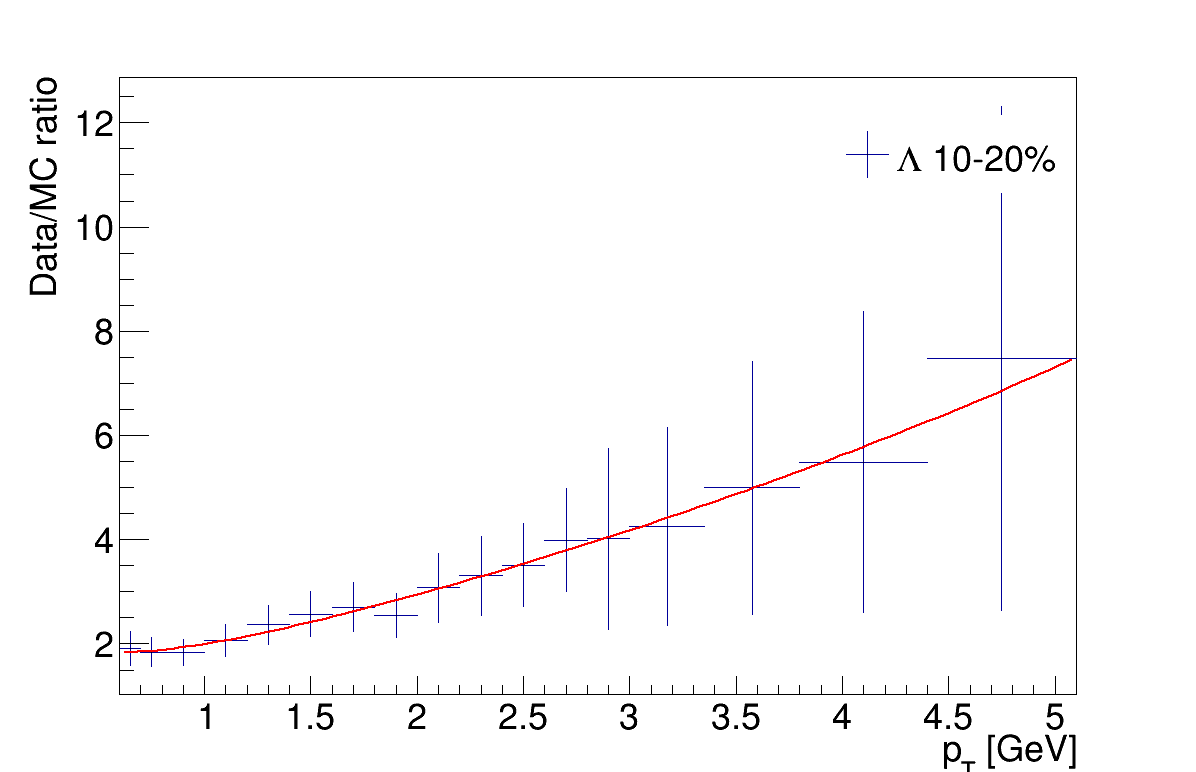
\includegraphics[width=0.24\linewidth]{detdeta/Figures/particle_reweighting_ratios/AMPT_lambda_1.png}
    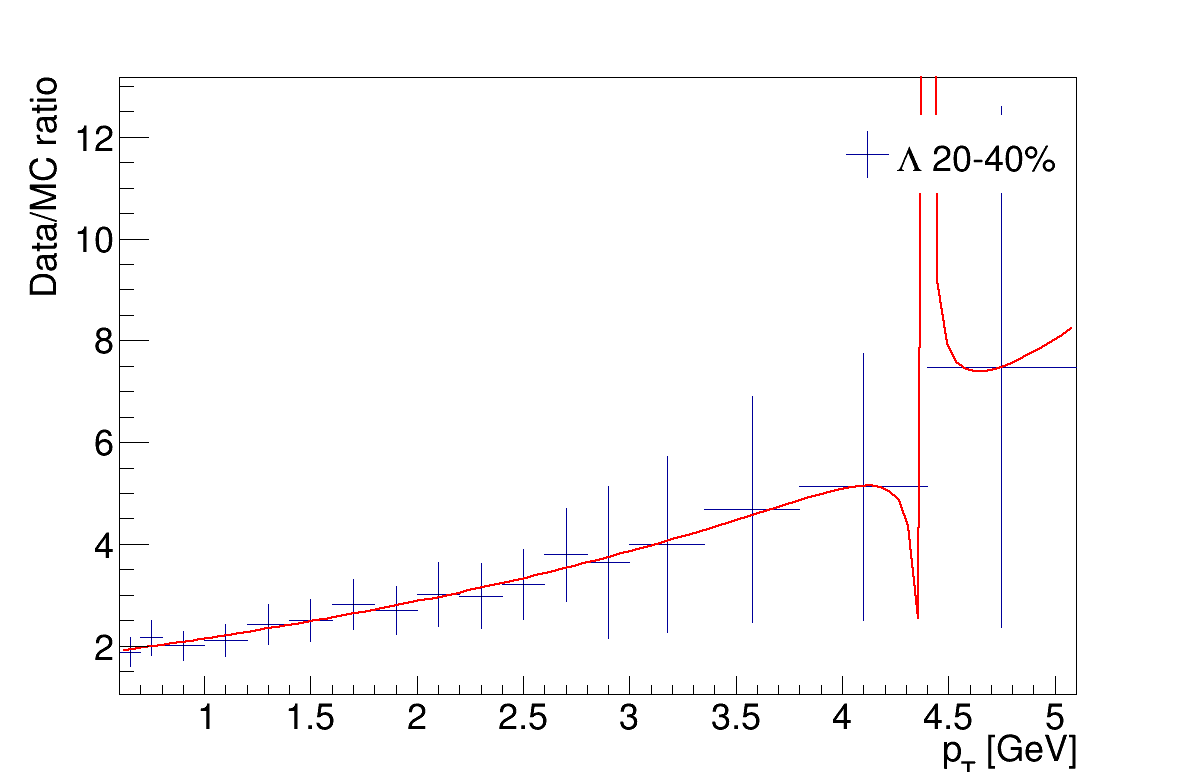
\includegraphics[width=0.24\linewidth]{detdeta/Figures/particle_reweighting_ratios/AMPT_lambda_2.png}
    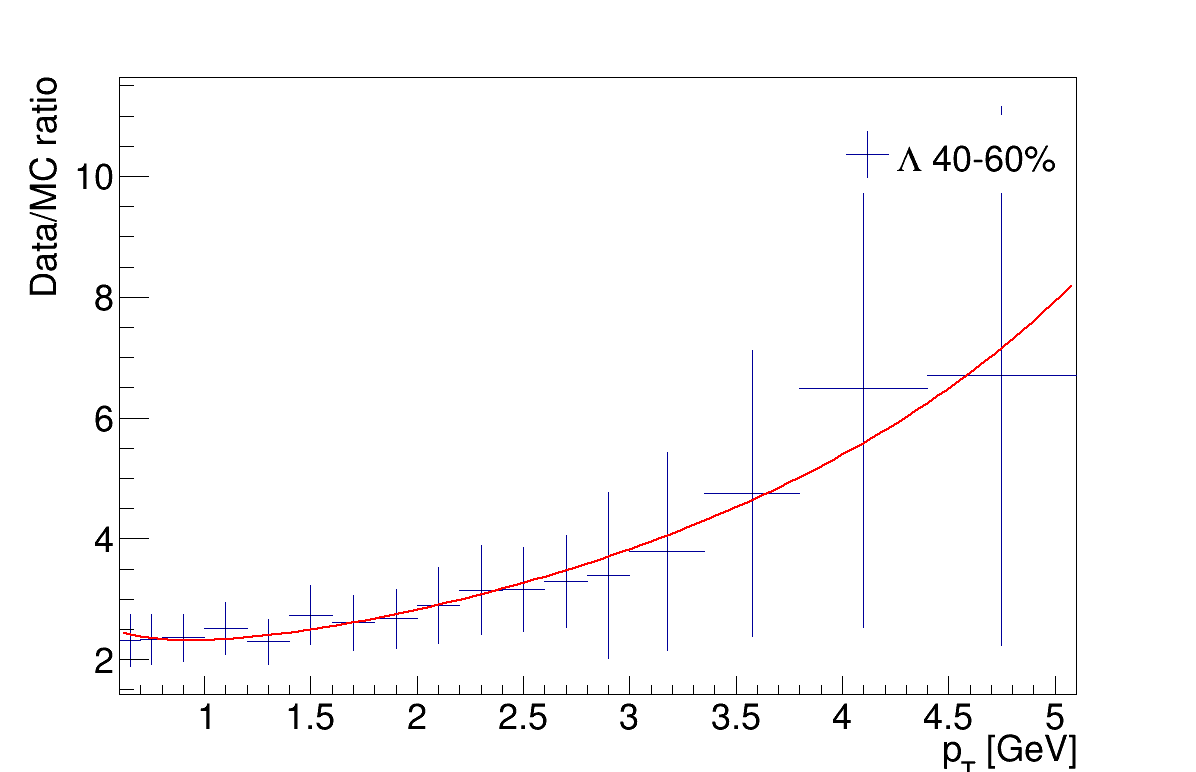
\includegraphics[width=0.24\linewidth]{detdeta/Figures/particle_reweighting_ratios/AMPT_lambda_3.png}
    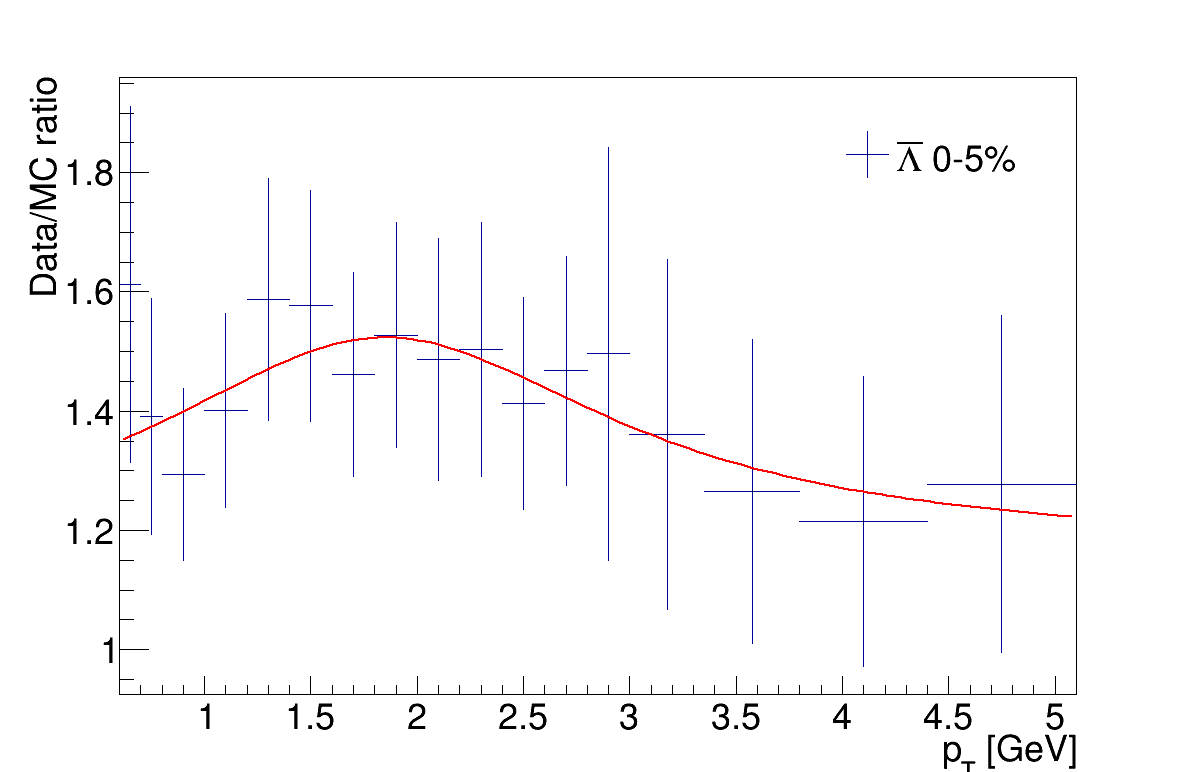
\includegraphics[width=0.24\linewidth]{detdeta/Figures/particle_reweighting_ratios/AMPT_lambda_bar_0.png}
    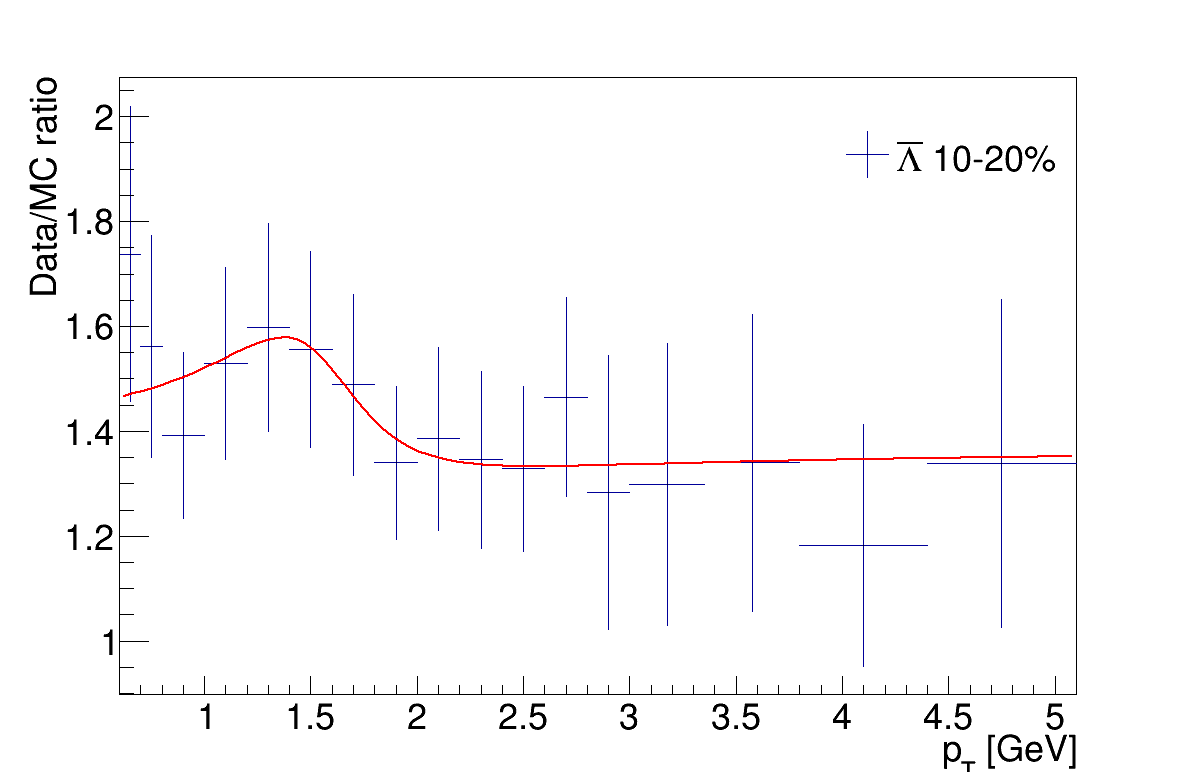
\includegraphics[width=0.24\linewidth]{detdeta/Figures/particle_reweighting_ratios/AMPT_lambda_bar_1.png}
    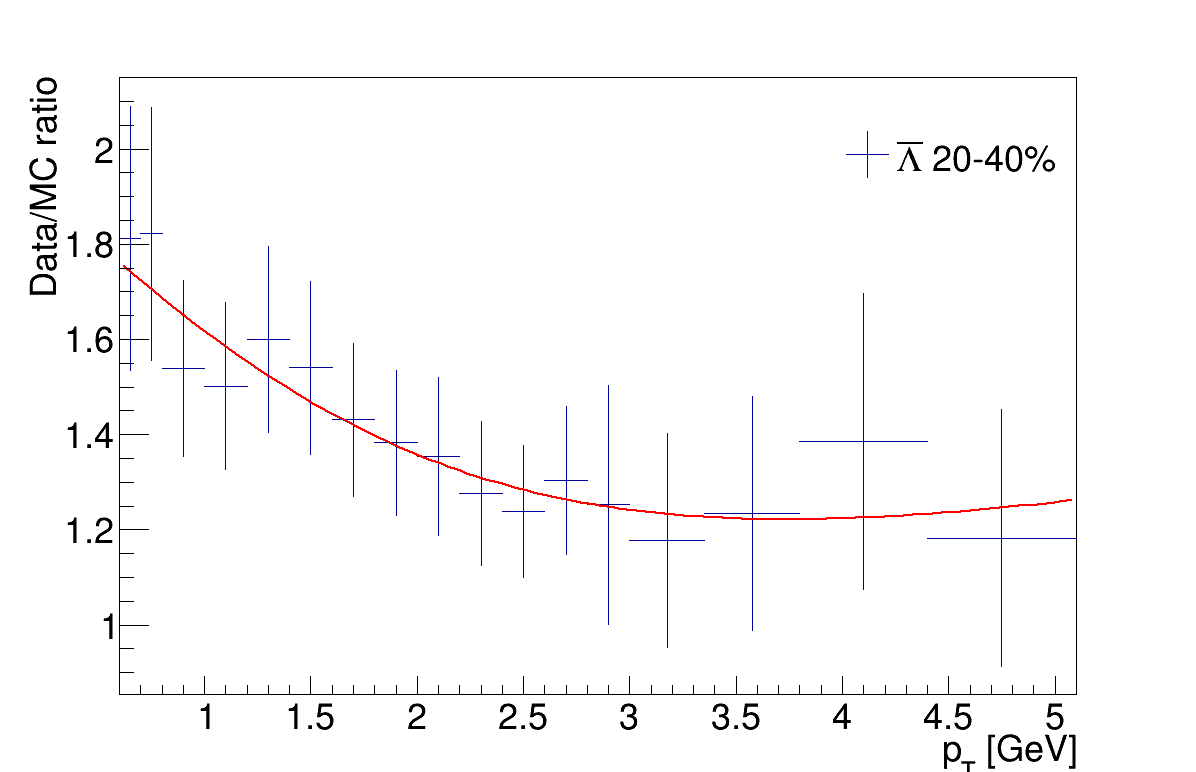
\includegraphics[width=0.24\linewidth]{detdeta/Figures/particle_reweighting_ratios/AMPT_lambda_bar_2.png}
    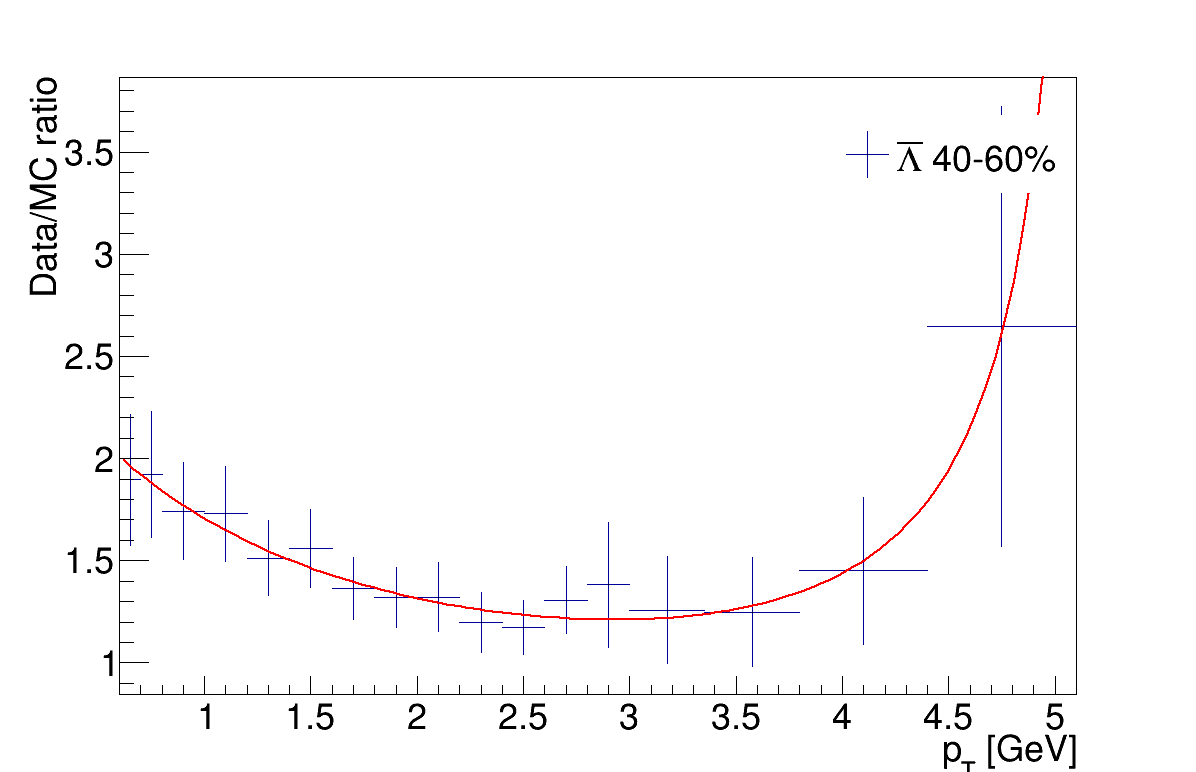
\includegraphics[width=0.24\linewidth]{detdeta/Figures/particle_reweighting_ratios/AMPT_lambda_bar_3.png}
    \caption{All data to MC ratios used in nominal AMPT reweighting method for protons, anti-protons, kaons, pions and lambda particles.}
    \label{fig:ampt_data_mc_particle_ratios}
\end{figure}

The effect of this particle reweighting methodology on the correction factors used to correct the detector-level \detdeta to truth-level \detdeta is shown in Fig.~\ref{fig:reweighted_corr_factors} for the EMCal, HCal and full calorimeter measurements. 
Fig.~\ref{fig:reweighted_corr_ratio} gives the ratio of the unweighted and reweighted correction factors.
\begin{figure}
    \centering
    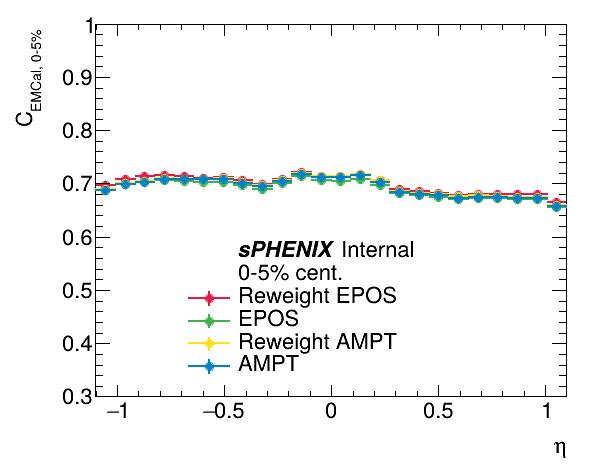
\includegraphics[width=0.24\linewidth]{detdeta/Figures/particle_reweighting_ratios/emcal_corr_0-5.png}
    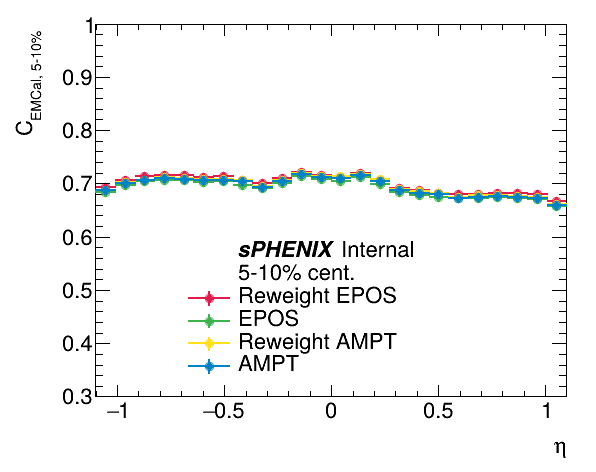
\includegraphics[width=0.24\linewidth]{detdeta/Figures/particle_reweighting_ratios/emcal_corr_5-10.png}
    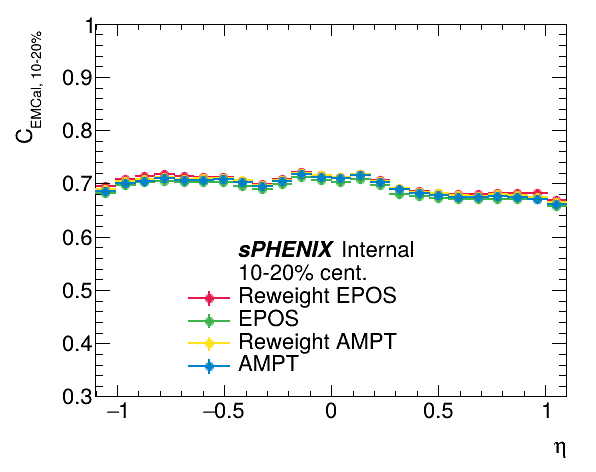
\includegraphics[width=0.24\linewidth]{detdeta/Figures/particle_reweighting_ratios/emcal_corr_10-20.png}
    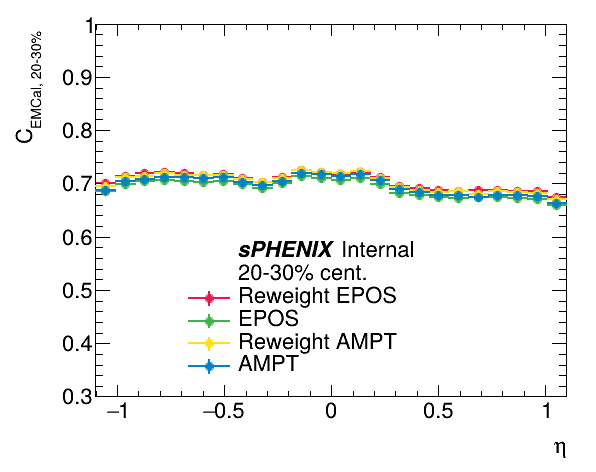
\includegraphics[width=0.24\linewidth]{detdeta/Figures/particle_reweighting_ratios/emcal_corr_20-30.png}
    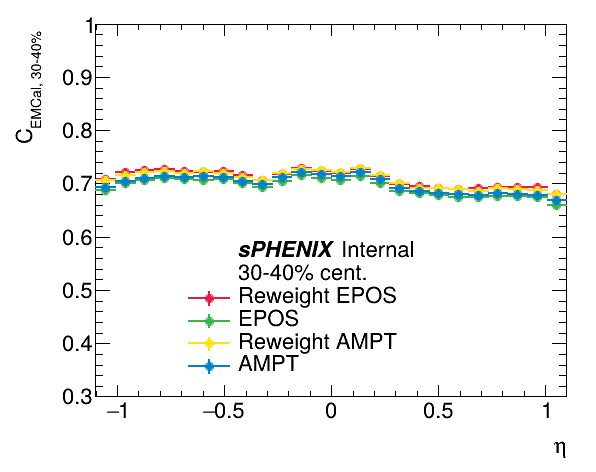
\includegraphics[width=0.24\linewidth]{detdeta/Figures/particle_reweighting_ratios/emcal_corr_30-40.png}
    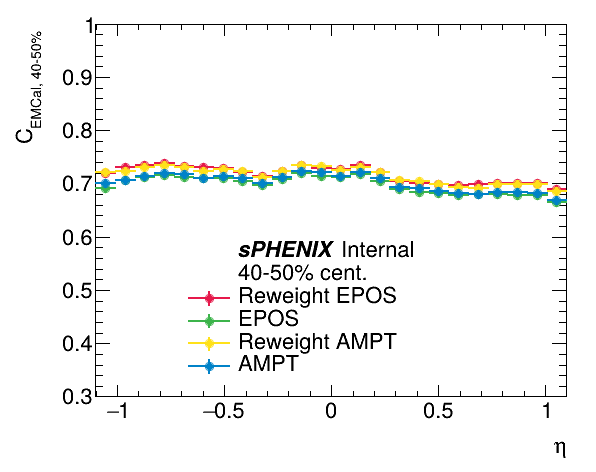
\includegraphics[width=0.24\linewidth]{detdeta/Figures/particle_reweighting_ratios/emcal_corr_40-50.png}
    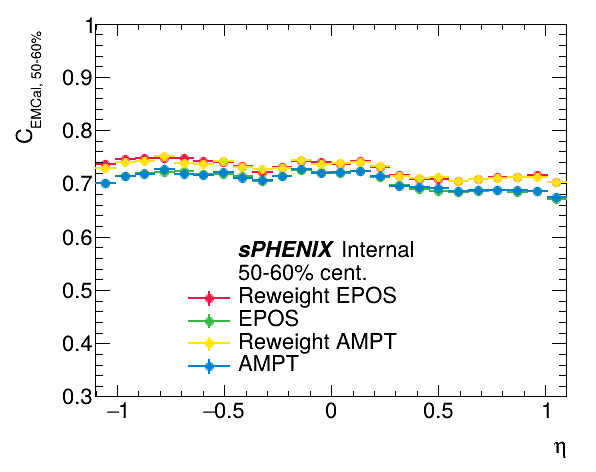
\includegraphics[width=0.24\linewidth]{detdeta/Figures/particle_reweighting_ratios/emcal_corr_50-60.png} \\
    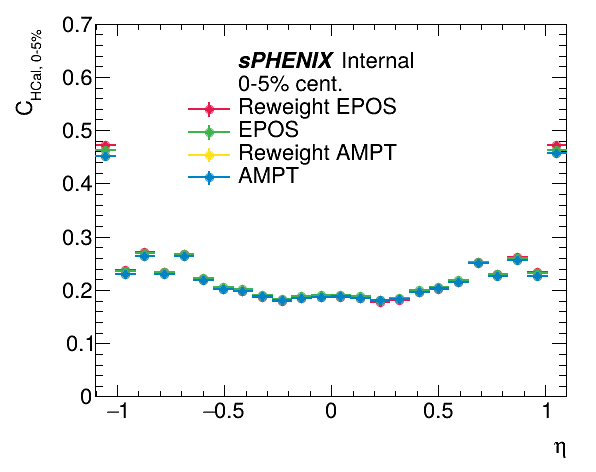
\includegraphics[width=0.24\linewidth]{detdeta/Figures/particle_reweighting_ratios/hcal_corr_0-5.png}
    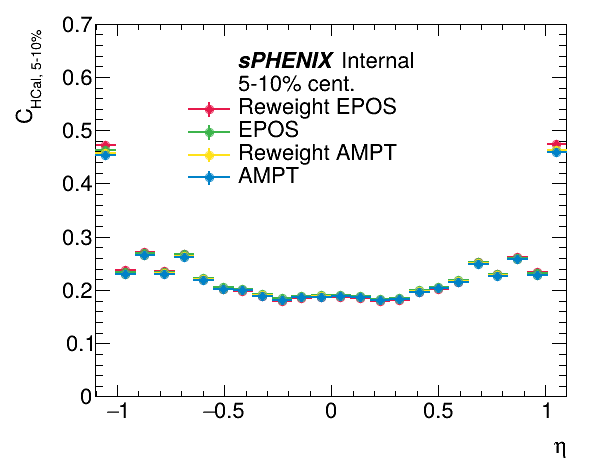
\includegraphics[width=0.24\linewidth]{detdeta/Figures/particle_reweighting_ratios/hcal_corr_5-10.png}
    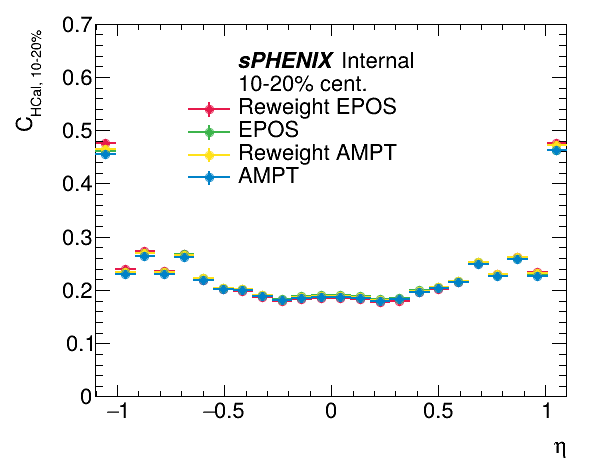
\includegraphics[width=0.24\linewidth]{detdeta/Figures/particle_reweighting_ratios/hcal_corr_10-20.png}
    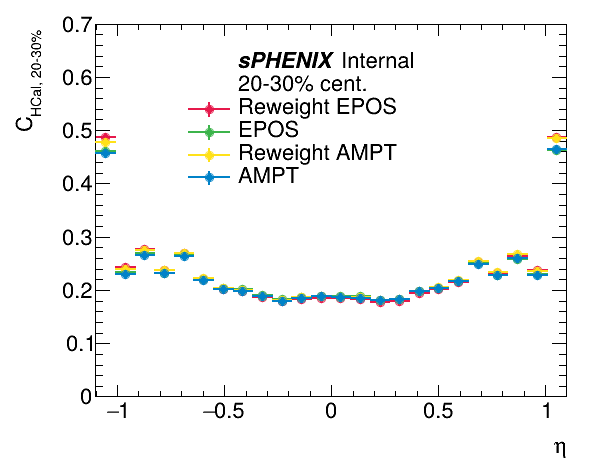
\includegraphics[width=0.24\linewidth]{detdeta/Figures/particle_reweighting_ratios/hcal_corr_20-30.png}
    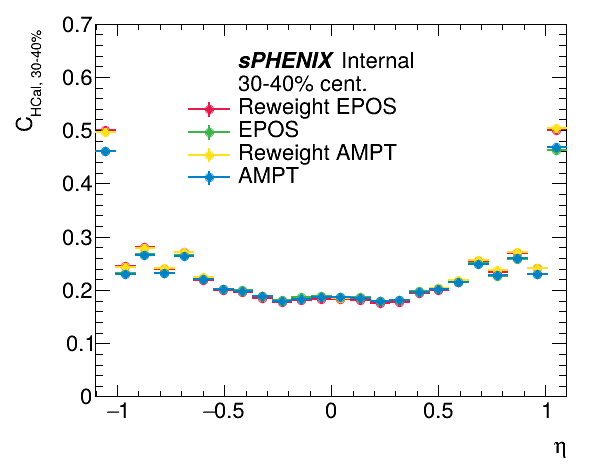
\includegraphics[width=0.24\linewidth]{detdeta/Figures/particle_reweighting_ratios/hcal_corr_30-40.png}
    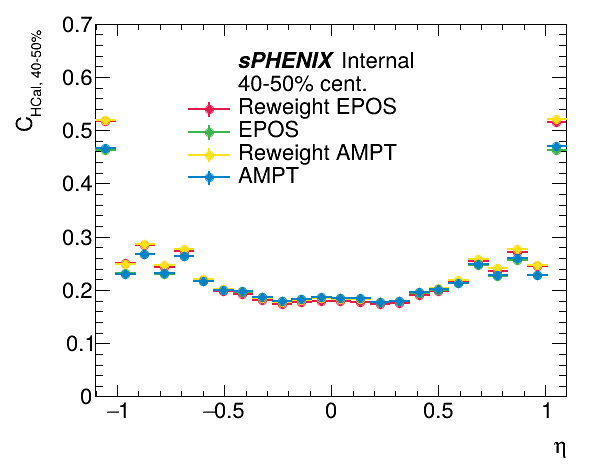
\includegraphics[width=0.24\linewidth]{detdeta/Figures/particle_reweighting_ratios/hcal_corr_40-50.png}
    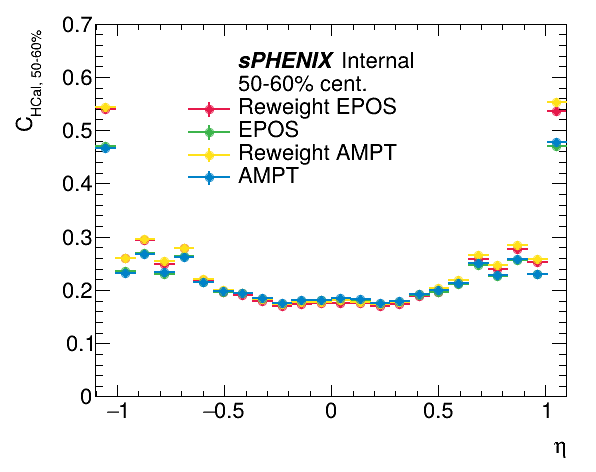
\includegraphics[width=0.24\linewidth]{detdeta/Figures/particle_reweighting_ratios/hcal_corr_50-60.png} \\
    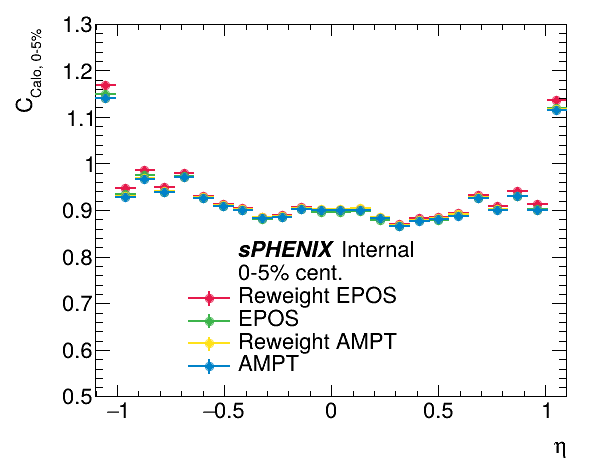
\includegraphics[width=0.24\linewidth]{detdeta/Figures/particle_reweighting_ratios/calo_corr_0-5.png}
    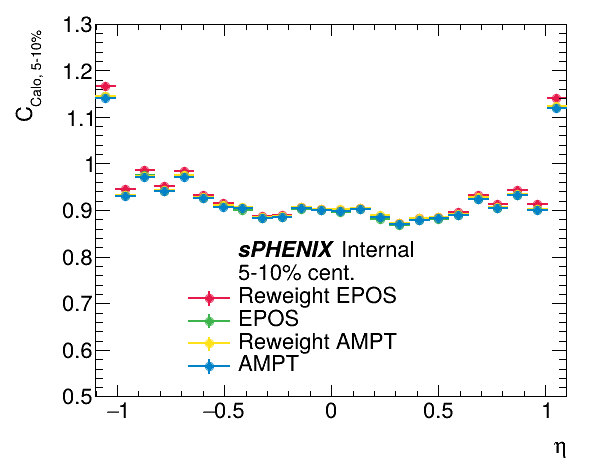
\includegraphics[width=0.24\linewidth]{detdeta/Figures/particle_reweighting_ratios/calo_corr_5-10.png}
    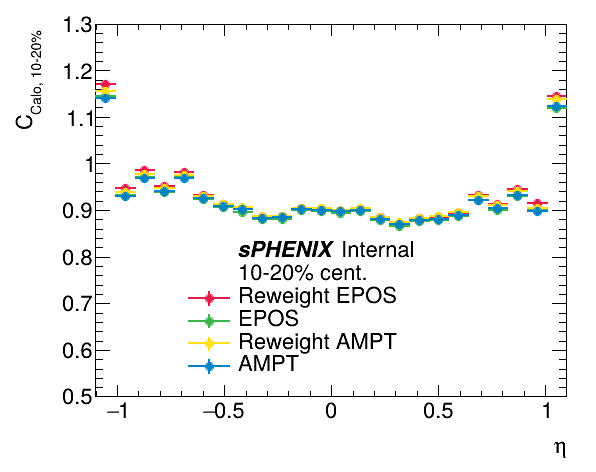
\includegraphics[width=0.24\linewidth]{detdeta/Figures/particle_reweighting_ratios/calo_corr_10-20.png}
    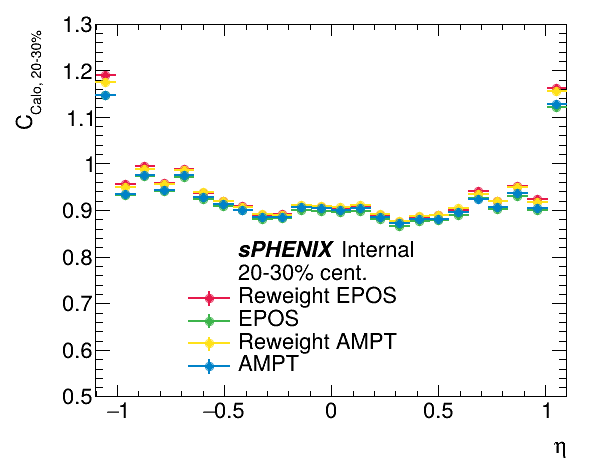
\includegraphics[width=0.24\linewidth]{detdeta/Figures/particle_reweighting_ratios/calo_corr_20-30.png}
    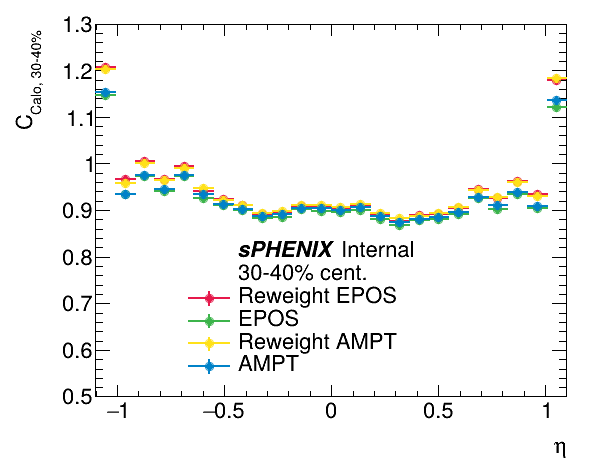
\includegraphics[width=0.24\linewidth]{detdeta/Figures/particle_reweighting_ratios/calo_corr_30-40.png}
    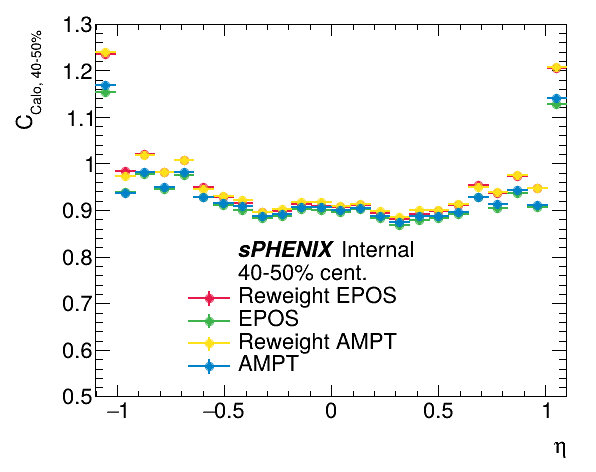
\includegraphics[width=0.24\linewidth]{detdeta/Figures/particle_reweighting_ratios/calo_corr_40-50.png}
    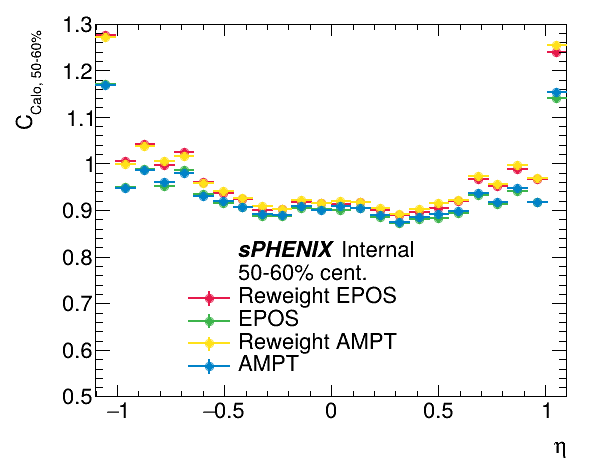
\includegraphics[width=0.24\linewidth]{detdeta/Figures/particle_reweighting_ratios/calo_corr_50-60.png}
    \caption{Effect of reweighting on the correction factors for the EMCal (top), HCal (middle) and full calorimeter for all centrality bins in the analysis.}
    \label{fig:reweighted_corr_factors}
\end{figure}

\begin{figure}
    \centering
    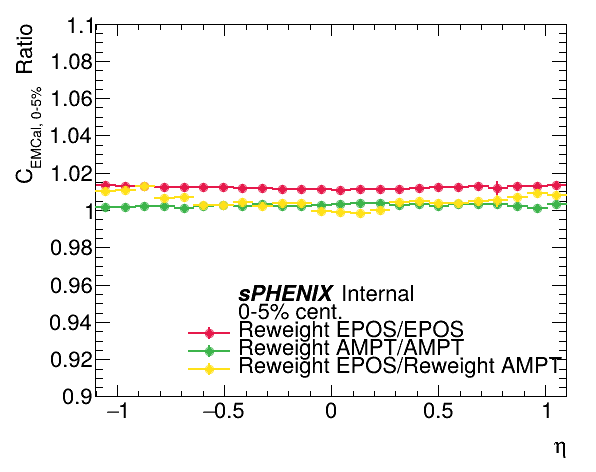
\includegraphics[width=0.24\linewidth]{detdeta/Figures/particle_reweighting_ratios/emcal_ratio_0-5.png}
    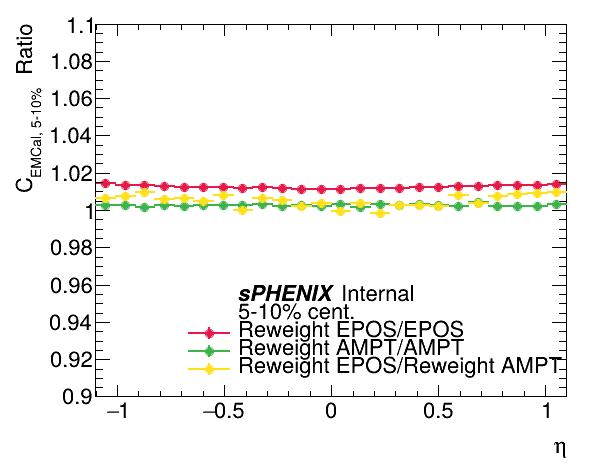
\includegraphics[width=0.24\linewidth]{detdeta/Figures/particle_reweighting_ratios/emcal_ratio_5-10.png}
    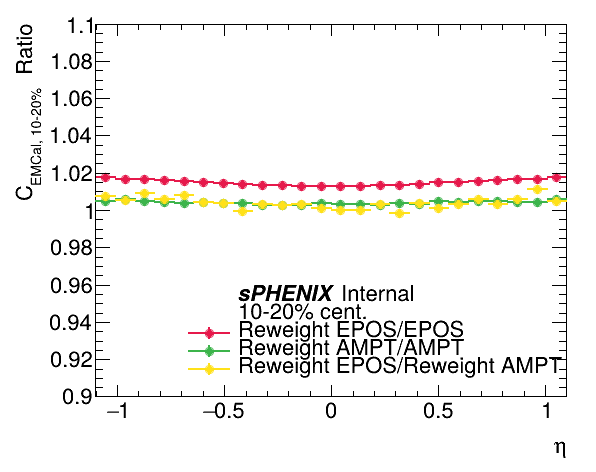
\includegraphics[width=0.24\linewidth]{detdeta/Figures/particle_reweighting_ratios/emcal_ratio_10-20.png}
    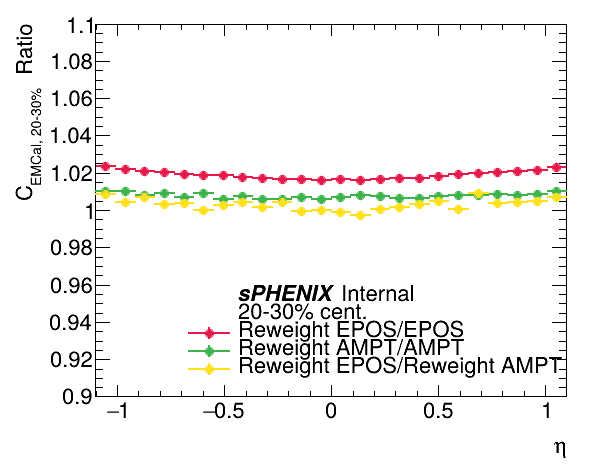
\includegraphics[width=0.24\linewidth]{detdeta/Figures/particle_reweighting_ratios/emcal_ratio_20-30.png}
    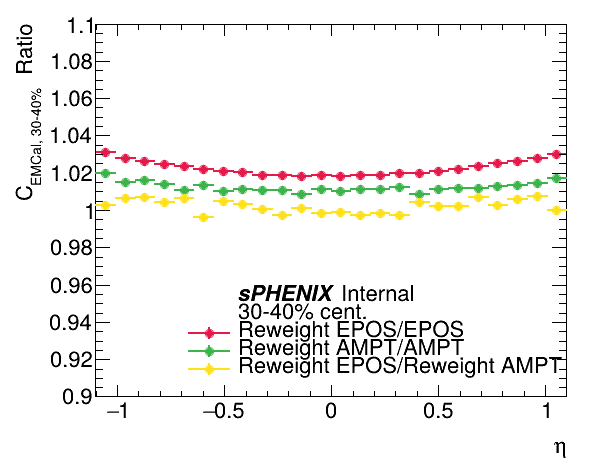
\includegraphics[width=0.24\linewidth]{detdeta/Figures/particle_reweighting_ratios/emcal_ratio_30-40.png}
    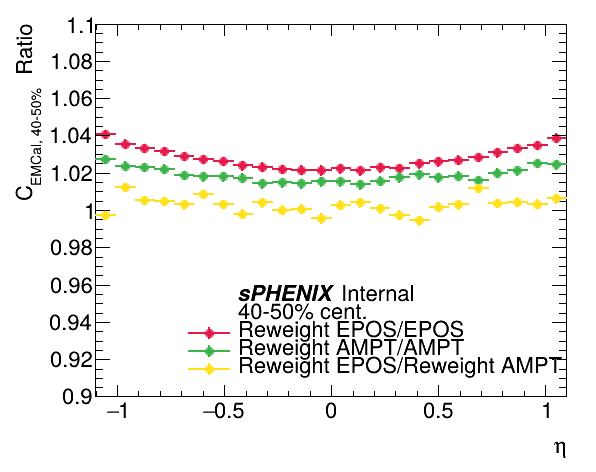
\includegraphics[width=0.24\linewidth]{detdeta/Figures/particle_reweighting_ratios/emcal_ratio_40-50.png}
    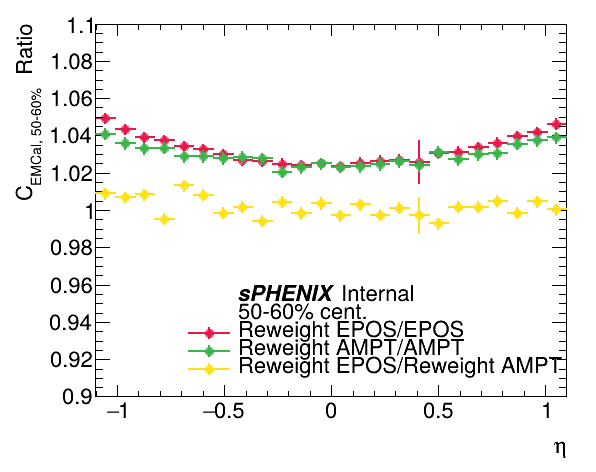
\includegraphics[width=0.24\linewidth]{detdeta/Figures/particle_reweighting_ratios/emcal_ratio_50-60.png} \\
    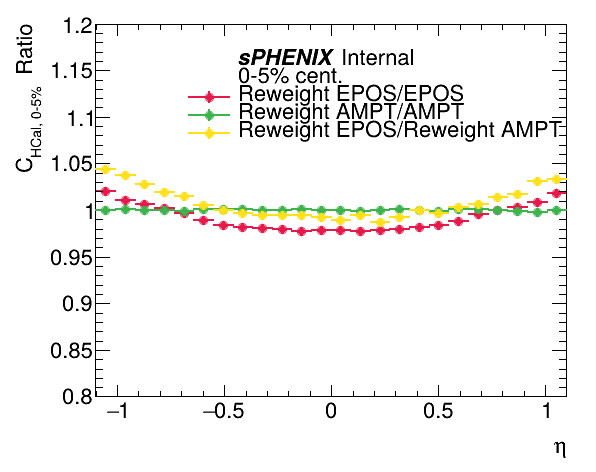
\includegraphics[width=0.24\linewidth]{detdeta/Figures/particle_reweighting_ratios/hcal_ratio_0-5.png}
    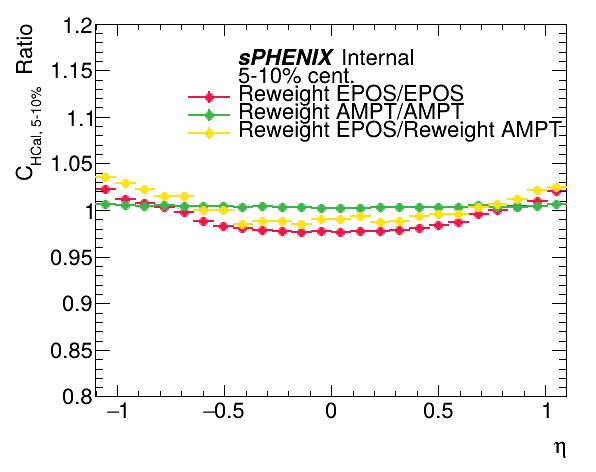
\includegraphics[width=0.24\linewidth]{detdeta/Figures/particle_reweighting_ratios/hcal_ratio_5-10.png}
    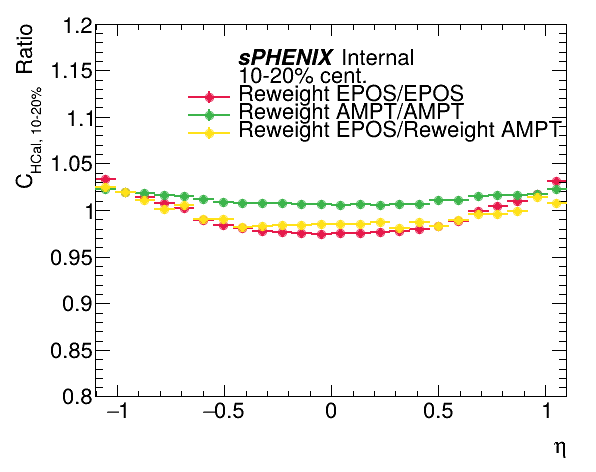
\includegraphics[width=0.24\linewidth]{detdeta/Figures/particle_reweighting_ratios/hcal_ratio_10-20.png}
    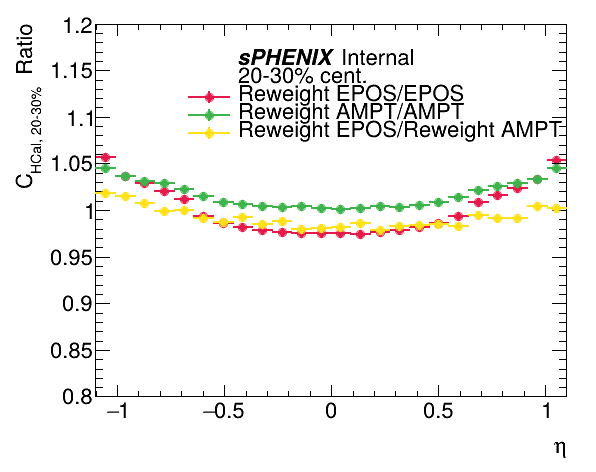
\includegraphics[width=0.24\linewidth]{detdeta/Figures/particle_reweighting_ratios/hcal_ratio_20-30.png}
    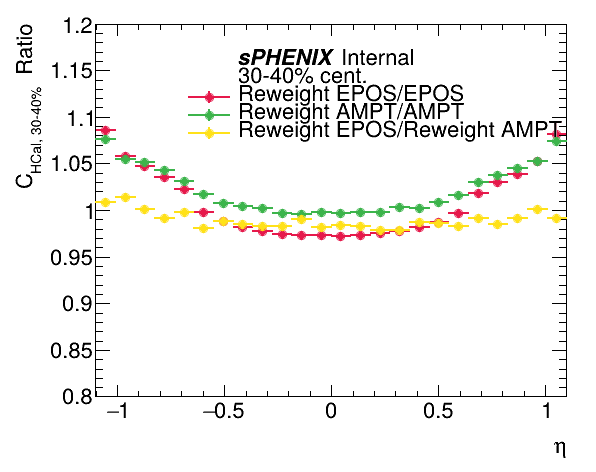
\includegraphics[width=0.24\linewidth]{detdeta/Figures/particle_reweighting_ratios/hcal_ratio_30-40.png}
    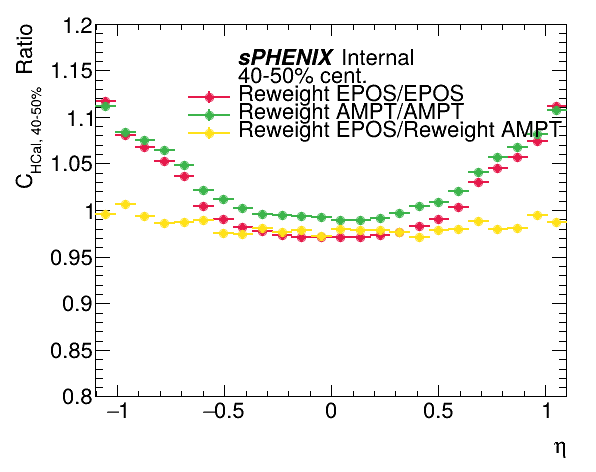
\includegraphics[width=0.24\linewidth]{detdeta/Figures/particle_reweighting_ratios/hcal_ratio_40-50.png}
    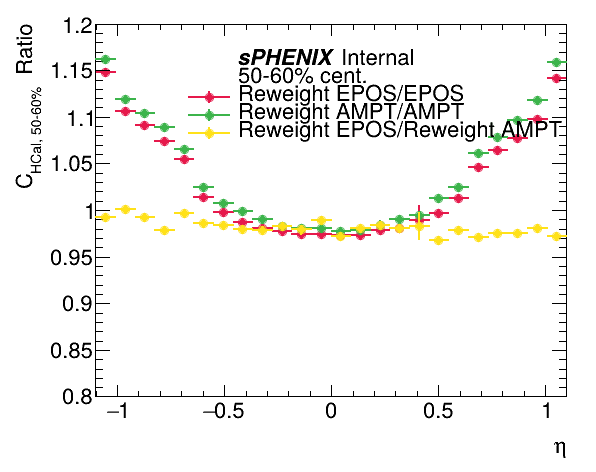
\includegraphics[width=0.24\linewidth]{detdeta/Figures/particle_reweighting_ratios/hcal_ratio_50-60.png} \\
    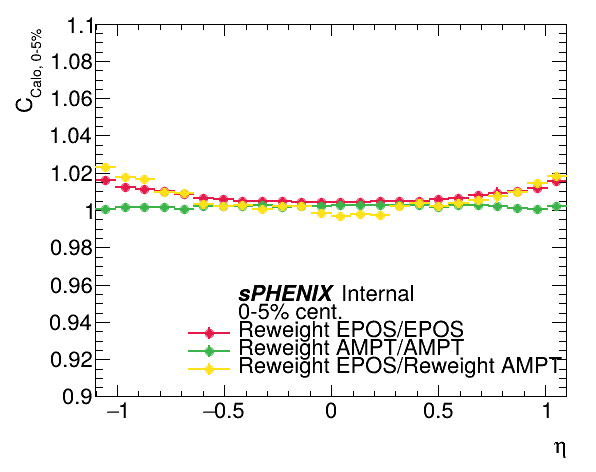
\includegraphics[width=0.24\linewidth]{detdeta/Figures/particle_reweighting_ratios/calo_ratio_0-5.png}
    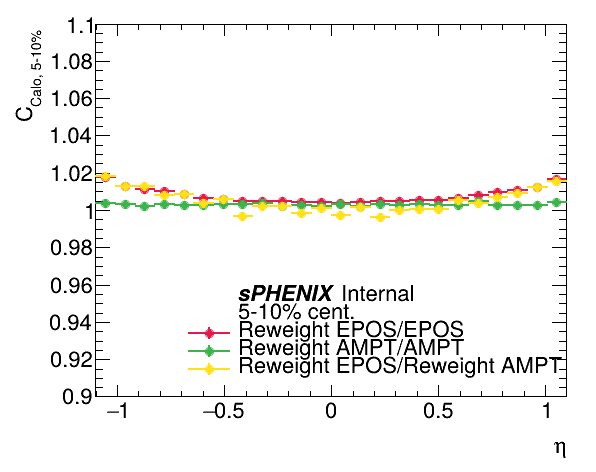
\includegraphics[width=0.24\linewidth]{detdeta/Figures/particle_reweighting_ratios/calo_ratio_5-10.png}
    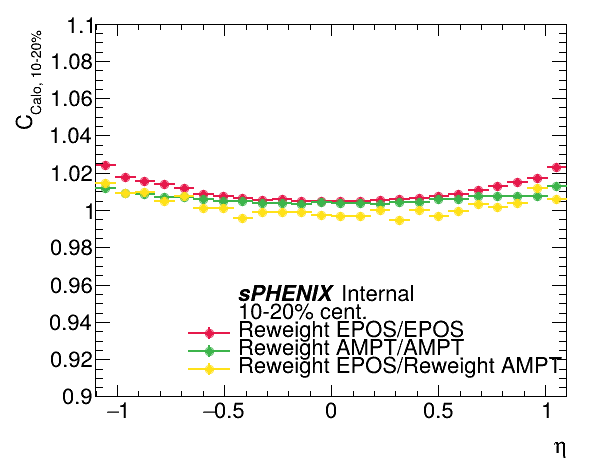
\includegraphics[width=0.24\linewidth]{detdeta/Figures/particle_reweighting_ratios/calo_ratio_10-20.png}
    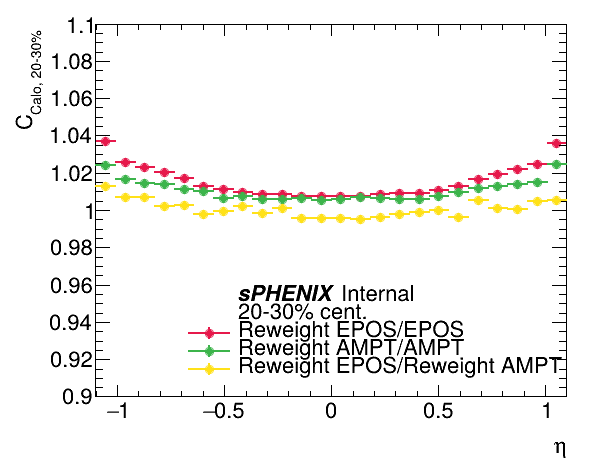
\includegraphics[width=0.24\linewidth]{detdeta/Figures/particle_reweighting_ratios/calo_ratio_20-30.png}
    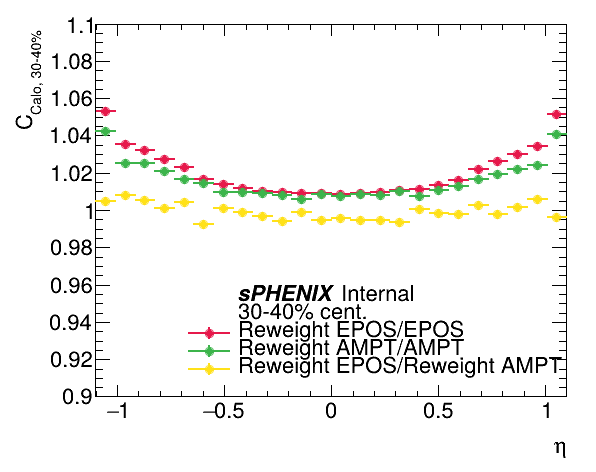
\includegraphics[width=0.24\linewidth]{detdeta/Figures/particle_reweighting_ratios/calo_ratio_30-40.png}
    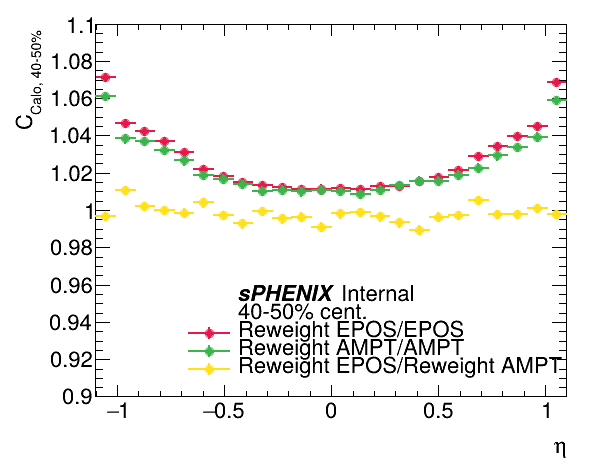
\includegraphics[width=0.24\linewidth]{detdeta/Figures/particle_reweighting_ratios/calo_ratio_40-50.png}
    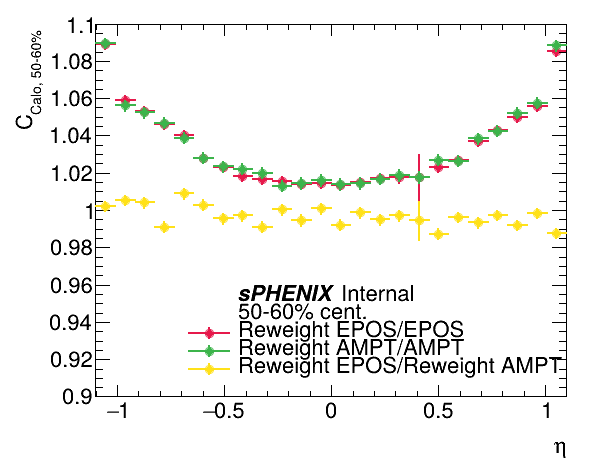
\includegraphics[width=0.24\linewidth]{detdeta/Figures/particle_reweighting_ratios/calo_ratio_50-60.png}
    \caption{Ratio of correction factors with and without the particle reweighting applied for the EMCal (top) and HCal (bottom) for all centrality bins in the analysis.}
    \label{fig:reweighted_corr_ratio}
\end{figure} 